% kate: encoding iso-8859-1
% changed to utf8 by Karol Kozioł
\RequirePackage{fix-cm} % Improves appearance of some cm-super fonts
\RequirePackage[l2tabu, orthodox]{nag}    % warns about some obsolete latex constructs
\documentclass[
   12pt,                % font size 12pt
   a4paper,             % layout for DIN A4
   oneside,             % layout for one sided printing
   headinclude,         % include head in layout computation
   headsepline,         % horizontal line below head
   BCOR12mm,            % correction for fixation
   DIV16,               % DIV-value for creating the print space, (see scrguien.pdf)
   halfparskip,         % spacing between paragraphs
   openany,             % chapters may start on even and odd pages
   bibtotoc,            % put bibliography into table of contents
   pointlessnumbers,    % chapter numbers without full stop
   tablecaptionabove,   % use table headings with correct spacing
   fleqn                % float equations to left margin
]{scrbook}[2007/12/24]  % scrbook-Version min. v2.98 from 2007/12/24

%\usepackage[latin1]{inputenc}    % change to your encoding (e.g. utf8)
\usepackage[utf8]{inputenc}
\usepackage[T1]{fontenc}         % correct pdf output (correct umlaut charaters)
%\usepackage{lmodern}             % fonts for pdf-file creation (use Type1 instead of Type3) - only needed, if cmsuper is not installed
%                                 % check the resulting pdf-file: fonts should been embedded, subsetted and of type 1 (NOT type 3!)
\usepackage[intlimits]{amsmath}  % place the subscripts and superscripts in the right position
\usepackage{amsfonts}            % additional fonts like \mathbb, \mathfrak
\usepackage{amssymb}             % additional symbols
\usepackage{url}                 % support for urls
\usepackage{natbib}
\usepackage{longtable}  % For multipage tables!

% \usepackage{apalike}            % bibliography package
% \usepackage{ngerman}             % new german orthography
\usepackage{scrpage2}            % head and foot layout
\usepackage{ushort}              % complex values require an underline (use \ushort or \ushortw)
\usepackage{units}               % package for setting units in a typographically correct way (e.g. \unit[3]{cm})
\usepackage{booktabs}            % package provides additional commands to enhance the quality of tables
\usepackage{datetime}            % provides \pdfdate command

\numberwithin{equation}{section} % amsmath: numbering equations
\bibliographystyle{authordate1}       % use a DIN style for the bibliography
\pagestyle{scrheadings}          % enable scrheadings layout for head and foot

\ifx\pdfoutput\undefined
 % non pdflatex settings (normal latex compiler assumed)
 \usepackage[dvips]{graphicx}
\else
 % different settings for the pdflatex compiler
 \usepackage[pdftex]{graphicx}
 \usepackage{epstopdf}           % enables automatic conversion from .eps to .pdf graphic files; run MikTeX as "latex --enable-write18"
 \usepackage[pdftex,plainpages=false]{hyperref}

 \usepackage{lineno}

 \pdfcompresslevel=9
 \pdfinfo{
    /CreationDate (D:20160501110000) % date format is year(4) month(2) day(2) hour(2) minute(2) second(2)
    /ModDate      (D:\pdfdate)
 }
 \hypersetup{
    pdftitle    = {thesis title},
    pdfsubject  = {thesis subject},
    pdfauthor   = {your name},
    pdfkeywords = {},
    colorlinks  = {true},
    linkcolor   = {black},
    citecolor   = {black},
    urlcolor    = {black}
 }
\fi


\renewcommand{\bibname}{Bibliography}   % new name for the bibiography
\renewcommand{\figurename}{Figure}           % new name for the figure
\renewcommand{\listfigurename}{List of Figures} % new name for the list of figures


\makeindex

\begin{document}
\newcommand{\dissnum}{XXXXX}
\renewcommand{\title}{Screening Meter Data: \\Characterization of Temporal Energy Data from Large Groups of Non-Residential Buildings}
\newcommand{\degree}{DOCTOR OF SCIENCES of ETH ZURICH}
\newcommand{\shortdegree}{(Dr. sc. ETH Zurich)}
\renewcommand{\author}{Clayton C. Miller}
\newcommand{\acatitle}{Masters of Science (MSc.) Building, National University of Singapore\\
Masters of Architectural Engineering (MAE), Univ. of Nebraska}
\newcommand{\dateofbirth}{22 January 1984}
\newcommand{\citizen}{the United States of America}
\newcommand{\examiner}{Prof. Dr. Arno Schlueter}
\newcommand{\coexaminera}{Prof. Dr. Stefan Mueller Arisona}
% \newcommand{\coexaminerc}{Prof. Dr. X}
% \newcommand{\coexaminera}{Prof. Dr. X}

% \maketitle
\frontmatter
\begin{titlepage}
    \setlength{\baselineskip}{8mm}
    \begin{center}
    	{\large\noindent Diss.\ ETH No.\ \dissnum}
    \end{center}
    \vfill
    \begin{center}
        \bfseries\sffamily\Huge\title %\\[5mm]
%        \LARGE\subtitle
    \end{center}
    \vfill
    \begin{center}
        \large A thesis submitted to attain the degree of \\[1mm]
        {\bfseries\sffamily\degree} \\[1mm]
        \shortdegree
    \end{center}
    \vspace{0.5\fill}
    \begin{center}
        \large presented by \\[1mm]
         {\bfseries\sffamily\uppercase\expandafter{\author}} \\[1mm]
         \acatitle \\
         born on \dateofbirth \\
         citizen of \citizen
    \end{center}
    \vspace{0.5\fill}
    \begin{center}
         \large accepted on the recommendation of \\
         \examiner, examiner \\
         \coexaminera, co-examiner \\
         % \coexaminerb, co-examiner \\
         % \coexaminerc, co-examiner
    \end{center}
    \vspace{0.5\fill}
    \begin{center}
         \large\number\year
    \end{center}
    \cleardoublepage	
\end{titlepage}

\chapter{Abstract}

This study focuses on the screening of characteristic data from the ever-expanding sources of raw, temporal sensor data from commercial buildings. A two-step framework is presented that extracts statistical, model-based, and pattern-based behavior from two real-world data sets. The first collection is from 507 commercial buildings extracted from various case studies and online data sources from around the world. The second collection is advanced metering infrastructure (AMI) data from 1,600 buildings. The goal of the framework is to reduce the expert intervention needed to utilize measured raw data in order to extract information such as building use type, performance class, and operational behavior. The first step is feature extraction and it utilizes a library of temporal data mining techniques to filter various phenomenon from the raw data. This step transforms quantitative raw data into qualitative categories that are presented in heat map visualizations for interpretation. In the second step, or the investigation, a supervised learning technique is tested in the ability to assign impact scores to the most important features from the first step. The efficacy of estimating variable causality of the characterized performance is tested to determine scalability amongst a heterogeneous sample of buildings. In the first set of case studies, characterization as compared to a baseline was three times more accurate in characterizing primary buildng use type, almost twice for performance class, and over four times for building operations type. For the AMI data, characterizing the standard industry class was improved by 27\% and predicting the success of energy savings measures was improved by 18\%. Qualitative insight from several campus case study interviews are discussed as well. The usefulness of the approaches was discussed in the context of campus building operations.
\chapter{Kurzfassung}

Diese Studie behandelt das Sichten, Sortieren und Bearbeiten charakteristischer Zeitreihen aus stark wachsenden Quellen fu\"r rohe Sensordaten in kommerziellen Gebäuden. Ein zweistufiges Vorgehen wird präsentiert, das statistische, modellbasierte und Muster-basierte Verhaltensweisen von zwei Datensätzen extrahiert. Der erste Datensatz beinhaltet Daten von 507 kommerziellen Gebäuden, zusammengetragen aus verschiedenen Fallbeispielen und online Datenquellen aus der ganzen Welt. Der zweite Datensatz beinhaltet Daten von Advanced Metering Infrastructure (AMI) von 1,600 Gebäuden. Das Ziel der vorgestellten Methode ist das Reduzieren benötigter Experteneingriffe, um gemessene Rohdaten benutzen zu können zum Erhalten von Information wie Gebäudenutzungstyp, Performance Klasse und Betriebsverhalten. Im ersten Schritt, dem Extrahieren von Charakteristiken, werden durch das Benutzen einer Bibliothek von Data Mining Techniken verschiedene Phänomene aus den Rohdaten herausgefiltert. Dieser Schritt transformiert quantitative Rohdaten zu qualitativen Kategorien, die durch Heat Map Visualisierungen präsentiert und interpretiert werden. Im zweiten Schritt, der Datenuntersuchung, wird eine Supervised Learning Technique auf die Möglichkeit hin getestet, den wichtigsten Charakteristiken aus dem ersten Schritt eine Auswertung der Auswirkungen zuzuordnen. Um das Hochskalieren für heterogene Gebäudeparks zu untersuchen wird die Wirksamkeit getestet, variable Kausalzusammenhänge der charakterisierten Performance zu schätzen. In den Fallstudien im ersten Datensatz war die Bestimmung des primären Gebäudenutzungstyps dreimal treffender, die Bestimmung der Performance Klasse fast zweimal treffender und die Bestimmung des Betriebsverhaltenstyps über viermal treffender als für ein Basisvorgehen. Für die AMI Daten wurde die Charakterisierung der Standard Industrie Klasse  um 27\% verbessert, die Prognose der Erfolgsrate von Energiesparmassnahmen um 18\% verbessert. Interviews mit Akteuren von mehreren Schulanlagen werden diskutiert bezüglich ihrer qualitativen Einblicke und bezüglich der Nützlichkeit der vorgestellten Ansätze im Kontext des Betriebs von Schulanlagen. 

\chapter{Acknowledgements}

This work is the result of years of rumination about buildings and what might make the biggest impact in understanding the way they are operated. This end goal is important, but it is not as meaningful as the process and the people who provided support, insight and love to help achieve it. 

The Architecture and Building Systems Group in Zurich provided me with an environment and camaraderie to make this work possible. Prof. Arno Schlueter was an outstanding leader who organized the smartest group of people I've ever worked with. Daren needs to be thanked for cheese, hugs, jokes, and runs through the woods. Valerie was always there to answer questions and help navigate all the administrative challenges. PJ, Bratislav, Geroid, Anya, Christian, and Michele provided guidance and stimulating conversations. The Singapore FCL, 3for2 and UWC teams, including Adam, Yuzhen, Marcel, Forrest, Simon and Kenny and others made it possible and enjoyable to complete this work in Singapore. 

I'd like to thank all the external collaborators who made the data collection and analysis process possible. The facilities management teams from the various case study campuses provided the data, insight, and effort that made this work possible. Greg Fanslow and the VEIC team were invaluable in the analysis of AMI data.

My friends in Singapore, Zurich and the USA are too numerous to specifically mention, but their friendship is what made the process possible through both the good and difficult times. 

My family is the foundation for my work. Mel and Jerry provided unwavering support and love, despite my insistence to live my dreams abroad. Rick, Cassie, Kim, and Jarred were all there as supports and huge role models for myself and their beautiful families. Ethan, Leah, Derick, Aaron, Issac, Lily, Autumn, and Emily are my inspiration. 



\tableofcontents
%\listoftables
\listoffigures

\linespread{1.2}\selectfont                    % switch to 1.5 linespacing
\linenumbers

\mainmatter
\chapter{Introduction}
\label{sec:intro}
The built and urban environments have a significant impact on resource consumption and greenhouse gas emissions in the world. The United States is the world's second largest energy consumer, and buildings there account for 41\% of energy consumed\footnote{As of 2014, according to: \url{http://www.eia.gov/}}. The most extensive meta-analysis thus far of non-residential existing buildings showed a median opportunity of 16\% energy savings potential by using cost-effective measures to remedy performance deficiencies \citep{mills_building_2011}. Simply stated, roughly 6\% of the energy consumed in the U.S. could be easily mitigated - a figure that would eventually grow to an annual energy savings potential of \$30 billion and 340 megatons of C02 by the year 2030. Beyond saving energy, money and mitigating carbon, the impact of building performance improvement also extends to the health, comfort and satisfaction of the people who use buildings.

It is mysterious that these performance improvements are not rapidly being identified and implemented on a massive scale across the world’s building stock given the incentives and amount of research focused on building optimization in the fields of Architecture, Engineering and Computer Science. A comprehensive study of building performance analysis was completed by the California Commissioning Collaborative (CACx) to characterize the technology, market, and research landscape in the United States. Three of the key tasks in this project focused on establishing the state of the art \citep{effinger_building_2010}, characterizing available tools and the barriers to adoption \citep{ulickey_building_2010}, and establishing standard performance metrics \citep{greensfelder_building_2010}. These reports were accomplished through investigation of the available tools and technologies on the market as well as discussions and surveys with building operators and engineers. The common theme amongst the interviews and case studies was the \emph{lack of time and expertise} on the part of the dedicated operations professionals. The findings showed that installation time and cost was driven by the need for an engineer to develop a full understanding of the building and systems. These barriers reduce the implementation of performance improvements.

% These results are interpreted as a potential need for techniques that take into consideration the people, process, and philosophy aspects of the performance analysis equation \citep{miller_applicability_2013}. 


In another study, Ruparathna et al. created a contemporary review of building performance analysis techniques for commercial and institutional buildings \citep{ruparathna_improving_2016}. This review was comprehensive in capturing approaches related to technical, organizational, and behavioral changes. The majority of publications considered fall within the domains of automated fault detection and diagnostics, retrofit analysis, building benchmarking, and energy auditing. These traditional techniques focus on one building or a small, related collection of buildings, such as a campus. Many require complex characteristic data about each building, such as it geometric dimensions, building materials, the age and type of mechanical systems, and other metadata, to execute the process. Once again, such detailed techniques rely on metadata that often doesn't exist in the field, thus contributing to the barriers listed above.

Another issue facing the building industry is the characterization of the commercial building stock for benchmarking, intervention targeting, and general understanding of the way modern buildings are being utilized and operated. The Commercial Building Energy Consumption Survey (CBECS) is the primary means of collecting a characteristic data about the global commercial building stock in the United States. This survey is conducted every four years, the latest in 2012 in which information on over 6,700 building around the U.S. was collected for characterization. A large amount of meta-data was collected about each building from categories such as size, vintage, geographic region, and principal activity. This data collection was done through the efforts about 250 interviewers across the country under the supervision of 17 field supervisors, three regional field managers, and a field director. This manpower was utilized over the course of over three years to characterize and document the commercial building stock.

% Studies have revealed that a lack of skilled professionals, time, and budget heavily contribute to this reality \citep{ulickey_building_2010,effinger_building_2010}. 

From these studies, it becomes apparent that the biggest barrier to achieving performance improvement in buildings is scalability. Architecture is a discipline founded with aesthetic creativity as a core tenet. Frank Lloyd Wright once stated, ``The mother art is architecture. Without an architecture of our own, we have no soul of our civilization.'' Designers rightfully strive for artistic and meaningful creations; this phenomenon results in buildings with not only distinctive aesthetics but also unique energy systems design, installation practices and different levels of organization within the data-creating components. In this dissertation, I show that an emerging mass of data from the built environment can facilitate better characterization of buildings by through automation of meta-data extraction. These data are temporal sensor measurements from performance measurement systems.

\section{Growth of Raw Temporal Data Sources in the Built Environment}
\label{sec:datagrowth}

As entities of analysis, buildings are less on the level of a typical mass-produced manufactured device in which each unit is the same in its components and functionality; and more on the level of customers of business, entities that are similar and yet have numerous nuances. Conventional mechanistic or model-based approaches, typically borrowed from manufacturing, have been the status quo in building performance research. As previously discussed, scalability amongst the heterogeneous building stock is a significant barrier to these approaches. More appropriate means of analysis lies in statistical learning techniques more often found in the medical, pharmaceutical and customer acquisition domains. These methods rely on extracting information and correlating patterns from large empirical data sets. \emph{The strength of these techniques is in their robustness and automation of implementation - concepts explicitly necessary to meet the challenges outlined.}

This type of research on buildings would have been tough even a few years ago. The creation and consolidation of measured sensor sources from the built environment and its occupants is occurring on an unprecedented scale. The Green Button Ecosystem now enables the easy extraction of performance data from over 60 million buildings\footnote{According to: http://www.greenbuttondata.org/}. Advanced metering infrastructure (AMI), or smart meters, have been installed on over 58.5 million buildings in the US alone\footnote{As of 2014, according to: \url{http://www.eia.gov/tools/faqs/faq.cfm?id=108&t=3}}. A recent press release from the White House summarizes the impact of utilities and cities in unlocking these data \citep{the_white_house_fact_2016}. It announces that 18 utilities, serving more than 2.6 million customers, will provide detailed energy data by 2017. This study also suggests that such accessibility will enable improvement of energy performance in buildings by 20\% by 2020. A vast majority of these raw data being generated are sub-hourly temporal data from meters and sensors.

To understand the exponential magnitude of this source data growth in the building industry, one can estimate the amount of measurements being generated by these sensors. The United States context has public data available to create a set of assumptions to roughly quantify this growth. Before the widespread use of digital building automation systems, buildings were controlled either manually or using pneumatic controls and building electrical use was measured and reported monthly. According to the Commercial Building Energy Consumption Survey, there were over 4.5 million commercial buildings in the United States in 1996. The theoretical amount of data from monthly electrical meters for all of these buildings for one year would be 54 million measurements. In about 2007, electrical meters with the capability to capture and store data at 15-minute frequencies were introduced into the market, and 7 million were installed on all building types \footnote{\url{http://www.edisonfoundation.net/iei/Documents/IEI_SmartMeterUpdate_0914.pdf}}. If one assumes that the proportion of these meters that are commercial is similar to today\footnote{About 11.2\% according to: \url{http://www.eia.gov/tools/faqs/faq.cfm?id=108\&t=3}}, that will result in approximately 784,000 buildings creating 27.4 billion measurements per year. By 2014, AMI meters have been installed on 6.53 million commercial buildings resulting in 228 billion measurements per year. The exponential magnitudes of growth of these data can be seen in Figure \ref{fig:datagrowth}. This discussion ignores the concept of accessibility which has also vastly improved due to the technology.
%  \citep{energy_information_administration_how_2015} \citep{james_manyika_unlocking_2015}
%The Internet-of-Things (IoT) movement provides an array of low-cost sensors, data acquisition devices, and cloud storage. A recent study has predicted a \$70-150 billion impact of IoT in offices and \$200-350 billion in homes.

\begin{figure}[ht!]
\begin{center}
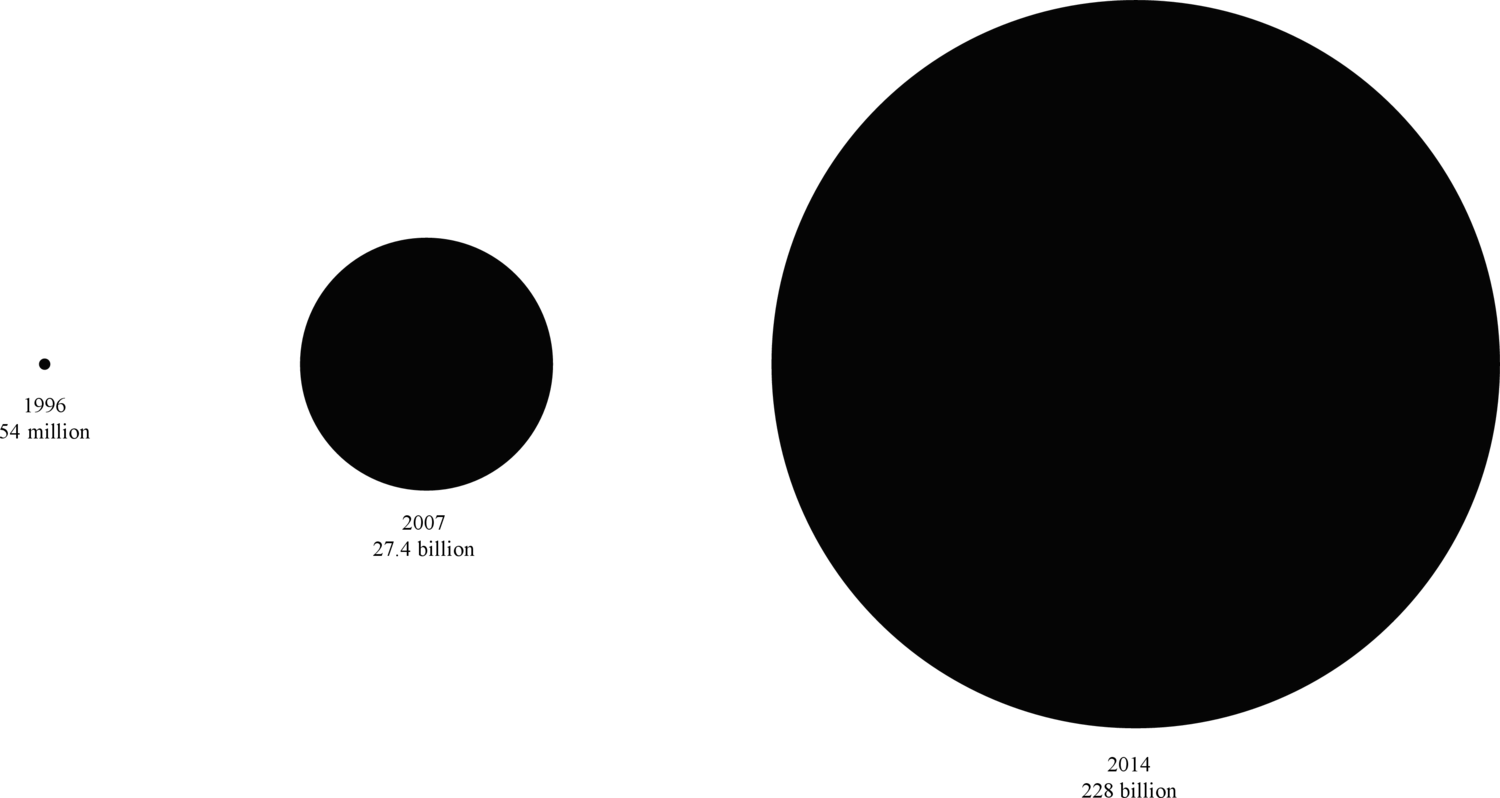
\includegraphics[width=0.98\columnwidth]{figures/Figure1_amountofdata/Figure1_amountofdata}
\caption{Theoretical growth of measurement data from electrical meters in commercial buildings in the USA in the last 20 years
\label{fig:datagrowth}%
}
\end{center}
\end{figure}

The analysis of the performance of buildings and the characterization of the building stock are necessary and, as discussed, quite tedious challenges in the building industry. Thus, a critical opportunity for the building industry is how these techniques can utilize the aforementioned explosion of detailed, temporal sources. 

\begin{itemize}
  \item \emph{If one has access to raw data from hundreds, or even thousands, of buildings, how can analysis be scaled in a robust way?}
  \item \emph{How can these data be used to inform the larger research community about the phenomenon occurring in the actual building stock?}
  \item \emph{What characteristic data about buildings can be inferred from these sources?}
\end{itemize} 

Non-residential buildings are the focus of this analysis as they are unique and complex in their energy-consuming systems. This decision was designed to limit the scope to a subset of the building industry that is under-researched as compared to residential buildings.

\section{A Framework for Automated Characterization of Large Numbers of Non-Residential Buildings}
\label{sec:frameworkforanalysis}

This thesis develops a framework to investigate which characteristics of whole building electrical meter data are most indicative of various meta-data about buildings amongst large collections of commercial buildings. This structure is designed to \emph{screen} electrical meter data for insight on the path towards deeper data analysis. The screening nature of the process is motivated by the scalability challenges previously outlined. An initial component in the methodology was a series of case study interviews and data collection processes to survey field data from numerous buildings around the world. Two phases were then applied to the collected data. The first was to use a library of temporal feature extraction techniques for the purpose of retrieving various behavior from whole building electrical sensor data in a relatively fast and unsupervised fashion. The second process utilizes these features in classification models to determine the accuracy of predicting various meta-data about each building. The classification aspect of the process is designed primarily to establish the importance of the input variables in their ability to characterize various behavior. Several meta-data are targeted to test this framework such as building use type, performance class, and operational strategy. These objectives were chosen as they represent steps in the direction of benchmarking, diagnostics, retrofit analysis, and other types of building performance analysis techniques. 

\section{Research Questions}
The primary question addressed through this research is:
\begin{itemize}
\item How accurately can the meta-data about a building be characterized through the analysis of raw hourly or sub-hourly, whole building electrical meter data? 
\end{itemize}

This question is dissected into several more specific parts:
\begin{itemize}
\item Which temporal features are most accurate in classifying the primary use-type, performance class, and operational strategy of a building?
\item Can temporal features be used to better benchmark buildings by signifying how \emph{well a building fits within its designated use-type class}?
\item Can temporal features be used to forecast whether an energy savings intervention measure will be successful or not?
\item What are the most appropriate parameter settings for various generalized temporal feature extraction techniques as applied to this context?
\item Is it effective or possible to implement such features across data from tens of thousands of buildings?
\end{itemize}

\section{Objectives}
The objectives of this research are as follows:
\begin{enumerate}
\item Consolidate and curate a set of feature extraction techniques from various research domains that automatically extract characteristic information from raw, temporal data
\item Extend these feature sets to include pattern recognition approaches that capture more information through characterizing usage patterns
\item Deploy these features on a test data set of 507 buildings to quantify the ability to characterize building use type, in-class performance, and operations types
\item Deploy a subset of features on a data set of approximately 1,600 buildings to test the ability to predict whether an energy-savings measure implementation will be a success 
\end{enumerate}

\section{Organization of the Thesis}
\label{sec:organization}

The remainder of this thesis is organized as follows. The research context of contemporary statistical learning and visual analytics techniques as applied to building performance is reviewed in Section \ref{sec:litreview}. This section has a special focus on unsupervised learning techniques as they are a strong basis for many of the temporal features extracted. Section \ref{sec:methodology} provides an overview of the two steps in the framework as well as the process of collecting data and insight from a series of case studies from around the world. Data from over 1200 buildings was collected on-site or through various open web portals and 507 were selected for further analysis. Sections \ref{sec:statisticsfeatures}-\ref{sec:patternbasedfeatures} provide in-depth overviews of each category of the temporal mining techniques implemented on the case study buildings, including explanatory visualizations of the range of values across the tested time range. Section \ref{sec:characterization} discusses the use of these features for the characterization of objectives such as predicting building use type, performance class, and operations type. Section \ref{sec:scalability} focuses on the use of a subset of temporal features in the industry classification and prediction of energy savings measures of close to 10,000 buildings with AMI data available. Finally, Section \ref{sec:conclusion} provides concluding remarks to understand the overall results of the thesis and future directions to pursue using the outlined techniques.                              % include 
\chapter{Research Context: Statistical Learning and Visual Analytics of Building Data}
\label{sec:litreview}

% \color{green} insert a long introduction as to why unsupervised techniques and visual analytics are necessary to this thesis}
This section gives an extensive overview of the techniques developed to extract automatically information from raw data to meet the scalability challenge. This content is developed as a publication submitted to the Renewable and Sustainable Energy Reviews Journal \citep{miller_review_????}. The domains and range of techniques reviewed go beyond the scope of this dissertation. It considers a range of applications and objectives beyond the presented framework and research questions. The purpose of this effort is to set a wider context for understanding and discuss broader challenges and opportunities.

Researchers from several domains have developed methods of extracting insight from raw data from the built environment. Often these methods fall into the category of statistical learning, often from unsupervised learning. Methods from this sub-domain of machine learning are advantageous due to their ability to characterize measured or simulated performance data quickly with less analyst intervention, meta-data, and ground truth labeled data. In this section, a review of previous work in analytics methods is covered by the categories of smart meter analytics, portfolio analytics, operations and control, and anomaly detection for buildings.

\section{Previous Reviews of Data Analytics in Buildings}
\label{sec:previousreviews}

Various reviews have been completed that overlap with this section. Most of them are designed to focus on a single core domain of research; the main two areas are building operations analysis and smart grid optimization. One of the earliest reviews of artificial intelligence techniques for buildings was completed in 2003 by Krarti and covered both supervised and unsupervised methods \citep{krarti_overview_2003}. Dounis updated this work and focused on outlining specific techniques in detail \citep{dounis_artificial_2010}.  Reddy's seminal book about a large variety of analysis techniques for energy engineers includes chapters on clustering and unsupervised methods specifically \citep{reddy_applied_2011}. Lee et al. describe a variety of retrofit analysis toolkits which incorporate unsupervised and visual analytics approaches in a practical sense \citep{lee_energy_2015}. Ioannidis et al. created a large ontology of data mining and visual analytics for building performance analysis, however with a strong focus on the techniques and not examples of works using them \citep{ioannidis_big_2015}. From the utility and power grid side, Morias et al. created a general overview of various data mining techniques as focused on power distribution systems \citep{morais_overview_2009}. Chicco covered clustering methods specifically focused on load profiling tasks \citep{chicco_overview_2012}. Zhou et al. included the concept of customer load classification  \citep{zhou_review_2013}.\\

\section{Overview of Publications}
\label{Overview}
The work for this section was created through a selection of unsupervised analytics categories outlined by authoritative sources from the machine learning community \citep{hastie_elements_2009,james_introduction_2013,duda_pattern_2012,mirkin_clustering:_2012}. The groups selected are clustering, novelty detection, motif and discord detection, and rule extraction. The field of visual analytics was added to these groups to cover the presentation layer of many of these types of techniques. An initial search of publications was then selected for inclusion through a Google Scholar search of the combination of the method categories and the terms ``building energy'', ``building performance analysis'', and ``building energy analysis''. From this initial list of publications, a set of application categories and sub-categories was developed as seen in Figure \ref{fig:categoriespie}. A more detailed search of each application class was then completed to account for the unique analytics techniques used in those domains. Only publications with a majority of the focus on utilization of unsupervised techniques and with a focus only on non-residential buildings are reviewed. Only works completed since 2005 are included to discuss only the most contemporary work and due to the relatively recent development of most of the techniques examined. A cutoff date of April 1, 2016, is applied for inclusions of publications in this review.

\begin{figure}[ht!]
\begin{center}
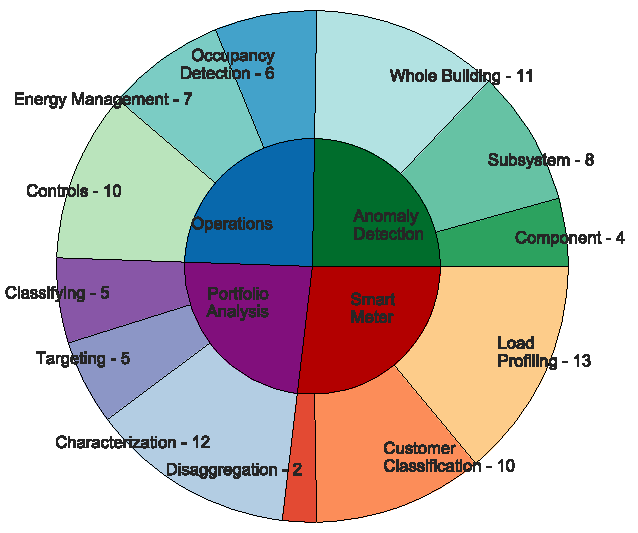
\includegraphics[width=0.7\columnwidth]{figures/PieChart_resized/PieChart_resized}
\caption{Categories and sub-categories (including number of publications) of building performance analysis applications of statistical learning and visual analytics
\label{fig:categoriespie}%
}
\end{center}
\end{figure}

\subsection{Research Sectors}
\label{sec:subsectors}

Figure \ref{fig:yearbreakdown} illustrates the breakdown of publications based on the year published since 2005. They are further divided into four broad research domains: building energy analysis, building simulation, computer science and electrical engineering. These research field categories were subjectively determined for each paper through evaluating a combination of which university department the authors were from and in which publication the study was published. Building energy analysis pertains to researchers who predominantly focus on measured data analysis from buildings while simulation experts research forward modeling and simulation of building and urban systems. Both fields of study most often exist within architecture or mechanical engineering departments. Electrical engineering and computer science are two well-established domains and exist in their departments. It is noticed that there is a gradual increase in the number of publications over the last ten years with electrical engineering and building energy analysis being the most common in the first few years and computer science and building simulation picking up since 2008. 

\begin{figure}[ht!]
\begin{center}
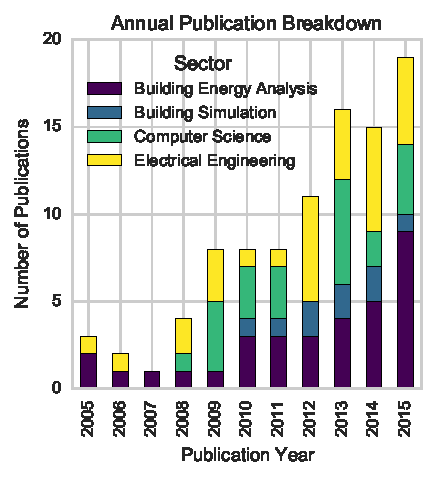
\includegraphics[width=0.5599999999999999\columnwidth]{figures/PublicationYear/PublicationYear}
\caption{Breakdown of publications by year published and research domain
\label{fig:yearbreakdown}%
}
\end{center}
\end{figure}

\subsection{Publications Venues}
This section analyzes the prevalence of certain publication venues within this section. Figure \ref{fig:journalbreakdown} illustrates the breakdown of the publication venues represented. The Energy and Buildings Journal from the building energy analysis domain dominates this list with 17 articles. Building simulation and energy analysis research domains publish most often in this journal as well as Applied Energy and Energy Efficiency. Several IEEE conferences and journals are also dominant as most of the papers from the electrical engineering domain are in these venues.

\begin{figure}[ht!]
\begin{center}
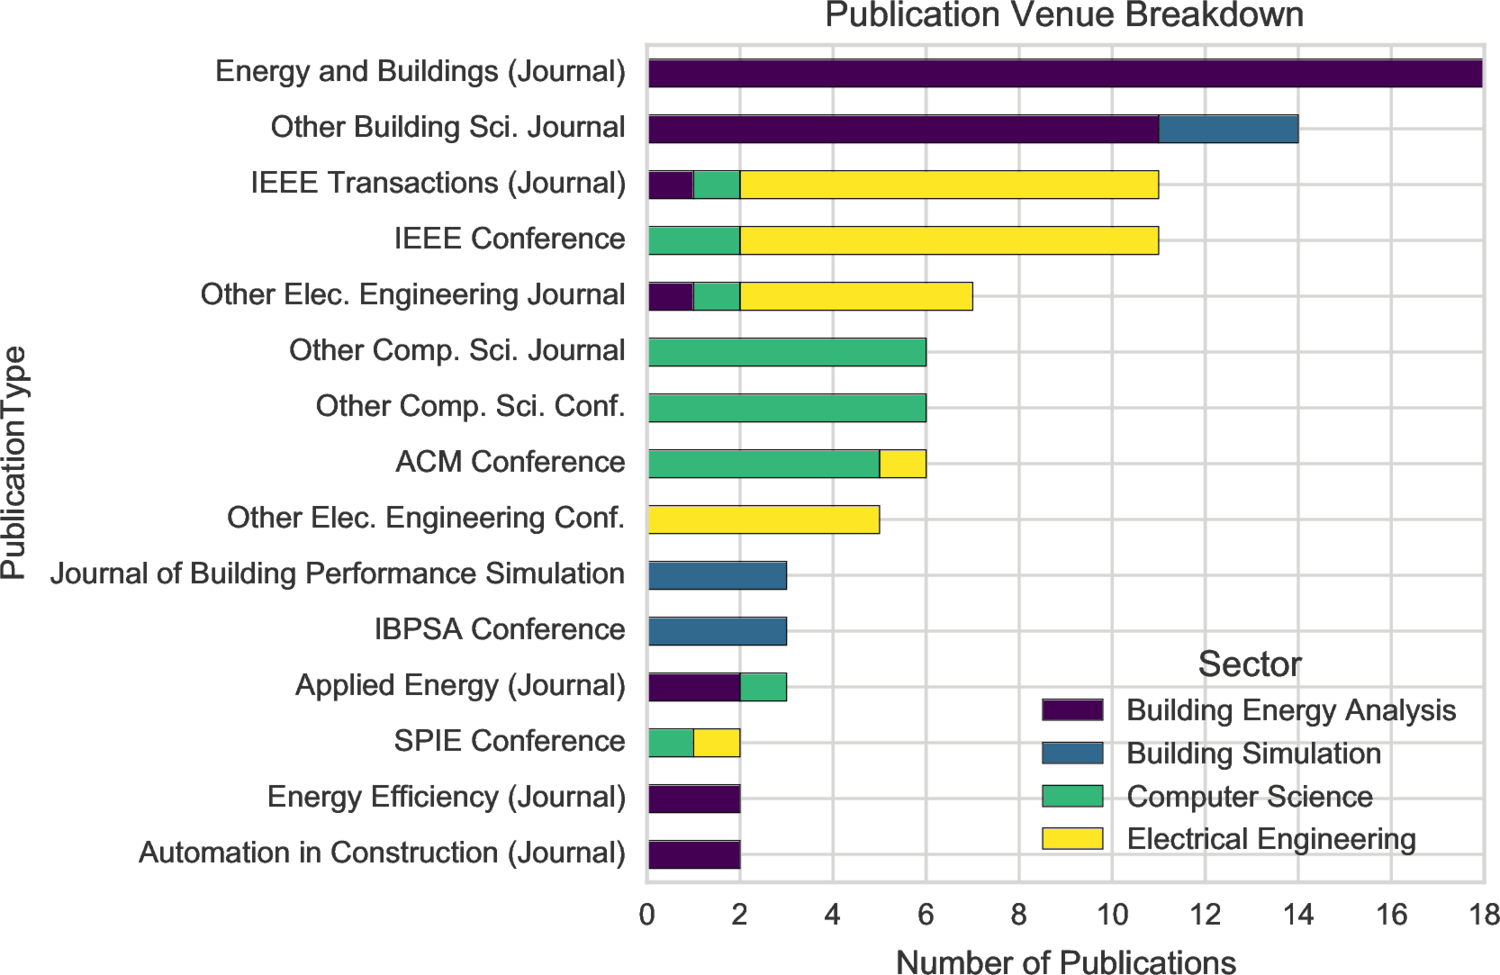
\includegraphics[width=1\columnwidth]{figures/PublicationVenues/PublicationVenues}
\caption{Breakdown of publications by publication type and research domain
\label{fig:journalbreakdown}%
}
\end{center}
\end{figure}

\section{Smart Meter Analytics}
\label{SmartMeter}
Advanced Metering Infrastructure (AMI), also known as smart meter systems, is a network of energy meters, most often focused on the electrical power measurement of a whole building. These systems are implemented and utilized by electrical utility providers. Conventional metering infrastructure only facilitates monthly data collection for billing purposes, while the new AMI framework allows for sub-hourly electrical demand readings. These data are primarily used for demand characterization and billing, however, many additional uses are being discovered. A wide-range of studies have been completed in recent years to focus on a range of issues related to automatically extracting information from these data using unsupervised techniques. In this section, three sub-categories of application are discussed: load profiling, account classification, and disaggregation.

\subsection{Load Profiling}
Load profiling is the process of grouping temporal subsequences of measured energy data for the purpose of characterizing the typical behavior of an individual customer. It involves time-series clustering and feature extraction. Chicco et al. provide an original example in our review of this process using support vector machine clustering \citep{chicco_support_2009}. Gullo et al. and R\"as\"anen et al. took the process further by introducing a framework of various clustering procedures that were implemented on case studies \citep{gullo_low-voltage_2009,rasanen_feature-based_2009}. Ramos et al., Iglesias et al., and Panapakidis et al. tested various conventional and new clustering methods and similarity metrics to determine those most applicable to electrical load profiling \citep{iglesias_analysis_2013,ramos_typical_2012,panapakidis_evaluation_2015}. Chicco et al. explored new clustering techniques based on ant colony grouping while Pan et al. discovered the use of kernel PCA for the same purpose \citep{chicco_electrical_2013,pan_kernel-based_2015}. Several groups of researchers such as Lavin and Klabjan and Green et al. have found efficient use in using the core K-Means clustering algorithm for load profiling \citep{lavin_clustering_2014,green_divide_2014}. Shahzadeh et al. discussed the use of profiling as applied to forecast accuracy of temporal data \citep{shahzadeh_improving_2015}. Two studies diverge from the standard profile development using clustering paradigm. The first is by De Silva et al. who uses Incremental Summarization and Pattern Characterization (ISPC) instead of clustering to find load profiles \citep{de_silva_data_2011}. The other is the visual analytics-based approach of creating a smart meter analytics dashboard by Nezhad et al. to set up and inspect typical load profiles \citep{jarrah_nezhad_smartd:_2014}.

\subsection{Customer Classification}
Automated account classification is the next sub-category that utilizes unsupervised learning techniques within the smart meter domain. These methods often employ load profile clustering as a first step but differentiate themselves in using those features to classify accounts, or buildings, that fit within various categories. Therefore, account classification is a type of manual semi-supervised analysis utilizing load profiling as a basis. The study by Figueiredo et al. harnessed K-Means and a labeled sample from accounts in Portugal to showcase this concept \citep{figueiredo_electric_2005}. Verdu et al. and R\"as\"anen et al. applied self-organizing maps (SOM) to accomplish a similar study that classifies accounts according to the applicability of several demand response scenarios \citep{verdu_classification_2006,rasanen_reducing_2008}. Vale et al. give an overview of a general data mining framework focused on characterizing customers \citep{vale_data_2009}. Florita et al. diverge from the use of measured data by creating a massive amount of simulation data of load profiles to quantify energy storage applications for the power grid \citep{florita_classification_2012}. Fagiani et al. use Markov Model novelty detection to automatically classify customers who potentially have leakage or waste issues \citep{fagiani_novelty_2015}. Cakmak et al. and Liu et al. test new visual analytics techniques within more holistic analysis framework for analyzing customers \citep{cakmak_new_2014,liu_smas:_2015}. Borgeson used various clustering and occupancy detection techniques to analyze a large AMI data set from California \citep{borgeson_targeted_2013}. Bidoki et al. tested various clustering techniques to evaluate applicability for customer classification \citep{bidoki_evaluating_2010}. A recent study in Korea develops a new clustering method for segmenting customers to analyze demand response incentives \citep{jang_variability_2016}.

\subsection{Disaggregation}
The last area of smart meter data analysis is the field of meter disaggregation. Disaggregation attempts decompose a measurement signal from a high level reading to the individual loads being measured. This domain is well-researched from a supervised model perspective but recent attempts at unsupervised, pattern-based disaggregation were developed to facilitate implementation on unlabeled smart meter data. Shao et al. use Dirichlet Process Gaussian Mixture Models to find and disaggregate patterns in sub-hourly meter data \citep{shao_temporal_2013}. Reinhardt and Koessler use a version of symbolic aggregate approximation (SAX) to extract and identify disaggregated patterns for the purpose of prediction \citep{reinhardt_powersax:_2014}. These studies are also unique in that few of the disaggregation studies focus on commercial buildings as opposed to residential buildings.

\section{Portfolio Analytics}
\label{PortfolioAnalytics}

Portfolio analysis is a domain in which a large group of buildings, often located in the same geographical area or owned or managed by the same entity, are analyzed for the purpose of managing or optimizing the group as a whole. Each subsection covers the publications reviewed in this domain that fall into three categories: characterization, classification, and targeting.

\subsection{Characterization}
Publications that address the characterization of a portfolio of buildings include unsupervised techniques meant to evaluate and visualize the range of behaviors and performance of the group. A majority of the techniques utilized are either clustering or visual analytics that provide a model of exploratory analysis that enable further steps. Seem produced an influential study that extracts days of the week with similar consumption profiles \citep{seem_pattern_2005}. Further clustering work was completed by An et al. to estimate thermal parameters of a portfolio of buildings \citep{an_estimation_2012}. Lam et al. used Principal Component Analysis to extract information about a group of office buildings \citep{lam_principal_2008}. Approaches focused on visual analytics and dashboards were completed by Agarwal et al., Lehrer, and Lehrer and Vasudev \citep{agarwal_energy_2009,lehrer_research_2009,lehrer_visualizing_2011}. Granderson et al. completed a case study-based evaluation of energy information systems, in which some methods combine some unsupervised approaches with visualization \citep{granderson_building_2010}. Diong et al. completed a case study as well focused on a specific energy information system implementation  \citep{diong_establishing_2015}. Mor\'an et al. and Georgescu and Mezic developed hybrid methods that employed visual continuous maps and Koopman Operator methods respectively to visualize portfolio consumption\citep{moran_analysis_2013,georgescu_site-level_2014}. Miller et al. completed two studies focused on the use of screening techniques to automatically extract diurnal patterns from performance data and use those patterns to characterize the consumption of a portfolio of buildings  \citep{miller_forensically_2015,miller_automated_2015}. Yarbrogh et al. used visual analytics techniques to analyze peak demand on a university campus \citep{yarbrough_visualizing_2015}.

\subsection{Classification}
The concept of classifying buildings within a portfolio supplements the characterization techniques by assigning individual buildings to subgroups of relative performance for the purpose of benchmarking or decision-making. Santamouris et al. produced a report using clustering and classification to assign schools in Greece to subgroups of similar performance \citep{santamouris_using_2007}. Nikolaou et al. and Pieri et al. further extended this type of work to office buildings and hotels\citep{nikolaou_application_2012,pieri_identifying_2015}. Heidarinejad et al. released an analysis of clustered simulation data to classify LEED-certified office buildings \citep{heidarinejad_cluster_2014}. Ploennigs et al. created a platform for monitoring, diagnosing and classifying buildings and operational behavior within a portfolio to quickly visualizing the outputs \citep{ploennigs_e2-diagnoser:_2014}.

\subsection{Targeting}
Targeting is a concept that builds upon characterization and classification to identify specific buildings or measures to be implemented in a portfolio to improve performance. These publications are differentiated in that specific measures are identified in the analysis. Sedano et al. use Cooperative Maximum-Likelihood amongst other techniques to evaluate the thermal insulation performance of buildings \citep{sedano_improving_2009}. Gaitani et al. used PCA and clustering to target heating efficiency in school buildings \citep{gaitani_using_2010}. Bellala et al. used various methods to find lighting energy savings on a campus of a large organization \citep{bellala_towards_2011}. Petcharat et al. also found lighting energy savings in a group of buildings \citep{petcharat_assessment_2012}. Cabrera and Zareipour used data association rules to complete a similar study to find wasteful patterns \citep{cabrera_data_2013}. Geyer et al.  and Schlueter et al. test various clustering strategies to group different buildings within a Swiss alpine village according to their applicability for retrofit interventions \citep{geyer_application_2016} and thermal micro-grid feasibility \citep{schlueter_analysis_2016}.

\section{Operations, Optimization, and Controls}
\label{Operations}
Unsupervised techniques focused on individual buildings themselves are placed in the category for building operations, optimization, and control. This class contains the largest number of publications, and it incorporates a wider range of applications. It is differentiated from Section \ref{AnomalyDetection} in that the applications are not as focused on detecting and fixing the anomalous behavior. This section evaluates publications within the sub-categories of occupancy detection, retrofit analysis, controls, and energy management. 

\subsection{Occupancy Detection}
Occupancy detection using unsupervised techniques infers human presence in a non-residential building without a labeled ground truth dataset or as part of a semi-supervised approach using a subset of labeled data. This occupancy detection is then used for analysis or as inputs for control of systems. Augello et al. used multiple techniques to infer occupant presence on a campus in Italy \citep{augello_sensor_2011}. Dong and Lam used Hidden Markov Models to detect occupancy patterns that were then used in a simulation \citep{dong_building_2011}. Thanayankizil et al. developed a concept called Context Profiling in which occupancy was detected temporally and spatially \citep{thanayankizil_softgreen:_2012}. Mansur et al. used clustering to detect occupancy patterns from sensor data \citep{mansur_learning_2015}. The newest studies by Adamopoulou et al. and D'Oca and Hong use a range of techniques to extract rules related to occupancy \citep{adamopoulou_context-aware_2015,doca_occupancy_2015}. A recent study using wavelets illustrates the correlation of occupancy with actual energy consumption \citep{ahn_correlation_2016}.

\subsection{Controls}
Controls optimization is an enduring field of study aimed at creating a state of the best operation and energy performance for a building system such as heating, cooling, ventilation or lighting. Kusiak and Song created a means of optimally controlling a heating plant with clustering as a key step \citep{kusiak_clustering-based_2008}. Patnaik et al. completed studies focused on using motif detection to find modes of chilled water plant operation that proved most optimal \citep{patnaik_data_2010,patnaik_sustainable_2009}. Hao et al. built upon these concepts to create a visual analytics tool to investigate these motifs \citep{hao_visualizing_2011}. May-Ostendorp et al. used rule extraction as a means of enhancing a model-predictive control process of mixed-mode systems \citep{may-ostendorp_model-predictive_2011,may-ostendorp_extraction_2013}. Bogen et al. used clustering to detect usage patterns for building control system evaluation \citep{bogen_evaluating_2013}. Fan et al. used clustering to enhance chiller power prediction with the ultimate goal of control optimization \citep{fan_prediction_2013}. Hong et al. used Empirical Mode Decomposition to spatially optimize the placement of sensors in a building \citep{hong_towards_2013}. Domahidi et al. used support vector machines (SVM) to extract optimized rules for supervisory control \citep{domahidi_learning_2014}. Habib and Zucker use SAX to identify common motifs of an absorption chiller for the purpose of characterization and control \citep{habib_finding_2015}.

\subsection{Energy Management}
Energy management and analysis of an individual building using unsupervised techniques is becoming common due to the increasing amounts of raw building management (BMS) and energy management system (EMS) data. Users of these techniques are often facilities management professionals or consultants who undertake the process to understand how the building is consuming energy. Duarte et al. use visual analytics to process data from an EMS along with various pre-processing techniques \citep{duarte_prioritizing_2011}. Lange et al. created two overview studies focused spatiotemporal visualization of building performance data and its interpretation in various case studies \citep{lange_energy_2012,lange_discovering_2013}. Gayeski et al. completed a recent survey of operations professionals on their use of graphical interfaces of BMS and EMS dashboards \citep{gayeski_data_2015}. Outside of the visual analytics realm, Fan et al., Xiao and Fan, and Yu et al. completed studies of an entire data mining using framework using data association rules to improve operational performance \citep{fan_temporal_2015,xiao_data_2014,yu_extracting_2013}.

\section{Anomaly Detection}
\label{AnomalyDetection}
Anomaly detection for buildings focuses on the detection and diagnostics of problems occurring within a building, its subsystems, and components. This field is most often focuses on the use of novelty detection or clustering approaches to find anomalous behavior. The sub-categories for this section are divided according to the spatial hierarchy of systems within a building; the highest level is whole building consumption, down to the subsystems such as heating, cooling or lighting and then to the individual components of those systems. 

\subsection{Whole Building}
Whole building anomaly detection uses the electricity or heating and cooling energy supply in coming to a building to determine sub-sequences of poor performance. This category is complimentary to many of the Smart Meter solutions as they both focus on the use of a single data stream for a building. Seem had an early work again in this category with his work in using novelty detection to find abnormal days of consumption in buildings \citep{seem_using_2006}. Liu et al. used classification and regression trees (CART) \citep{liu_method_2010} and Wrinch et al. use frequency domain analysis for the same purpose \citep{wrinch_anomaly_2012}. Jacob et al. utilized hierarchical clustering to use as variables in regression models for whole building monitoring \citep{jacob_black-box_2010}. Fontugne et al. created a process known as the \emph{Strip, Bind, and Search} method to automatically uncover misbehavior from the whole building level and subsequently detects the source of the anomaly \citep{fontugne_strip_2013}. Janetzko et al. developed a visual analytics platform to highlight anomalous behavior in power meter data \citep{janetzko_anomaly_2013}. Chou and Telaga created a hybrid whole building anomaly detection process using K-means \citep{chou_real-time_2014}. Ploennigs et al. and Chen et al. created similar systems that use generalized additive models (GAM) \citep{ploennigs_exploiting_2013,chen_statistical_2014}. In the most recent work, Capozzoli et al. and Fan et al. use various techniques as part of a framework to detect and diagnose performance problems \citep{capozzoli_fault_2015,fan_framework_2015}. 

\subsection{Subsystems}
Subsystem anomaly detection focuses on the use of a broader data set to detect and diagnose faults from a lower level. Yoshida et al. provided a semi-supervised approach that seeks to determine which variables within a building are most influential in contributing to overall building performance  \citep{yoshida_identification_2008}. Wang et al. use PCA to diagnose sensor failures \citep{wang_system-level_2010}. Forlines and Wittenberg visualized multi-dimensional data using what they call the Wakame diagram \citep{forlines_wakame:_2010}. Linda et al. and Wijayasekara et al. use various techniques to diagnose system faults and visualize them spatially \citep{linda_computational_2012,wijayasekara_mining_2014}. Le Cam et al. use PCA to create inverse models to detect problems in HVAC systems \citep{le_cam_application_2014}. Li and Wen created a similar process using PCA in conjunction with wavelet transform \citep{li_model-based_2014}. Sun et al. used data association rules to create fault detection thresholds for finding anomalies \citep{sun_efficient_2015}.

\subsection{Components}
Component level anomaly detection is a bottom-up fault detection approach that focuses on determining faults in individual equipment. Wang and Cui use PCA to detect component faults in chilled water plants  \citep{wang_sensor-fault_2005}. Yu et al. and Fontugne et al. both compliment their work at the whole building level to find associated component performance anomalies automatically \citep{yu_novel_2012,fontugne_mining_2013}. Zhu et al. use wavelets to diagnose issues in air handling units (AHU) \citep{zhu_fault_2012}.

\section{Discussion}
\label{discussion}
Several challenges facing the use of unsupervised machine learning in building performance were uncovered through this process of review. The first relates to the effect of several traditional research sectors exploring techniques targeted on the improvement of building performance. It was found that different sets of terminology are used to describe similar concepts. For example, in the building energy analysis field, the term \emph{fault} (such as \citep{zhu_fault_2012}) is used to describe a situation that is similar to what is labeled an \emph{anomaly} in the data mining domain (such as \citep{fontugne_mining_2013}). Thus, discussions between these fields are restrained and completing a review of knowledge is difficult.

A critical issue related to differences in domains is the inconsistency of success objectives. Often individual papers would discuss the accuracy or efficiency of the algorithm or technical process itself (such as \citep{iglesias_analysis_2013}), while others focused exclusively on the end results of the evaluation such as how much energy was saved (such as \citep{seem_using_2006}). Several examples publications successfully address both types of issues. For example, Ploennings et al. published studies which both addressed the applicability of generalized additive models and discussed their implementation in a platform that is applied to real buildings \citep{ploennigs_exploiting_2013,ploennigs_e2-diagnoser:_2014}. Researchers should strive to optimize in both the theoretical and practical domains to have the most impact on real buildings.

Another observation relates to the lack of easy reproducibility amongst studies. Reproducibility provides the ability for a third-party researcher to easily recreate the results of a study through a release of the data or code developed. Recent prominent articles have outlined the importance of reproducibility in science \citep{_journals_2014} and the sharing of data and code to enhance this pursuit \citep{_code_2014}. The biomedical sciences research community is leading the way in this effort; editors from over 30 major journals, funding agency representatives, and scientific leaders from that field created guidelines for the enhancement of reproducibility \citep{_journals_2014}. Research from the building performance analysis community should follow this lead, specifically on machine learning and other types of empirical analysis.

Another challenge discovered is the lack of clarity regarding which is the optimal technique for each application. For example, a number of studies were completed to test the ability of clustering techniques to group similar daily load profiles \citep{chicco_support_2009,de_silva_data_2011,green_divide_2014,gullo_low-voltage_2009,lavin_clustering_2014,ramos_typical_2012,shahzadeh_improving_2015}. A researcher or analyst who is searching for the best technique can see a survey of implementations through these publications; however, it's hard for them to be compared against each other as each utilizes a different data set and incorporates different methodologies. An explanation of the amount of effort needed to implement a technique is missing in most studies as well. For example, to implement a certain algorithm on a potential use-case or data set, an analyst is interested in which parameters need to be tuned, what labeled ground truth data should be gathered, and what expertise is necessary for understanding and implementation. This lack of comparison stifles the ability to make conclusions about the efficiency, interpretability, and appropriateness of use of each algorithm. 

This dissertation seeks to address each of these challenges through the development of a framework that bridges the gap between the building energy performance, computer science, and electrical engineering. This goal is accomplished through incorporation of many of the approaches and techniques found in this literature review on a large collected temporal data set from buildings. A library of techniques, both mainstream and newly developed, are implemented on these data. This library is implemented on a collected and open data set. These techniques and data are to be shared with a wider audience through various means of reproducible research to be outlined in the methodology and conclusion sections. 
 

% \subsection{Opportunities}
% To address the challenges related to interdisciplinary collaboration, an opportunity exists for better dialogue between the electrical engineering, computer science, and building performance and simulation analysis research communities through cross-disciplinary venues that encourage submission of works from all domains. Several publication venues were found that publish papers written by academics from diverse backgrounds. IEEE and ACM conferences, in particular, were found to be somewhat diverse as compared to other publication outlets. The further development of these avenues will create a more welcoming environment in which different disciplines can exchange terminology, objectives, and culture. 



% \subsection{}
% As mentioned in the introduction, the scope of this section extends beyond the proposed  This dissertation addresses this issue by integrating a vast array of temporal mining techniques from various sub-fields and putting them directly in the context of building performance analysis. This interdisciplinary approach has aspects related to techniques, but also objectives.

\chapter{Methodology}
\label{sec:methodology}

As discussed in Section \ref{sec:intro}, a two-step process is presented as a means of extracting knowledge from whole building electrical meters. Figure \ref{fig:framework} illustrates the intermediate steps in each of the phases.

The first step is to extract temporal features that produce quantitative data to describe various phenomenon occurring in the raw temporal data. This action is intended to transform the data into a more human-interpretable format and visualize the general patterns in the data. In this step, the data are extracted, cleaned, and processed with a library of temporal feature extraction techniques to differentiate various types of behavior. This library is outlined in Sections \ref{sec:statisticsfeatures}-\ref{sec:patternbasedfeatures}. These features are visualized using an aggregate heat map format that can be used evaluated according to expert intuition, comparison with design intent metrics, or with outlier detection. Section \ref{sec:temporalfeatureextraction} gives a more detailed definition of temporal features and how they're utilized in this study.

The second step is focused on the characterization of buildings using the temporal features according to several objectives. This step allows an analyst to understand the impact each feature has upon the discrimination of each objective. Five test objectives are implemented in this study: principal building use, performance class, operations strategy, general industry class, and energy savings measure success. One of the key outputs of this supervised learning process is the detection and discussion of what input features are \emph{most important} in predicting the various classes. This approach gives exploratory insight into what features are important in determining various characteristics of a particular building amongst a large set of its peers. These metadata are building blocks for many other techniques such as benchmarking, diagnostics and targeting. The motivation for choosing these particular objectives centers around the consistently available meta-data from the collected case study data and their relation to various other techniques in the building performance analysis domain. These topics are covered through qualitative discussion with several of the operations teams on the campuses where the data were collected and is discussed more thoroughly in Section \ref{sec:characterization}.

\begin{figure}[ht!]
\begin{center}
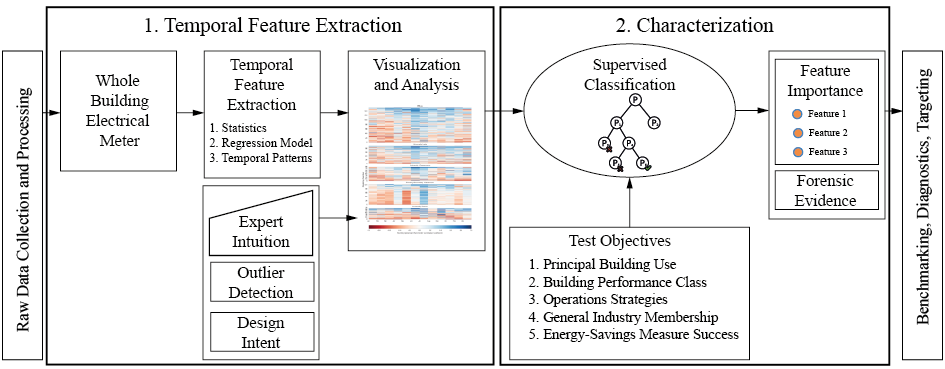
\includegraphics[width=1\columnwidth]{figures/process/FrameworkOverview3}
\caption{Overview of Data Screening Framework}
\label{fig:framework}%
}
\end{center}
\end{figure}


\section{Temporal Feature Extraction}
\label{sec:temporalfeatureextraction}

Feature extraction is an essential process of machine learning and is the means by which objects are described quantitatively in a way that algorithms can differentiate between different types or classes. Figure \ref{fig:convfeatures} illustrates a hierarchical node diagram of the features, or metadata, about a building that are often necessary to accumulate to perform conventional analysis from the literature. Much of these data are needed when creating an energy simulation model, when setting thresholds for automated fault detection and diagnostics, or benchmarking a building. When performing analysis on a single building, these meta-data might be easy to accumulate. However, when such a process is scaled across hundreds or potentially thousands of buildings, a collection of these data is not a trivial procedure. 
%This reality is reinforced through site interviews with campus-level energy managers as described later in this thesis.

%force chart data and viz in /Dropbox/04_ANALYSIS

\begin{figure}[ht!]
\begin{center}
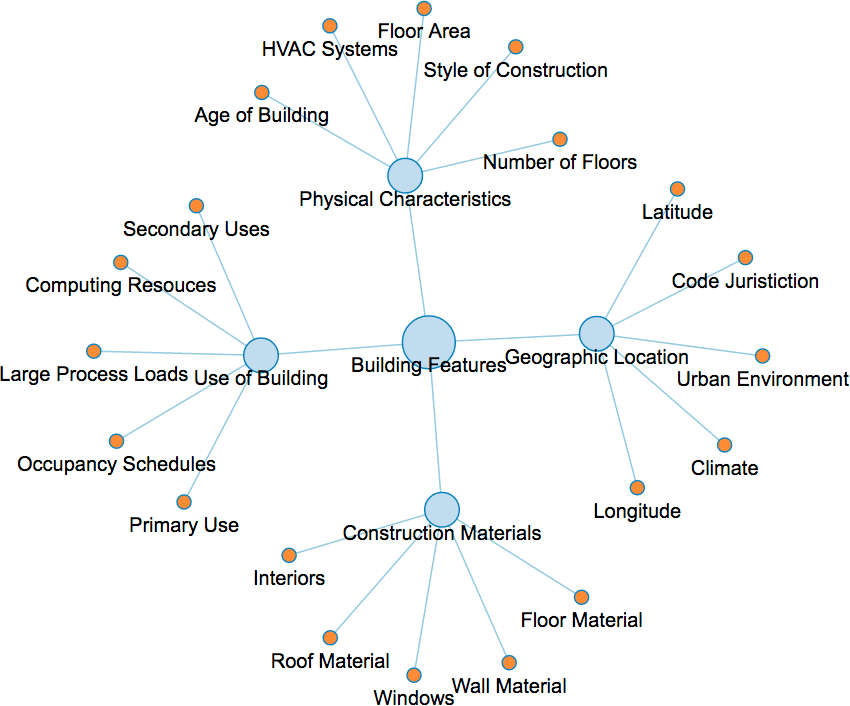
\includegraphics[width=0.7\columnwidth]{figures/TypicalFeatures/nontemporalforcechart}
\caption{Conventional features, or metadata, about a building
\label{fig:convfeatures}%
}
\end{center}
\end{figure}

Modern, whole building electrical meters measure and report raw, sub-hourly, time-stamped data. Significant amounts of essential information can be extracted from temporal data to characterize a commercial building. The harvest of this information can assist in the implementation of conventional analysis techniques, as inputs to classify or benchmark a building, or to predict whether a building is a good candidate for individual energy savings measures. To extract information solely from these sensors, new features can be created from these raw data. These features are designated as temporal as they summarize behavior occurring in time-series data. To illustrate the concept of temporal features qualitatively, Figure \ref{fig:electricalmeters_oneyear} shows four example hourly electrical meters from different buildings. Even to the untrained eye, these data streams show obvious differences in the way each building operates. Building A seems to be an extremely consistent consumer of energy across the entire year. There are no steady-state shifts in operation and seemingly no influence from outside factors. Qualitatively, this data stream can be thought of as \emph{consistent} or \emph{predictable}. Building B is similar in operation but has an obvious influence from an external factor in the summer months. It is safely assumed that the consumption of this building is weather-dependent, and it has some kind of cooling system. Building C illustrates behavior that has \emph{shifts} in consumption over the course of the year. This observation implies that this building has different schedules over the course of a year. Building D seems to have combinations of all of these attributes, with no obviously dominating phenomena. 


\begin{figure}[ht!]
\begin{center}
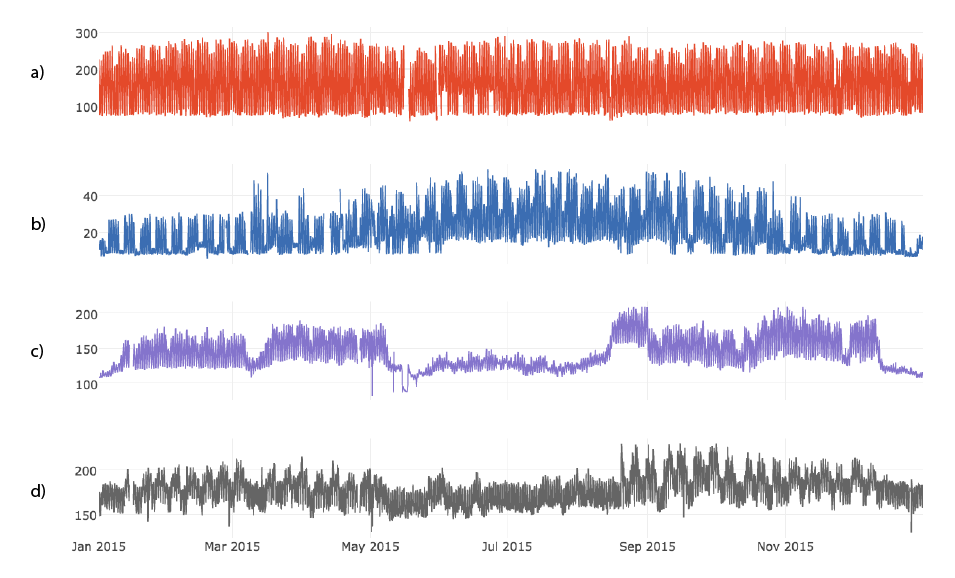
\includegraphics[width=0.98\columnwidth]{figures/temporal_metering_examples/temporal_metering_examples}
\caption{One year of example whole building electrical meter data that qualitatively exemplifying various temporal features
\label{fig:electricalmeters_oneyear}%
}
\end{center}
\end{figure}

Figure \ref{fig:electricalmeters_twoweeks} illustrates the same four buildings with the time range constrained to two weeks of data. Short-term temporal effects at the weekly and daily level are now observed. Building A still appears very consistent with a predictable daily cyclical pattern and a few variations around August 4 and 5. Building B exhibits similar behavior, but with noticeable weekend differences on Saturdays and Sundays. Building C has less observable daily patterns but has a trend upwards in the last five days of the time range. Building D, again, has a combination of these attributes.

\begin{figure}[ht!]
\begin{center}
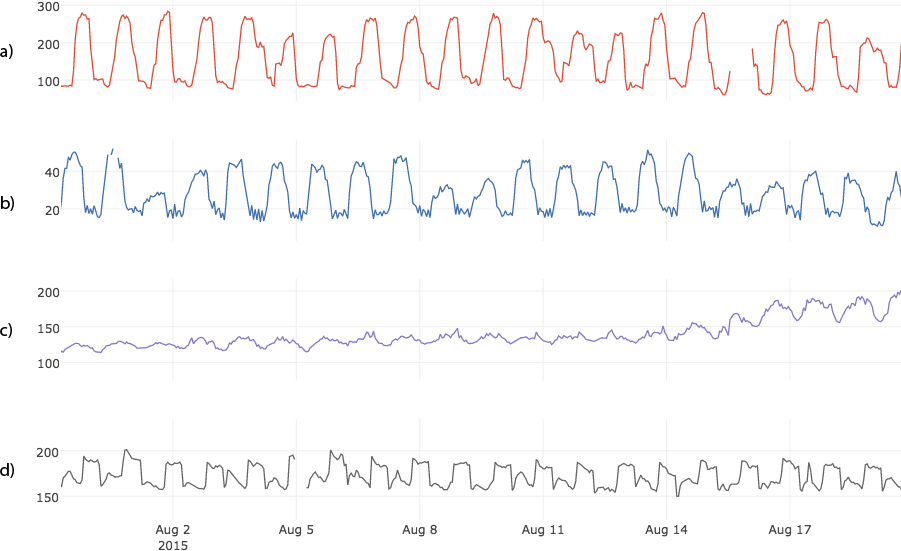
\includegraphics[width=0.98\columnwidth]{figures/temporal_metering_examples_zoomedin/temporal_metering_examples_zoomedin}
\caption{Two weeks of example whole building electrical meter data that qualitatively exemplifying various temporal features
\label{fig:electricalmeters_twoweeks}%
}
\end{center}
\end{figure}

The goal of temporal feature extraction and analysis is to use various techniques to convert all these \emph{qualitative} terms into a \emph{quantitative} domain. For example, the descriptor \emph{weather-dependency} can be quantified through the use of the Spearman rank order correlation coefficient with outdoor air temperature. Consistency or volatility of daily, weekly, or annual behavior can be quantified using various pattern recognition techniques. The primary focus of this study is to create and apply some temporal feature extraction techniques on commercial buildings for the purpose of characterization. Figure \ref{fig:temporalfeatures} illustrates the categories of temporal features created in this effort.

\begin{figure}[ht!]
\begin{center}
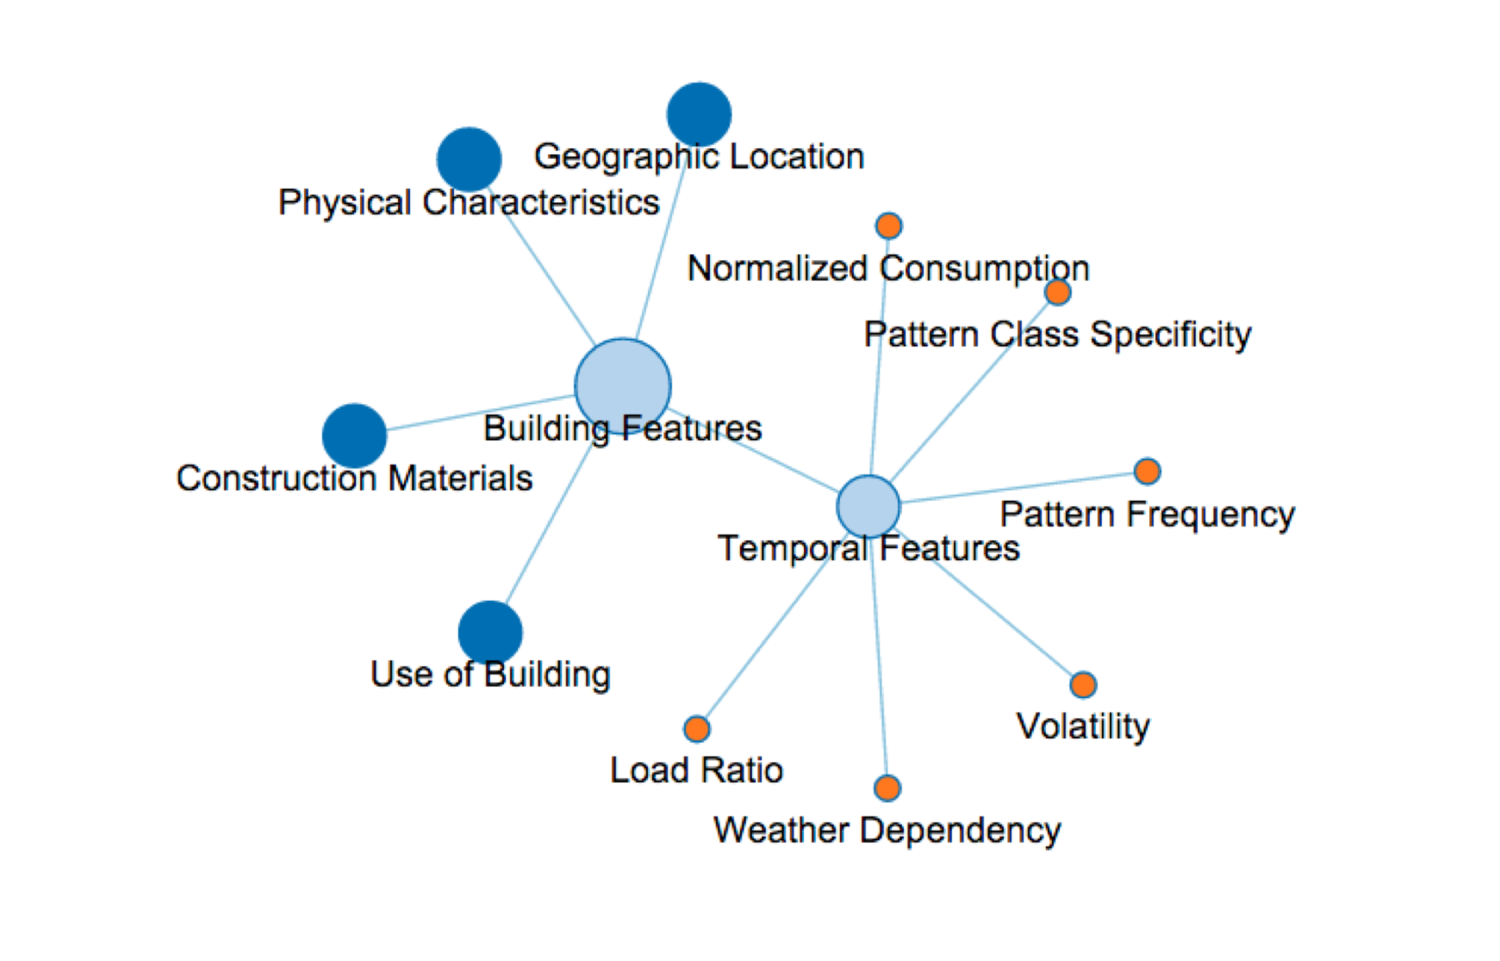
\includegraphics[width=0.7\columnwidth]{figures/TemporalFeatures/TemporalFeatures}
\caption{Temporal features extracted solely from raw sensor data
\label{fig:temporalfeatures}%
}
\end{center}
\end{figure}

Temporal features are aggregations of the behavior exhibited in time-series data. They are characteristics that summarize sensor data in a way to inform an analyst through visualization or to use as training data in a predictive classification or regression model. Feature extraction is a step in the process of machine learning and is a form of dimensionality reduction of data. This process seeks to quantify various qualitative behaviors. This section provides and overview of the categories of temporal features extracted from the case study building data, the methods used to implement them, and visualized examples of a selected subset of features manifest themselves over a time range. Table \ref{tab:featureoverview} gives an overview the temporal features outlined in this section.  A detailed list of the temporal features created in this Section can be found in Appendix A. 

\begin{table} 
    \begin{tabular}{| p{8cm} | p{6cm}  |}
        \hline
        \textbf{Feature Category} &  \textbf{General Description}\\ 
        \hline
        Statistics-based & Aggregations of time series data using mean, median, max, min, standard deviation \\ 
        \hline
        Regression model-based & Development of a predictive model using training data and using model parameters and outputs to describe the data \\ 
        \hline
        Pattern-based &  Extraction of frequent and useful daily, weekly, monthly, or long-term patterns\\ 
        \hline
    \end{tabular} 
    \caption{Overview of feature categories}
\end{table}
\label{tab:featureoverview}

\section{Characterization and Variable Importance}
\label{sec:variableimportance}

The primary goal of this dissertation is to get a better sense of what behavior in time-series sensor data is most characteristic of various \emph{types} of buildings. As mentioned in the introduction, if this meta-data can be discriminated, the process of characterizing a building can be automated. In this section, the process of using random forest classification models and the input variable importance feature.

For each objective, several steps are taken to predict each objective and then to investigate the influence of the input features on class differentiation:
\begin{enumerate}
\item A random forest classification model is built using subsets of the generated features to predict the objectives class
\item The classification model provides an indication of the ability of the temporal features in describing the class based on its accuracy
\item Input feature importance is calculated by the classification model for insight on what the most informative features are in predicting class
\item An in-depth analysis comparison of two of the classes within each objective is completed to explore further the attributes that characterize a building
\end{enumerate}

An overview of this process is found in Figure \ref{fig:char_process}. After the technical analysis of the ability for the features sets to characterize building use type, a discussion is presented for each subsection on the practical insight gained from this process from discussions with the case study participants outlined in Section \ref{sec:sitevisit}.

\begin{figure}[ht!]
\begin{center}
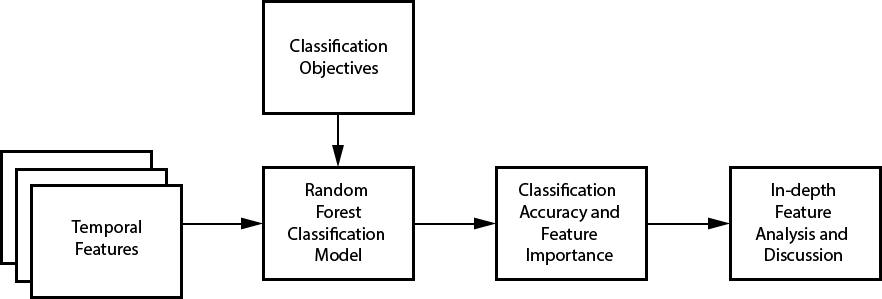
\includegraphics[width=0.98\columnwidth]{figures/characterization_process/characterization_process}
\caption{{Characterization process to investigate the ability for various features to describe the classification objectives
\label{fig:char_process}%
}}
\end{center}
\end{figure}

Random forest classification models were chosen based on their ability to model diverse and large data sets in a robust way \cite{Breiman}. These models use an ensemble of decision trees to predict various characteristic labels about each building based on its features. The literature describes decision trees as the "closest to meeting the requirements for serving as an off-the-shelf procedure for data mining" \cite{hastie_elements_2009}. Figure \ref{fig:decisiontree} illustrates an example of a decision tree using features to determine whether a patient is sick or healthy using two features \cite{Geurts_2009}. 


\begin{figure}[ht!]
\begin{center}
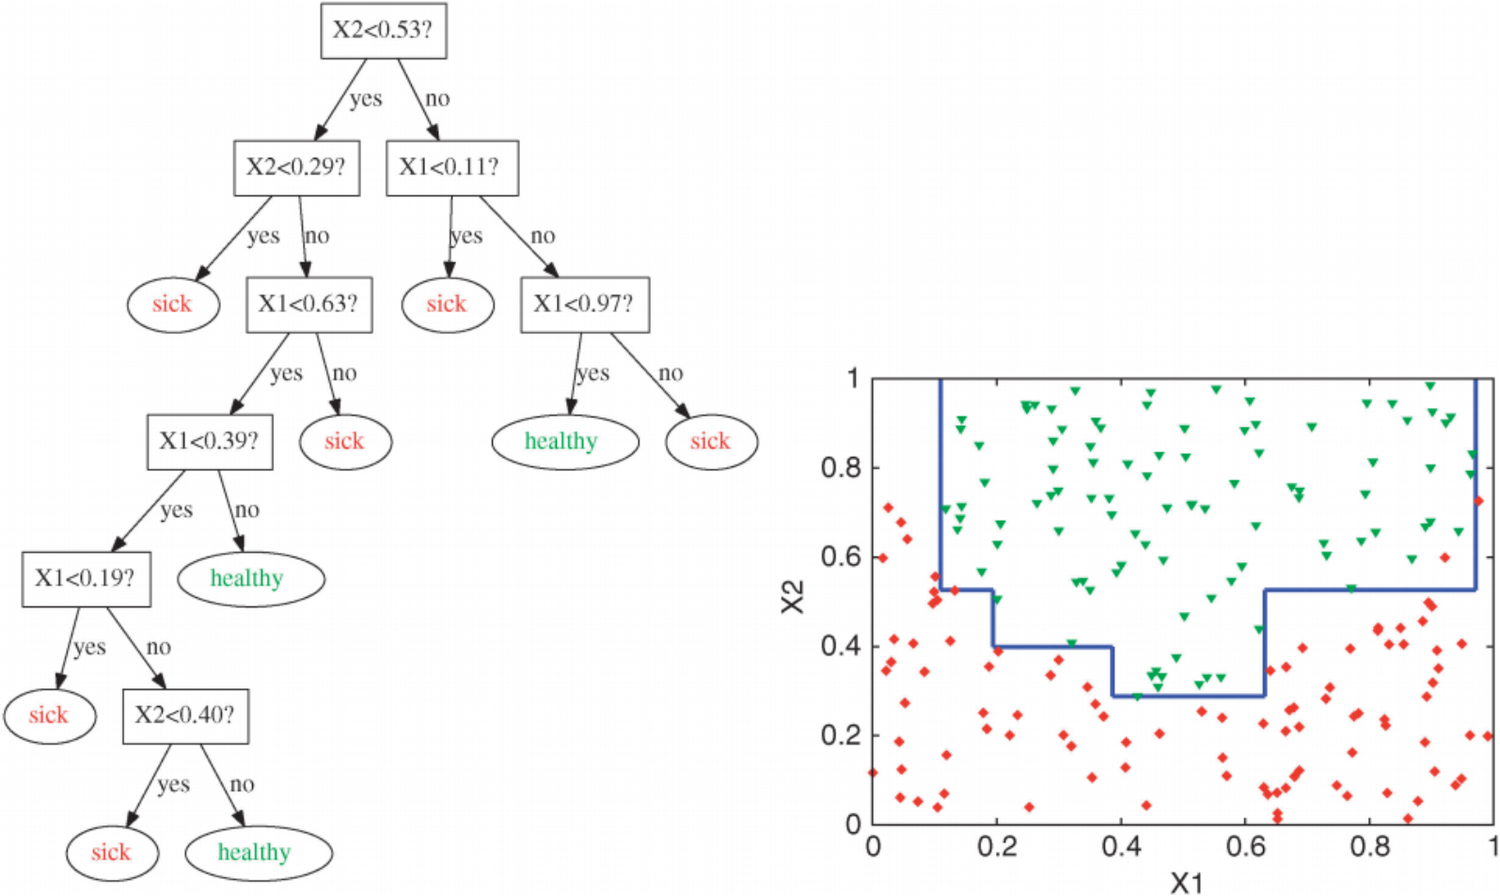
\includegraphics[width=1\columnwidth]{figures/CART_tree_titanic_survivors/decision_tree}
\caption{{An example of a decision tree (left) with the decision boundary for two features, $X1$ and $X2$ (right). Adaption with permission from \cite{Geurts_2009}.
\label{fig:decisiontree}%
}}
\end{center}
\end{figure}

Decision trees often over-fit data due to high variance. Random forest models work by creating a set of decision trees and averaging all of their predictions to overcome this variance. Figure \ref{fig:tree_ensemble} illustrates a set of four decision trees that is more accurately able to distinguish between the two classes than a single tree model.

\begin{figure}[ht!]
\begin{center}
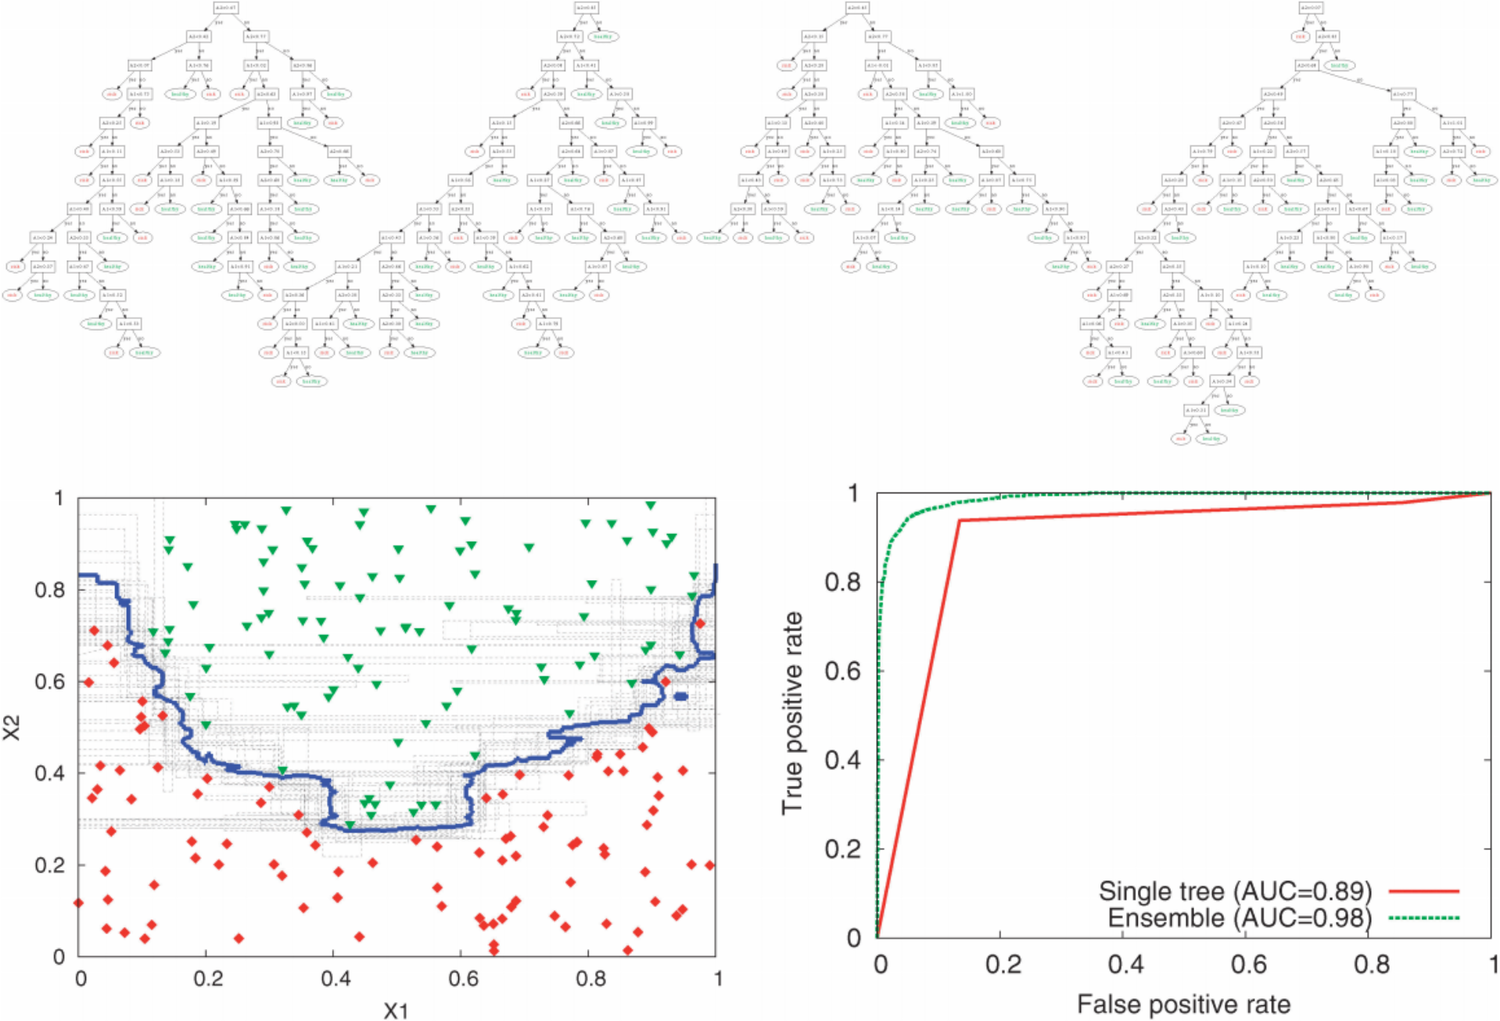
\includegraphics[width=1\columnwidth]{figures/regressiontrees/regressiontrees}
\caption{{Ensemble of decision trees (top) that produces a more accurate decision boundary (lower left) and comparison with a single tree model (lower right). Adapted with permission from \cite{Geurts_2009}.
\label{fig:tree_ensemble}%
}}
\end{center}
\end{figure}

Random forests use a form of cross-validation by training and testing each tree using a different bootstrapped sample from the data. This process produces an \emph{out-of-bag error (OOB)} that acts as a generalized error for understanding how well each class can be predicted. This accuracy is used to determine how well the generated temporal features can delineate the class objectives. Random forests can also calculate the importance of the input features and how well they lend themselves to predicting the objectives. This attribute is useful in that it allows us to understand exactly which temporal features are most characteristic of various objectives. Variable importance is calculated using Equation \ref{eq:varimportance}. The importance of input feature $X_m$ for predicting $Y$ by adding up the weighted impurity decreases $p(t)\Delta i(s_t,t)$ for all nodes $t$ where $X_m$ is used, averaged over all $N_T$ trees in the forest \cite{louppe2013understanding}.

\begin{equation}
Imp(X_m) = \frac{1}{N_T}\sum\limits_T\sum\limits_{t\in T:v(s_t)=X_m} p(t) \Delta i (s_t, t)
\label{eq:varimportance}
\end{equation}

\section{Case Study, Empirical Data Collection, and Qualitative Research}
\label{sec:screeningdata}

% One emerging trend is that "data mining algorithms should have as few parameters as possible, ideally none. A parameter-free algorithm prevents us from imposing our prejudices and presumptions on the problem at hand and let the data itself speak to us \citep{Keogh_2004}." This approach is known as \emph{parameter-free} or \emph{parameter-light} data mining. The efficacy of these algorithms has been proven comparable or better than many more complex, traditional time-series data mining approaches \citep{Keogh_2004}. This mantra is a primary objective of the feature extraction process outlined in this study.

One of the main goals of this research is the testing and implementation of the temporal feature extraction techniques on empirical sensor data collected from real buildings. Various raw data sets were obtained from case study buildings and campuses around the world to test the developed methods. The target of these interactions was to collect at least one year of hourly data from whole building electrical meters, resulting in at least 8760 measurements per building. Several of these data sets were collected through a series of site visits and interviews. These interactions are detailed in Section \ref{sec:sitevisit} by giving an in-depth overview of these case studies by discussing the current performance data acquisition systems and the standard methods of utilizing those data for tracking activities. A key goal of the collection of these data was that they would be a basis for an open, shareable data repository for building performance research. This goal was discussed with the case study participants. Several other raw data sets were collected from open data sources on the Internet and were included in this study, albeit often with less metadata available. These case studies are described in Section \ref{openonlinecasestudies}. 

In addition to the quantitative data collected from each of these case studies, qualitative feedback was gathered to get a better sense of \emph{how useful} the implementation and interpretation of the framework would be in the day-to-day operations of various types of stakeholders. The results of these qualitative interviews are included in this Section \ref{sec:characterization}.

\subsection{Site Visits for Case Studies}
\label{sec:sitevisit}
Throughout the course of two years, from February 2014 to April 2016, several site visits were conducted to interview operations staff at seven campuses. The purpose of this effort was two-fold: first, to collect as much raw, temporal data from each site as possible and, second, to discuss the status quo of building energy analysis as performed on their campus. This section discusses these site visits, the types of data that were collected, and a few of the lessons-learned from the process. A consistent theme in the site visits was that each campus has been investing in electrical metering and data acquisition systems over the past decade. In every one of the case study interviews, the operations staff discussed the underutilization of the data being collected. A common phrase was, "We have more meter data than any time before, and we don't know what to do with it." Another common situation was that a campus had a large electrical metering infrastructure but did not know how to extract raw data for this research project. This scenario occurred on three of the seven campuses after the first interview, and data was still not available even after a follow-up visit on two of those campuses. Therefore, only four of the seven case studies had data available and will be discussed in the following subsections.
%The methodology followed in this effort was drawn from mixed-method research techniques.

\subsubsection{Case Study 1} 
\label{sec:casestudy1}
The first case study is a campus in a continental climate in the Midwest region of the United States. It is a university with 226 buildings spread across two main campuses. Altogether, these buildings have a total floor area over 2.3 million square meters (25 million square feet). An initial interview was conducted with the lead statistician of the facilities management in March 2015. Information was gathered on the building and energy management systems of the campus and a discussion regarding the typical utilization of the data was conducted. It was found that there are over 480 electrical meters on the campus and that these data were primarily used for billing of the individual academic departments. They have a custom metering data management platform with some capabilities for data export. A second site visit was conducted in June 2015 to facilitate the collection of a sample one year data set. In this site visit, a facilities management professional with experience in SQL databases was able to directly query the underlying back-end of the energy management system to extract one year of raw data from all of the metering infrastructure on the campus. An accompanying meta-data spreadsheet was discovered that included information on floor area, primary space usage, EnergyStar score, and address. These data were then used for the analysis and feature extraction, and some of the results were compiled and presented to the entire facilities management department of this university in March 2016. This presentation gave an overview of the feature creation techniques and an understanding of how the buildings on their campus compare to other universities. More discussion on the feedback from this presentation are discussed in Section \ref{sec:characterization}.

\subsubsection{Case Study 2}
\label{casestudy2}
The second case study is a campus in the Northeast region of the United States. It is also a University and it has 180 buildings on a single main campus. An initial meeting was organized in April 2015 with the facilities management team. This campus has well-organized building and energy management systems with a strong emphasis on data acquisition and management. The campus has an analytics and automated fault detection software platform that is connected to the underlying controls systems. A follow-up campus visit was conducted in August 2015 to facilitate the download of a raw, example data set from the buildings on campus. At this point, a log-in to a new data management platform was given for the purposes data extraction. Several issues arose from the use of this platform and ultimately, a database query by the software developers of the system was used to extract the one year of electrical meter data from the campus buildings. Once again, a spreadsheet of meta-data was shared that included information on floor area and primary building use type. A final site visit was conducted in April 2016 to discuss some of the results of the data acquisition and upcoming plans for upgrades. A formal presentation of the results was not able to be given; thus only limited feedback of the implementation progress was collected.

\subsubsection{Case Study 3}
\label{sec:casestudy3}

The third case study is a campus in the Midwest region of the United States. Once again, it is a university campus with 25 buildings encompassing 204,000 square meters (2.2 million square feet) of floor space. An initial site survey and discussion of the campus was conducted in March 2015 with the campus lead mechanical and energy engineers. This campus has its electrical meters connected to a campus energy management platform that includes various visualizations and analytics techniques. This platform also can easily provide raw data download for analysis in this study. This platform resulted in this campus being by far the most user-friendly on data collection out of the case study set, including the open, on-line data sources. Raw data in flat files was easily downloaded for all data points at once. The meta-data for this campus was also extracted from this energy management platform, albeit in a more manual method from the user interface. A follow-up visit to this campus was conducted in March 2016 with initial results of characterizing the data according to a subset of the tested features. A significant amount of feedback for this case study was given by the facilities management department regarding the ability for these insights to assist in their decision-making processes. 

\subsubsection{Case Study 4}
\label{sec:casestudy4}

The fourth case study is an international school campus in tropical Southeast Asia. This campus includes five buildings with approximately 58,000 square meters (625,000 square feet). It was built and opened in 2010 and includes some sustainable design features such as an optimized chilled water plant, solar thermal cooling system, and an innovative, fresh air delivery system. The building management and data acquisition system have been a primary focus of the operations director of the campus for many years. Discussions and interviews with the operations staff have occurred numerous times over the course of the last five years. The key focus for this campus has been maintaining an optimized chilled water system. The operations team of this organization has been an active contributor to the development of the methodology. 

\subsubsection{Case Study 5}
\label{sec:casestudy5}

The final case study to be outlined in this section is a university campus located in Switzerland. This campus includes 22 building encompassing more than 150,000 square meters (1.6 million square feet). This campus has an energy management system with the ability to extract raw data, albeit only one point at a time. Data from this campus was utilized in a previous research project focused on campus and building-scale co-simulation and modeling. Only email correspondence with the campus facilities managers of this campus was conducted. A significant amount of meta-data was available from the facilities department through a spreadsheet that provided the breakdown of primary uses of the spaces in each building.

\subsection{Online Open Case Studies}
\label{openonlinecasestudies}

Several large data sets were found through a search of openly accessible data on-line. This section gives an overview of these data sources and the methods in which the data was extracted and pre-processed for analysis. Table \ref{tab:opendata} illustrates these sources, a short description of the platform in which the data was downloaded, and the URL of the platform. As in the site visit case studies, one year of hourly whole building electrical meter data was collected from each of these sources for as many buildings as possible.


\begin{table} 
\label{tab:opendata}
    \begin{tabular}{| p{4cm} | p{4cm} | p{6cm} |}
        \hline
        \textbf{Source Name} & \textbf{Description} & \textbf{Website}\\
        \hline
        Cornell University & EMCS Portal & http://portal.emcs.cornell.edu/ \\ 
        \hline
        University of California - Berkeley & Berkeley Campus Energy Portal & http://berkeley.openbms.org/\\ 
        \hline
        Arizone State University & Campus Metabolism & https://cm.asu.edu \\ 
        \hline
        Carbon Culture & Community Open Data Platform & https://platform.carbonculture.net \\ 
        \hline
        EnerNOC & EnerNOC GreenButton Data & https://open-enernoc-data.s3.amazonaws.com/anon/ index.html \\         
        \hline
        University of Southamption & Open Data Service & http://data.southampton.ac.uk/\\         
        \hline
    \end{tabular} 
    \caption{Open, online data sources} 
\end{table}


\section{Overview of Data Collected}
\label{sec:datacollected}

Through data collection from the on-site case study interviews and on-line data sources, whole building electrical meter data from 1238 buildings was collected. Figure \ref{fig:casestudymap} illustrates the locations of these building around the world. A majority of the buildings are located in the United States, with the highest concentrations in the northeast region. A wide range of building types are included in the data set, from Education and Government to Agriculture and Heavy Industry. 


\begin{figure}[ht!]
\begin{center}
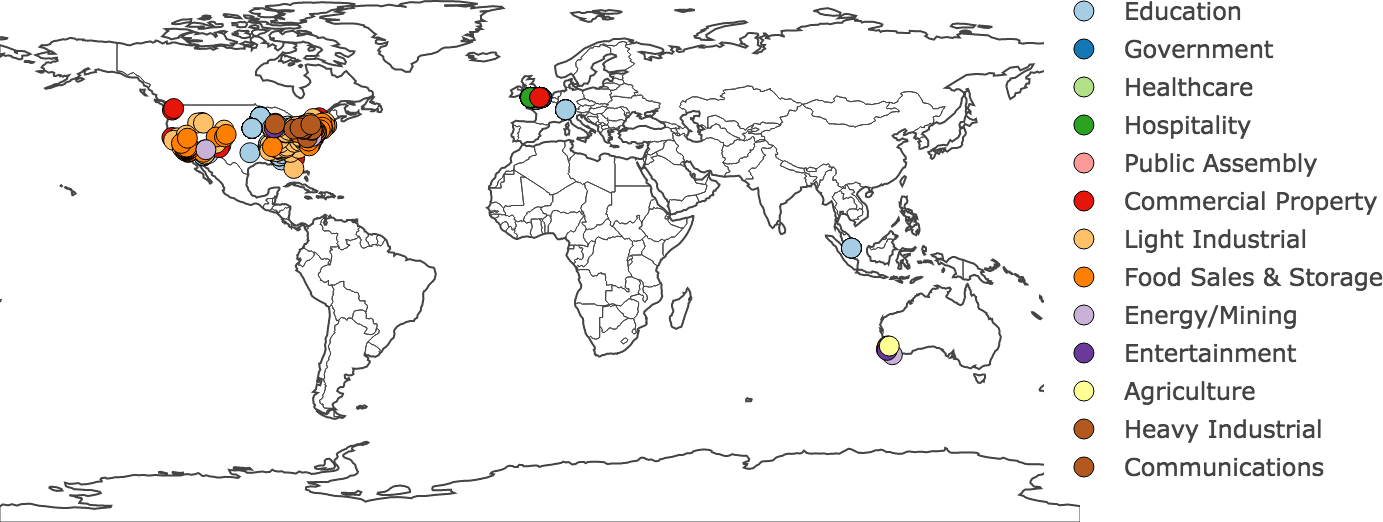
\includegraphics[width=0.98\columnwidth]{figures/casestudybuildinglocations/casestudybuildinglocations}
\caption{Locations of 1238 case study buildings collected from across the world
\label{fig:casestudymap}%
}
\end{center}
\end{figure}

From these groups of primary use types, the buildings are distributed across various time zone regions as seen in Figure \ref{fig:bar_primaryspaceuse}. The east coast of the United States is the largest group due to the number of campuses and buildings from the EnerNOC data source. All of the buildings from the Carbon Culture data source are located in the United Kingdom.

\begin{figure}[ht!]
\begin{center}
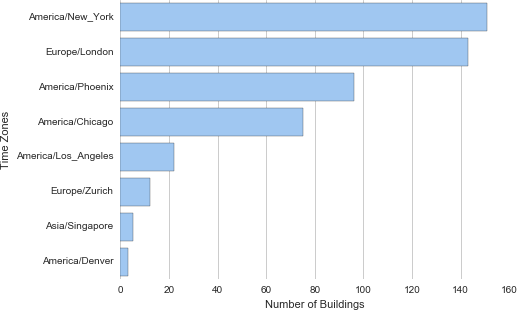
\includegraphics[width=0.98\columnwidth]{figures/timezonesbar1/timezonesbar}
\caption{Distribution of case study buildings amongst time zones
\label{fig:bar_timezone}%
}
\end{center}
\end{figure}

Figure \ref{fig:bar_industry} and \ref{fig:bar_subindustry} illustrate the industries and sub-industries that the case study buildings are collected from. The number of university campuses is strongly evident in both charts.

\begin{figure}[ht!]
\begin{center}
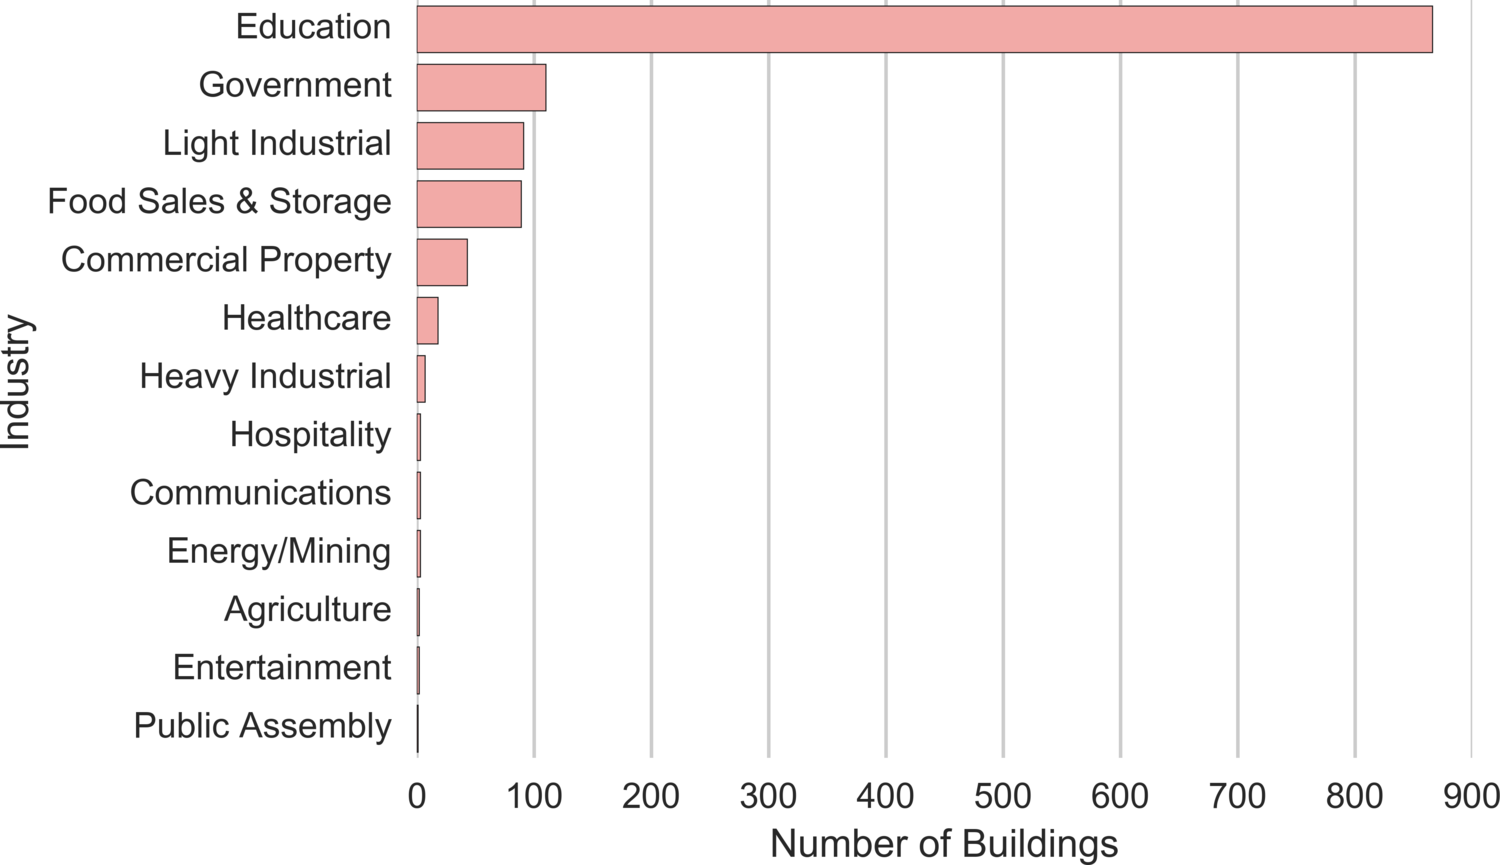
\includegraphics[width=0.98\columnwidth]{figures/bar_industry/bar_industry}
\caption{Distribution of case study buildings amongst general industries
\label{fig:bar_industry}%
}
\end{center}
\end{figure}

\begin{figure}[ht!]
\begin{center}
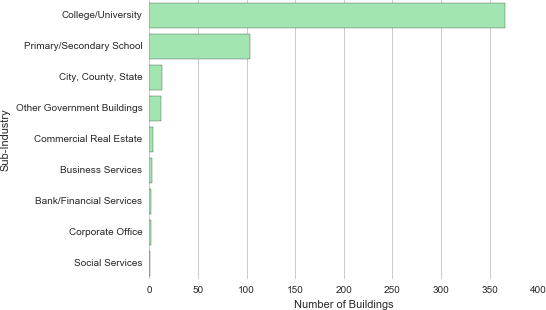
\includegraphics[width=0.98\columnwidth]{figures/bar_subindustry/bar_subindustry}
\caption{Distribution of case study buildings amongst sub-industries
\label{fig:bar_subindustry}%
}
\end{center}
\end{figure}

\subsection{Selection of Case Study Subset for Feature Implementation}
\label{casestudysubset}

A subset of buildings was chosen based on limiting criteria for inclusion in the implementation sections of this thesis. The primary consideration for inclusion is that the building is a member of one of the top primary use types: Offices, Primary/Secondary Schools, University Laboratories, University Classrooms, or Dormitories. These categories and the number of buildings in one are shown in Figure \ref{fig:bar_primaryspaceuse}.

\begin{figure}[ht!]
\begin{center}
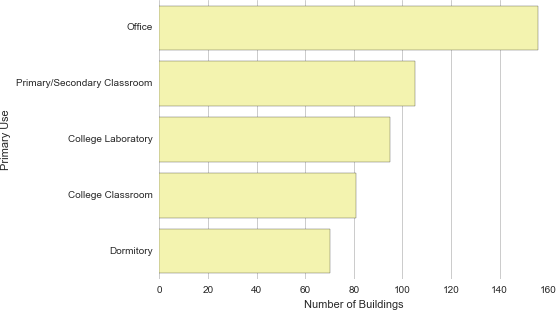
\includegraphics[width=0.98\columnwidth]{figures/bar_primaryspaceuse1/bar_primaryspaceuse}
\caption{Distribution of case study buildings amongst primary space uses
\label{fig:bar_primaryspaceuse}%
}
\end{center}
\end{figure}

\section{Advanced Metering Infrastructure Case Study}
\label{sec:smartmeterdata}

A larger data set of almost 10,000 non-residential buildings is gathered in this thesis from an organization tasked with using the data to target buildings for performance improvement measures. These data are from an Advanced Metering Infrastructure (AMI) implementation. Different types of meta-data are available for these buildings, including industry and energy savings measure implementation. The primary goal of this data set is to provide a context of scalability on a larger data set. These data are strictly private and detailed data cannot be included in the methodology or development of the framework.


\chapter{Statistics-based Features}
\label{sec:statisticsfeatures}

Statistics-based temporal features are the first and most simplified category of temporal features developed. The main classes of features are basic temporal statistics, ratio-based, and the Spearman rank order correlation coefficient.

\section{Theoretical Basis}
\subsection{Basic Temporal Statistics}
\label{sec:basicstatistics}

The first set of temporal features to be extracted are basic statistics-based metrics that utilize the time-series data vector for various time ranges to obtain information using mean, median, maximum, minimum, range, variance, and standard deviation. Many of these features are developed through the implementation of the VISDOM package in the R programming language \citep{visdom_borgeson}.As a simple example, if a time-series vector is described as $X$, with $N$ values of $X = {x_1, x_2,...,x_n}$, the most common statistical metric, mean (or $\mu$), can be calculated using Equation \ref{eq:mean} \citep{Mitsa_2010}.

\begin{equation}
\mu = \frac{\sum\limits_{i=1}^N x_i}{N}
\label{eq:mean}
\end{equation}

The mean is taken not just for the entire time series, but also from the summer and winter seasons. The variance of the values are taken for the whole year, the summer and winter seasons as well. The variance of daily mean, minimum, and maximum values are determined to understand the breadth of values across the time range. Variance is calculated according to Equation \ref{eq:variance}. 


\begin{equation}
\sigma^2 = \frac{\displaystyle\sum_{i=1}^{n}(x_i - \mu)^2} {n}
\label{eq:variance}
\end{equation}

The maximum and minimum electrical demand are calculated. Additionally, the hour and date at which the maximum demand occurs are determined to understand when peak consumption occurs. Additionally, the temperature at the maximum and minimum is account for weather influence. The 97th and 3rd percentiles are calculated to exclude any extreme outliers, a value that's often more useful than the maximum and minimum.\\ 

A series of hour-of-day (HOD) metrics are calculated that relate to aggregating the behavior occurring at each of hour the day-four metrics. The first of these calculates the most current hour of the top demand of the top 10\% hottest days and the most common hour of the top 10\% temperatures to inform roughly about cooling energy consumption. These metrics are repeated from the bottom 10\% coldest days and temperatures. Another set of twenty-four metrics is calculated to account simply for the mean demand of each hour of the day.\\

A set of metrics is calculated individually for January and August to account for potential heating and cooling seasons. The daily maximum, minimum, mean, range and load duration are calculated for these seasonal periods. The complete list of these features can be found in Appendix \ref{sec:temporalfeaturelist}.


\subsection{Ratio-based Statistical Features}
\label{sec:ratiobasedfeatures}

%to get a sense of what a temporal feature is in the context of electrical meters for buildings, t

The second major category of statistical features is ratio-based features. Simply, these are metrics in which two or more of the previously calculated statistical metrics are combined as a ratio. These features often have a \emph{normalizing effect} in which buildings can be more appropriately compared to each other. The first extracted metric of this type is one of the most commonly calculated for building performance analysis: the consumption magnitude of electricity normalized by the floor area of the building. This metric seeks to provide a basis for comparison between buildings and is used as a key metric within numerous benchmarking and performance analysis techniques. Figure \ref{fig:normalizedmag} illustrates a single building example of this metric per hour across a time range of two weeks at the end of the year. The top line chart of this figure shows the magnitude of hourly electrical consumption for one of the case study buildings. The middle portion of the figure repeats this information in the form of a color-based, one-dimensional heatmap. In this example, the daily weekday profiles manifest themselves as light-colored bands and weekend and unoccupied periods as darker bands. The color bar at the bottom of the figure is key in interpreting the color values. This figure is an example of a single building demonstration of this particular feature and is a type of graphic that is used throughout this entire section.

\begin{figure}[ht!]
\begin{center}
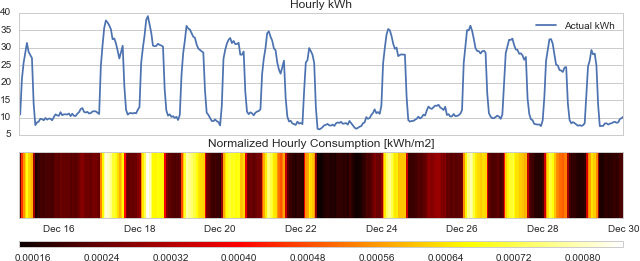
\includegraphics[width=1\columnwidth]{figures/normalizedcons_example/normalizedcons_example}
\caption{Single building example of area normalized magnitude
\label{fig:normalizedmag}%
}
\end{center}
\end{figure}

After normalized consumption, the first set of temporal features to be extracted are primary statistics-based metrics that utilize the time-series data vector for various time ranges to retrieve information using mean, median, maximum, minimum, range, variance, and standard deviation. If a time-series vector is described as $X$, with $N$ values of $X = {x_1, x_2,...,x_n}$, the most common statistical metric, mean (or $\mu$), can be calculated using Equation \ref{eq:mean} \citep{Mitsa_2010}.

\begin{equation}
\mu = \frac{\sum\limits_{i=1}^N x_i}{N}
\label{eq:mean}
\end{equation}

The median value of a vector is simply the middle value in an ordered set if the number of values is odd. If the length of the vector is even, then the median is the mean of the two middle values. The minimum and maximum values are the first and last in an ordered set. Vectors of values can also be described according to percentiles. Percentiles are cutpoints dividing the range of a probability distribution based on the percentage of values below a given threshold. For example, the value at the 95\% percentile is found 95\% of the way along an ordered set, with only 5\% of the values remaining before reaching the maximum. In this section, aggregation ratios of many of these collection techniques are applied to the 24 hours from a single day to characterize various types of typical behavior quickly. The first example of these ratios is the minimum versus maximum ratio or load ratio. This rate is calculated by taking the daily minimum and dividing it by the daily maximum. Figure \ref{fig:loadratio_singlebuilding} illustrates a single building example of this ratio on one month of data from a case study building. These load ratios indicated whether a daily profile is more diverse, resulting in a lower load ratio, or more flat, resulting in a higher load ratio. In this example, weekends and holidays are a darker shade of blue as compared to generally-occupied weekdays. Load ratio can be used an indicator also of the relative magnitude of the unoccupied baseline. Buildings that have a lower average load ratio often have higher than average baselines, such as in laboratories or hospitals.

\begin{figure}[ht!]
\begin{center}
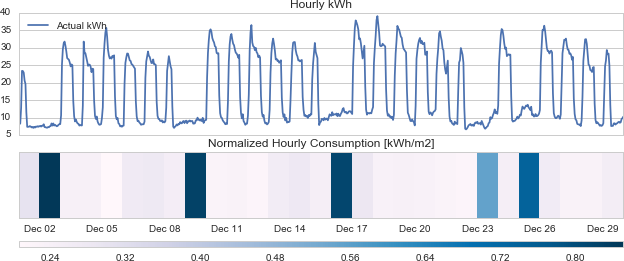
\includegraphics[width=1\columnwidth]{figures/loadratio_example/loadratio_example}
\caption{Single building example of the daily load ratio statistic
\label{fig:loadratio_singlebuilding}%
}
\end{center}
\end{figure}

% Daily load ratio is another simplified example of characterizing the minimum vs. maximum for each day.

% One of the primary functions of the built environment is to provide a thermally comfortable environment for occupants. These systems utilize electricity for the primary or secondary heating, ventilation, and air-conditioning systems (HVAC). Various metrics are developed in this effort to quantify the impact outdoor air conditions have on electricity performance.

A library of similar load ratio daily metrics is designed and implemented on the case study buildings. These other ratios are daily mean versus maximum, minimum versus 95\% percentile, and mean versus 95\% percentile. The use of the 95\% metric is mean to mitigate against outliers skewing the load ratios. These ratios are calculated on all days in the set, as well as just for weekend and weekdays. A full list of the features generated is found in Appendix A.

\subsection{Spearman Rank Order Correlation Coefficient}
\label{sec:weathercorrelationcoeff}

Data stream influence characterization is the process of roughly classifying the dataset into streams and subsequences based on weather conditions sensitivity. A feature is developed in a study of evaluation of campus data for simulation feedback, and the following is a summarization of this technique \citep{miller_forensically_2015}. This evaluation is important in understanding what measured performance is due to heating, cooling, and ventilation systems (HVAC) responses to outdoor conditions and what is due to schedule, occupancy, lighting, and different loading conditions which are weather independent. Performance data that is influenced by weather can be used to understand the HVAC system operation better or be weather-normalized to understand occupant diversity schedules. %Non-weather sensitive data streams are used with less pre-processing to create diversity schedules and to calculate miscellaneous and lighting load power densities. T

The Spearman Rank Order Correlation (ROC) is used to evaluate the positive or negative correlation between each performance measurement stream and the outdoor air dry bulb temperature. This technique has been previously used for weather sensitivity analysis \citep{coughlin_statistical_2009}. The ROC coefficient, $\rho$, is calculated according to a comparison of two data streams, $X$, and $Y$, in which the values at each time step, $X_i$, and $Y_i$, are converted to a relative rank of magnitude, $x_i$ and $y_i$, according to its respective dataset. These rankings are then used to calculate $\rho$ that varies between +1 and -1 with each extreme corresponding to a perfect positive and negative correlation respectively. A value of 0 signifies no relationship between the datasets. This $\rho$ value for a time-series is calculated according to Equation \ref{eq:spearman}.

\begin{equation}
\rho = 1 - \frac{6\sum d_i^2}{n(n^2-1)}
\label{eq:spearman}
\end{equation}

The difference between the data stream rankings, $x_i$ and $y_i$, is signified by a difference value, $d_i$, and the number of samples compared to each dataset is signified by $n$. Figure \ref{fig:weather_examples_plot} illustrates the calculation of the ROC coefficient, $\rho$ for three examples. The cooling sensitive data set shows a strong positive correlation between outside air temperature and energy consumption with a $\rho$ value of 0.934. As the outside air temperature increases, the power consumption measured by this meter increases. The heating sensitive dataset shown has a strong negative correlation with a $\rho$ of -0.68. A weather-insensitive dataset is shown in the middle which has a $\rho$ of 0.0, signifying no weather relationship, which is evident due to the four levels of consumption which are independent of outdoor air conditions.

\begin{figure}[ht!]
\begin{center}
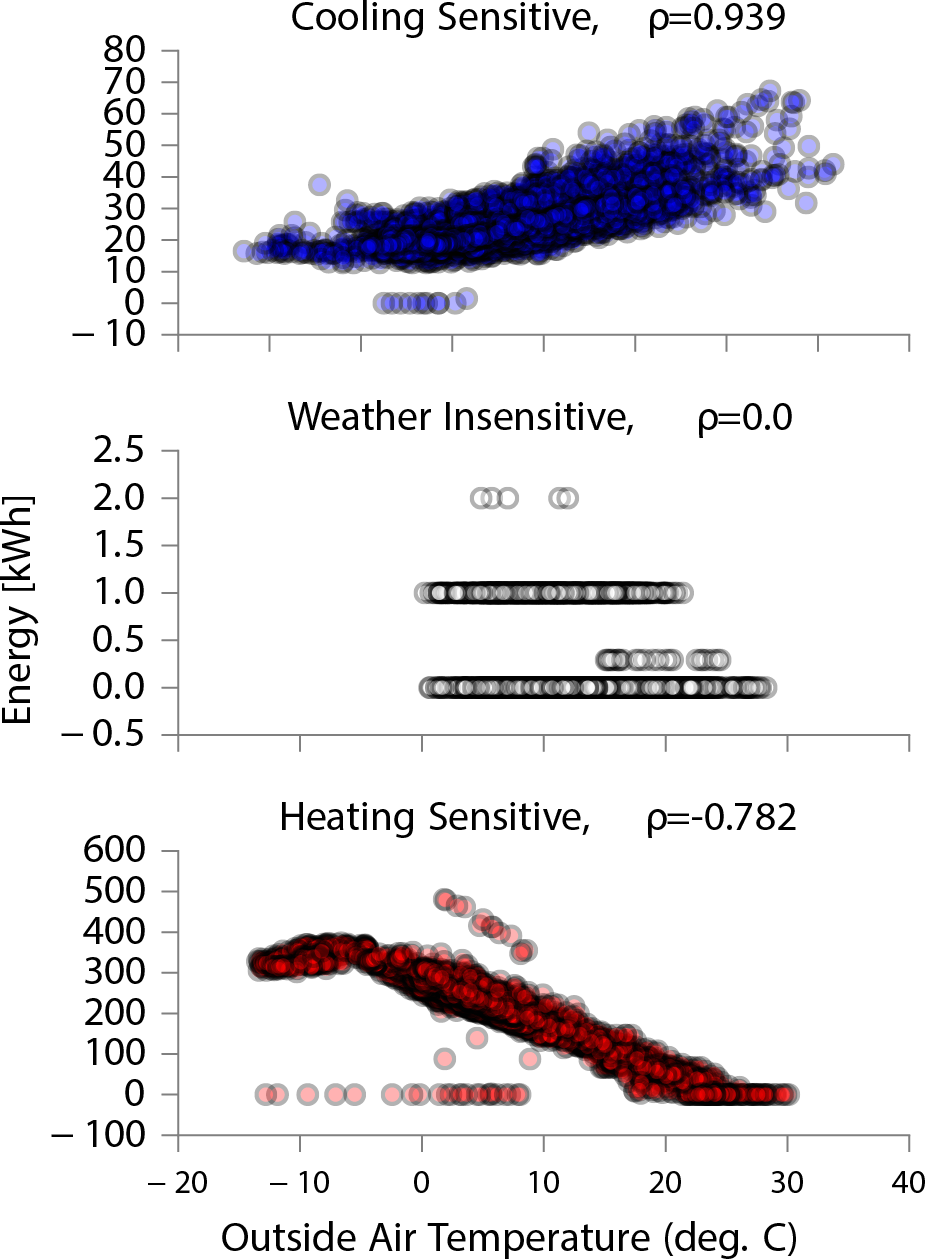
\includegraphics[width=0.5599999999999999\columnwidth]{figures/weathersensitivity/weathersensitivity}
\caption{Weather sensitivity examples as energy vs. outdoor air temperature (from \citep{miller_forensically_2015})
\label{fig:weather_examples_plot}%
}
\end{center}
\end{figure}

The correlation coefficient can be visualized for a single case as seen in Figure \ref{fig:spearman_singlebuilding}. The coefficient, in this case, is calculated individually for each month. This process results in twelve calculations of the metric using between 29-31 samples. In this case, consumption in January to May is noticeably more heating sensitive, a fact that can be observed clearly from the line chart, as well as the one dimension heat map. May to November is more cooling sensitive. It is interesting that September appears to be the most cooling sensitive month, a fact perhaps related to use schedules during that month. This coefficient is not a perfect indicator of HVAC consumption; it just detects a correlation. However, it is fast and easy to calculate and is the first phase of detecting weather dependency. More detailed and informative weather influence extraction features are investigated in Section \ref{sec:regressionmodels}.

\begin{figure}[ht!]
\begin{center}
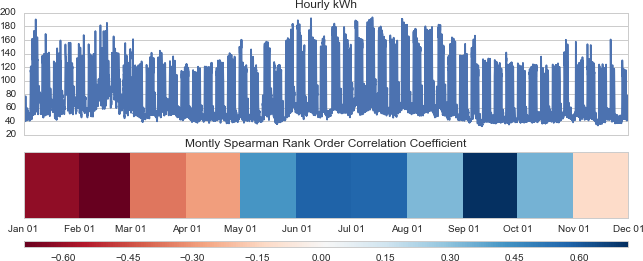
\includegraphics[width=1\columnwidth]{figures/spearman_example/spearman_example}
\caption{Single building example of the spearman rank order correlation coefficent with weather
\label{fig:spearman_singlebuilding}%
}
\end{center}
\end{figure}

\section{Implementation and Discussion}
Figure \ref{fig:normalizedcons_heatmap} illustrates the same normalized consumption metric as applied to all of the case study buildings. There are five segments of buildings based on the primary use types within the set: offices, university laboratories, university classrooms, primary/secondary schools, and university dormitories. These metrics are visualized in this way to understand the difference between each of these use types for each of the presented metrics. Each row of the heatmap for each segment is the values of the feature for a single building, while the x-axis is the time range for all buildings. Not all of the case study buildings have a January to December time range. For these cases, the data was rearranged so that a continuous set of January to December data is available to be visualized in the heat map. The aggregation metrics themselves are not calculated with this rearranged vector; it is only for visualization purposes. Like Figure \ref{fig:normalizedmag}, this type of graphic is used to visualize many of the temporal features in this section. From this metric in particular, one will notice that university labs have a systematically higher consumption over time as compared to the other use types. One will also see the dark vertical lines across the time range indicating weekend use as compared to the weekday. This particular pattern is absent from university dormitories due to their more continuous energy consumption.

\begin{figure}[ht!]
\begin{center}
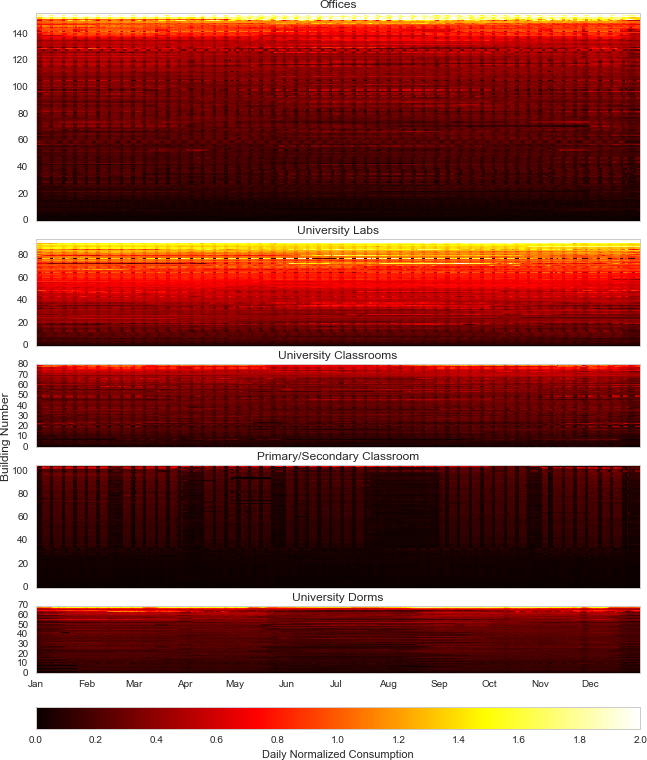
\includegraphics[width=1\columnwidth]{figures/normalizedcons_heatmap/normalizedcons_heatmap}
\caption{Heat map representation of normalized magnitude
\label{fig:normalizedcons_heatmap}%
}
\end{center}
\end{figure}

Figure \ref{fig:loadratio_heatmap} illustrates this metric as applied to all case study buildings. As in the normalized magnitude, various patterns are more apparent including the weekday versus weekend phenomenon.

\begin{figure}[ht!]
\begin{center}
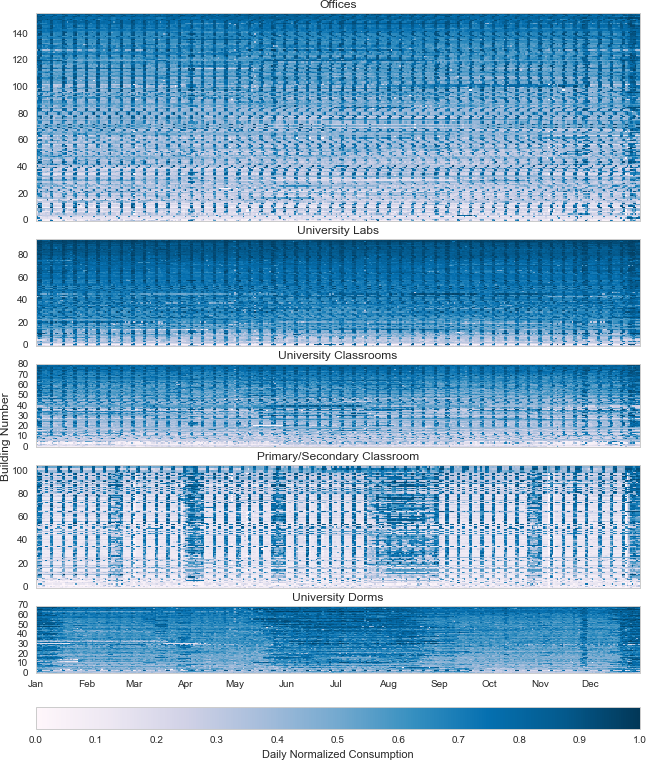
\includegraphics[width=1\columnwidth]{figures/loadratio_heatmap/loadratio_heatmap}
\caption{Heatmap of daily load ratio statistic for all case study buildings
\label{fig:loadratio_heatmap}%
}
\end{center}
\end{figure}

\begin{figure}[ht!]
\begin{center}
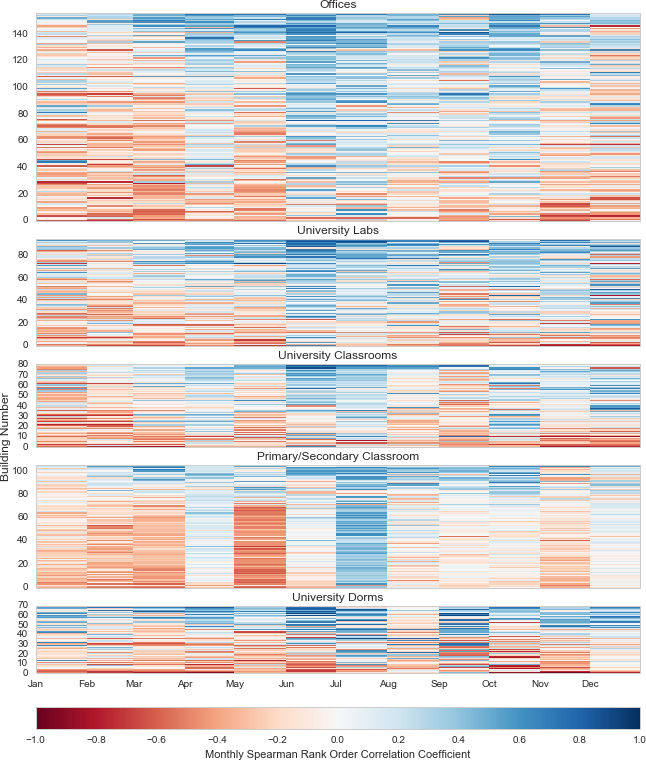
\includegraphics[width=1\columnwidth]{figures/spearman_heatmap/spearman_heatmap}
\caption{Heatmap of spearman rank order correlation coefficient for all case study buildings
\label{fig:spearman_heatmap}%
}
\end{center}
\end{figure}


\chapter{Regression Model-based Features}
\label{sec:regressionmodels}

Semi-physical behavior about a building can be extracted by using performance prediction models and using output parameters and goodness-of-fit metrics for characterization. This section covers the use of several common electrical consumption prediction models to create sets of temporal features useful for characterization of buildings. Section \ref{sec:modelbasedtheory} covers the theory underlying each technique and Section \ref{sec:modelbaseddiscussion} discusses the implementation of the case study data with a focus on underlying trends as related to building use type.

\section{Theoretical Basis}
\label{sec:modelbasedtheory}
\subsection{Load shape regression-based Features}
\label{sec:regressionmetrics}

Prediction of electrical loads based on their shape and trends over time is a mature field developed to forecast consumption to detect anomalies and analyze the impact of demand response and efficiency measures. The most common technique in this category is the use of heating and cooling degree days to normalize monthly consumption \citep{fels_prism:_1986}. Over the years, various other techniques have been developed using techniques such as neural networks, ARIMA models, and more complex regression \citep{taylor_comparison_2006}. However, simplified methods have retained their usefulness over time due to ease of implementation and accuracy. In the context of temporal feature creation, a regression model provides various metrics that describe how well a meter conforms to conventional assumptions. For example, if actual measurements and predicted consumption match well, the underlying behavior of energy-consuming systems in the building has been captured adequately. If not, there is the uncharacterized phenomenon that will need to be obtained with a different type of model or feature. 

A contemporary, simplified load prediction technique is selected to create temporal features that capture whether the electrical measurement is simply a function of time-of-week scheduling. This model was developed by Matthieu et al. and Price and implemented mostly in the context of electrical demand response evaluation \citep{price_methods_2010, mathieu_quantifying_2011}. The premise of the model is based on two features: a time-of-week indicator and an outdoor air temperature dependence. This model is also known as the \emph{Time-of-week and Temperature or (TOWT)} model or \emph{LBNL regression model} and is implemented in the \emph{eetd-loadshape} library developed by Lawrence Berkeley National Laboratory\footnote{https://bitbucket.org/berkeleylab/eetd-loadshape}.

According to the literature, the model operates as follows \citep{price_methods_2010}. The time of week indicator is created by dividing each week into a set of intervals corresponding to each hour of the week. For example, the first interval is Sunday at 01:00, the second is Sunday at 02:00, and so on. The last, or 168th, interval is Saturday at 23:00. A different regression coefficient, $\alpha_i$, is calculated for each interval in addition to temperature dependence. The model uses outdoor air temperature dependence to divide the intervals into two categories: one for occupied hours and one for unoccupied. These modes are not necessarily indicators of exactly when people are inhabiting the building, but simply an empirical indication of when occupancy-related systems are detected to be operating. Separate piecewise-continuous temperature dependencies are then calculated for each type of mode. The outdoor air temperature is divided into six equally sized temperature intervals. A temperature parameter, $\beta_j$, with $j = 1...6$, is assigned to each interval. Within the model, the outdoor air temperature at time, $t$, occurring at time-of-week, $i$, (designated as $T(t_i)$) is divided into six component temperatures, $T_{c,j}(t_i)$. Each of these temperatures is multiplied by $\beta_j$ and then summed to determine the temperature-dependent load. For occupied periods the building load, $L_o$, is calculated by Equation \ref{eq:tempdepload}.

\begin{equation}
\label{eq:tempdepload}
L_0(t_i,T(t_i) = \alpha_i + \sum_{j=1}^{6}\beta_j T_{c,j}(t_i)
\end{equation}

Prediction of unoccupied mode occurs using a single temperature parameter, $\beta_u$. Unnoccupied load, $L_u$, is calculated with Equation \ref{eq:nontempdepload}.

\begin{equation}
\label{eq:nontempdepload}
L_0(t_i,T(t_i) = \alpha_i + \beta_u T_{c,j}(t_i)
\end{equation}

The primary means of temporal feature creation from this process is through the analysis of model fit. The first metric calculated is a normalized, hourly residual, $R$, that can be used to visualize deviations from the model. It is calculated from the actual load, $L_a$, and the predicted load, $L_p$. The residual at a specific hour, $t$, is calculated using Equation \ref{eq:residualerror}.

\begin{equation}
\label{eq:residualerror}
R_t = \frac{L_{t,a} - L_{t,p}}{max_{L_a}}
\end{equation}

An example of the TOWT model implemented on one of the case study buildings is seen in Figure \ref{fig:loadshape_single}. Two primary characteristics are captured from a model residual analysis. The first is the building's primary deviation from a set time-of-week schedule and behavior causing the model to highly over-predict. These deviations are most often attributed to public holidays, breaks in normal operation, or changes in normal operating modes. In the single building study, one of the most obvious daily deviations, Christmas Day, is observed. This day is significantly over-predicted due to the model not being informed of the Christmas Day holiday. The automated capture of this phenomenon can inform whether the building is of a certain use-type or in a certain jurisdiction. The second characteristic captured are periods of under prediction when the building is consuming more electricity than expected. These data inform whether a building is being consistently utilized, or whether there is volatility in its normal operating schedule from week-to-week. 

\begin{figure}[ht!]
\begin{center}
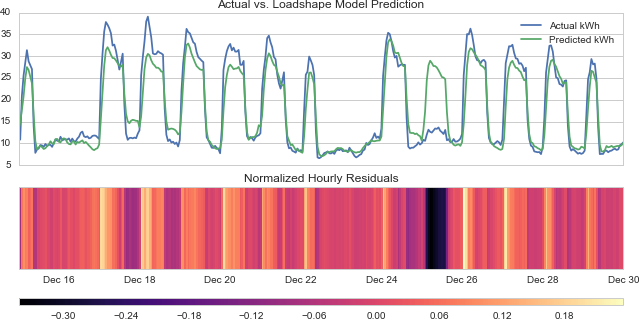
\includegraphics[width=1\columnwidth]{figures/loadshape_example/loadshape_example}
\caption{Single building example of TWOT model with hourly normalized residuals
\label{fig:loadshape_single}%
}
\end{center}
\end{figure}

\subsection{Change Point Model Regression}
\label{sec:changepointmodels}

Another means of performance modeling that takes weather characterization into consideration is the use of linear change point models. The outputs of these models can be interpretable in approximating the amount of energy being used for heating, ventilation, and air-conditioning (HvAC). This type of model has its basis in the previously-mentioned PRISM method and has been continuously utilized, recently by Kissock and Eger \citep{Kelly_Kissock_2008}. This multivariate, piece-wise regression model is developed using daily consumption and outdoor air dry-bulb temperature information. A linear regression model is fitted to data detected to be correlated with outdoor dry-bulb air temperature, either positively for cooling energy consumption or negatively for heating energy consumption. For example, as the outdoor air temperature climbs above a certain point, the relationship between electrical consumption and every degree increase in temperature should be a linear line with a certain slope if the building has an electrically-driven cooling system. The point at which this change occurs is considered the cooling balance point of the building and the slope of the line is the rate of cooling energy increase due to outdoor air conditions. This example can be seen in Figure \ref{fig:changepointmodels}a in which the base load of the building is designated as $\beta_1$, the slope of the cooling energy line is $\beta_2$, and the change point temperature is $\beta_3$. Heating energy, as seen in Figure \ref{fig:changepointmodels}b, is similar except that the slope of the line will be negative; as temperature decreases, the heating energy increases. An optimization algorithm is used to detect each of these parameters from either hourly or daily raw data.

\begin{figure}[ht!]
\begin{center}
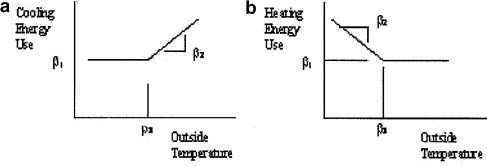
\includegraphics[width=0.84\columnwidth]{figures/changepointmodel_kissock/changepointmodel_kissock}
\caption{Example of an (a) 3 point cooling and (b) 3 point heating change point models (Used with permission from \citep{kelly_kissock_measuring_2008})
\label{fig:changepointmodels}%
}
\end{center}
\end{figure}

Equations \ref{eq:coolingenergy} and \ref{eq:heatingenergy} are used to predict energy energy consumption based on an outdoor air temperature, $T$. This equation can also predict the heating ($\beta_2(T - \beta_3)$) or cooling ($\beta_2(\beta_3 - T)$) components of the electrical consumption to a certain level of accuracy. 

\begin{equation}
\label{eq:coolingenergy}
E_c = \beta_1 + \beta_2(T - \beta_3)
\end{equation}

\begin{equation}
\label{eq:heatingenergy}
E_h = \beta_1 + \beta_2(\beta_3 - T)
\end{equation}

Figure \ref{fig:changepoint} illustrates a change point model fit on an office building in a continental climate that includes both heating and cooling seasons. It should be noted that the model is not perfectly characterizing the data due to two modes of daily operation; this situation is due to there being an offset between occupied and unoccupied operation. This model is used to generate features of approximate heating and cooling energy and in general, the slopes of these two modes can safely be assumed to be similar in most cases. The Open Meter Python library is used to regress these models for each building in this study \footnote{http://www.openeemeter.org/}.

\begin{figure}[ht!]
\begin{center}
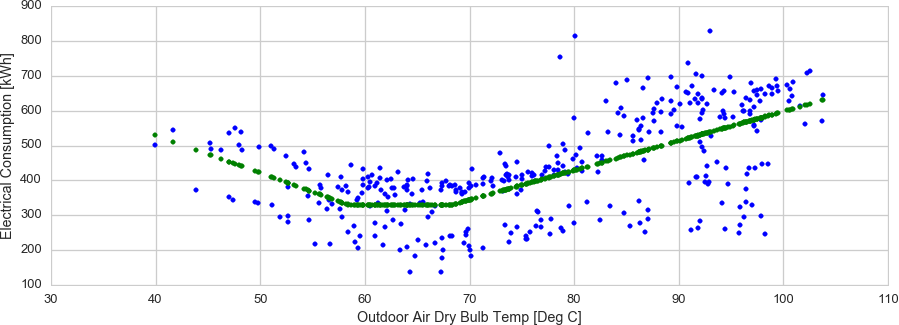
\includegraphics[width=1\columnwidth]{figures/Changepointmodelexample/Changepointmodelexample}
\caption{Single building example of change point model of a building
\label{fig:changepoint}%
}
\end{center}
\end{figure}

Figures \ref{fig:cooling_single} and \ref{fig:heating_single} illustrate single building examples of using the regression model to extract the approximate heating and cooling electrical consumption from the overall power meter. The cooling consumption example illustrates cooling consumption primarily in the summer-time season, as expected. An interesting aspect of this example is that there are a couple days of predicted cooling consumption in November and December. These days are due to outdoor air temperature crossing the balance point in anomalous ways during that season. The heating consumption example also resembles an intuitive understanding how the heating season from December to mid-April. In each example, one notices a correlation between the cooling and heating consumption in the heat-map and slight increases in the line charts indicating seasonality. 

\begin{figure}[ht!]
\begin{center}
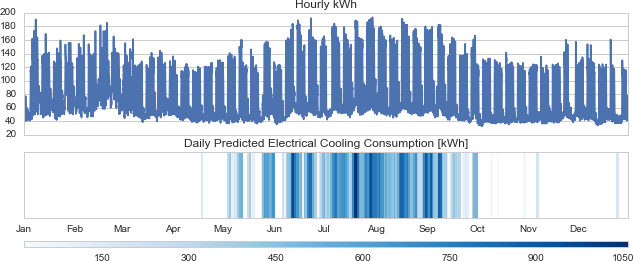
\includegraphics[width=1\columnwidth]{figures/cooling_example/cooling_example}
\caption{Single building example of predicted electrical cooling energy using change point model
\label{fig:cooling_single}%
}
\end{center}
\end{figure}

\begin{figure}[ht!]
\begin{center}
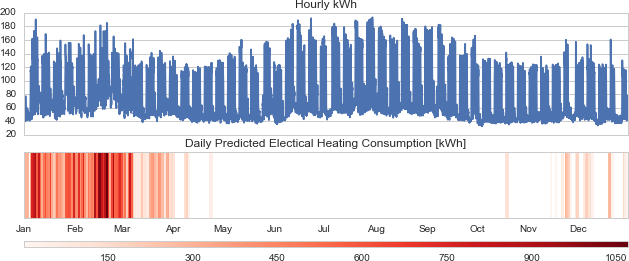
\includegraphics[width=1\columnwidth]{figures/heating_example/heating_example}
\caption{Single building example of predicted electrical heating energy using change point model
\label{fig:heating_single}%
}
\end{center}
\end{figure}

\subsection{Seasonality and Trend Decomposition}
\label{sec:seasonaldecomposition}

Temporal, or time series data, from different sources, often exhibit similar types of behavior that are studied within the field of forecasting and temporal data mining. Electrical building meter data fits within this category, and the same feature extraction techniques can be applied as what is commonly done for financial or social science analysis. These techniques often seek to decompose time-series data into several components that represent the underlying nature of the data \citep{Mitsa_2010}. For example, the electrical meter data collected from buildings is often cyclical in its weekly schedule. People are utilizing buildings each day of the week in a relatively predictable pattern. A very common example of this behavior is found in office buildings where occupants are typical white collar professionals who come into work on weekdays at a particular time and leave to go home at a certain time. Weekends are unoccupied periods in which there is little to no activity. This behavior is an example of what's known as seasonality within time series analysis. Seasonality is a fixed and known period of consistent modulation and is a feature that is often extracted before creating predictive models. 

Trends are another feature commonly found in temporal data. A trend is a long-term increase or decrease in the data that often doesn't follow a particular pattern. Trends are commonly due to factors that are less systematic than seasonality and are often due to external influences. For building energy consumption, trends manifest themselves as gradual shifts in consumption over the course of week or months. Often these shifts are due to weather-related factors having an influence on the HVAC equipment. Other causes of trends are changes in occupancy of degradation of system efficiency. 

To capture these features to understand their impact on characterizing buildings, the seasonal-trend decomposition procedure based on loess is used to extract each of these features from the case study buildings \citep{cleveland1990stl}. This process is used to remove the weekly \emph{seasonal} patterns from each building, the long-term trend over time, and the residual remainders from the model developed by those two components. The input data is aggregated to daily summations and weather normalized by subtracting the calculated heating and cooling elements from the change point model described in Section \ref{sec:changepointmodels}. This step is done to reduce the influence weather plays in the trend decomposition. The \emph{STL} package in R is used for this process to extract the seasonal, trend, and irregular components \footnote{https://stat.ethz.ch/R-manual/R-devel/library/stats/html/stl.html}. 

The details of the inner algorithms of the \emph{STL} procedure are described by Cleveland et al. \citep{cleveland1990stl}. The process uses an inner loop of algorithms to detrend and deseasonalize the data by creating a trend component, $T_v$, and a seasonal component, $S_v$. The remainder component, $R_v$, is a subtraction of the input values, $Y_v$ as seen in Equation \ref{eq:stl_residualscalc}.

\begin{equation}
\label{eq:stl_residualscalc}
R_v = Y_v - T_v - S_v
\end{equation}

 An output of the process of the \emph{STL} package is seen in Figure \ref{fig:stl_decomposition}. The \emph{data} component is the weather-normalized electrical meter data, the \emph{seasonal} component is decomposed weekly pattern, the \emph{trend} is the smoothed trend component, and the \emph{remainder} is the residual after the other components have been subtracted out.


\begin{figure}[ht!]
\begin{center}
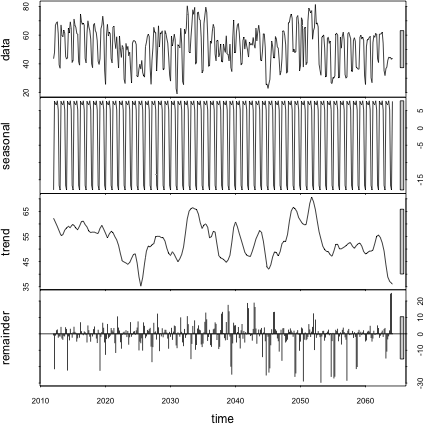
\includegraphics[width=0.7\columnwidth]{figures/stl_explanation/stl_explanation}
\caption{Output of seasonal decomposition process using loess for a single building.
\label{fig:stl_decomposition}%
}
\end{center}
\end{figure}

The seasonal component of this decomposition process can then be extracted to get an understanding of the typical weekly pattern of a building's electrical consumption. Figure \ref{fig:weeklypattern_single} illustrates this situation for a single building that has a typical office-style utilization schedule with a Monday to Friday working schedule with Saturday and Sunday off. This metric has been normalized to make it comparable to other buildings.

\begin{figure}[ht!]
\begin{center}
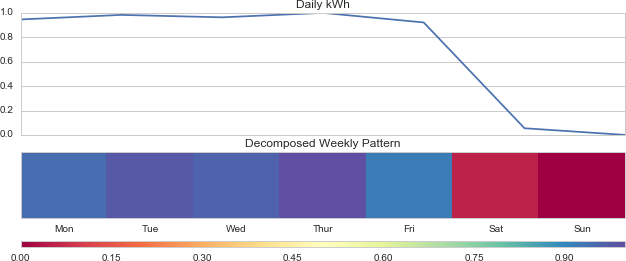
\includegraphics[width=1\columnwidth]{figures/stl_seasonal_example/stl_seasonal_example}
\caption{Single building example of decomposed weekly patterns using the \emph{STL} process
\label{fig:weeklypattern_single}%
}
\end{center}
\end{figure}


The general trend over the course of the year of data is another example of quantifying the seasonal patterns in utilization of a building. Weather influence has been reduced or removed using the change point models. Therefore, a trend could be the result of changes in building occupancy due to breaks, changes in equipment or space functions that would significantly increase or decrease the consumption, or gradual faults in systems of equipment. Figure \ref{fig:trend_single} illustrates a single building example of a decomposed trend for a building. January to May is in the middle range of consumption trend with a noticeable dip in April. From June to Oct, there is a trend upwards of higher than normal consumption, perhaps due to higher utilization of the space. October to the end of the year is back to average with a slight dip during the last few weeks of the year.

\begin{figure}[ht!]
\begin{center}
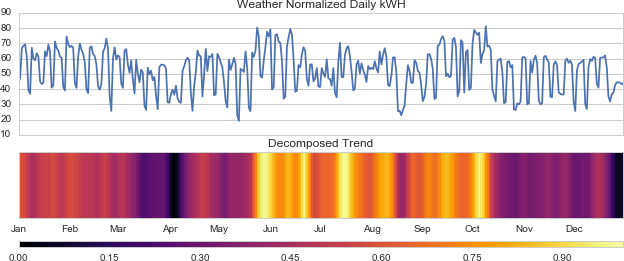
\includegraphics[width=1\columnwidth]{figures/stl_weathernorm_trend_example/stl_weathernorm_trend_example}
\caption{Single building example of decomposed trend using the \emph{STL} process
\label{fig:trend_single}%
}
\end{center}
\end{figure}


The remainder values of the \emph{STL} decomposition process are indicators of days that fall outside of the \emph{STL} model's prediction. This situation is similar to the residuals of the \emph{loadshape} models in Section \ref{sec:regressionmetrics}. Figure \ref{fig:remainder_single} illustrates an example of the residual days. Once again, this metric is normalized, however not on a 0 to 1 range. Instead, negative values indicate a lower than expected consumption for the day, while positive values are higher than average. In this example, the residuals aren't exceptionally systematic. However, a few identifiable days can be seen including Thanksgiving in November.

\begin{figure}[ht!]
\begin{center}
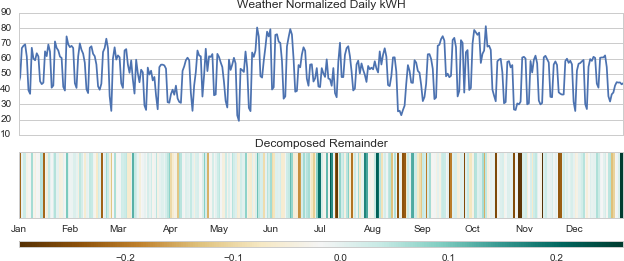
\includegraphics[width=1\columnwidth]{figures/stl_weathernorm_remainder_example/stl_weathernorm_remainder_example}
\caption{Single building example of decomposed remainder component using the \emph{STL} process
\label{fig:remainder_single}%
}
\end{center}
\end{figure}


\section{Implementation and Discussion}
\label{sec:modelbaseddiscussion}
Based on the theoretical basis of model-based approaches, the techniques are then applied to the 507 targeted case study buildings. This process enables the analysis of various patterns and phenomenon occurring in the data as a result of the building use type. Figure \ref{fig:loadshape_all} illustrates an overview of an implementation of the loadshape model on all the buildings across the various building use types in the study. The differences between each use type can be noticed from a high level due to the nature of residuals. The darker areas of the visualization indicate when the model is highly over-predicting consumption and lighter areas indicate when the model is under-predicting. Common holiday periods such as spring, summer and winter breaks and holidays such as the American Labor Day and Thanksgiving are seen as darker areas. Offices, labs and classrooms seem to have similar residual patterns, likely due to their scheduling being similar. Slight key differences are seen such as the fact that classrooms have more general areas of over-prediction, likely due to less consistent occupancy. Primary/Secondary schools and dormitories are clearly less predictable on an annual basis due to their strong seasonal patterns of use; this fact is intuitive and model residuals of this type are accurate in automatically characterizing this behavior.

\begin{figure}[ht!]
\begin{center}
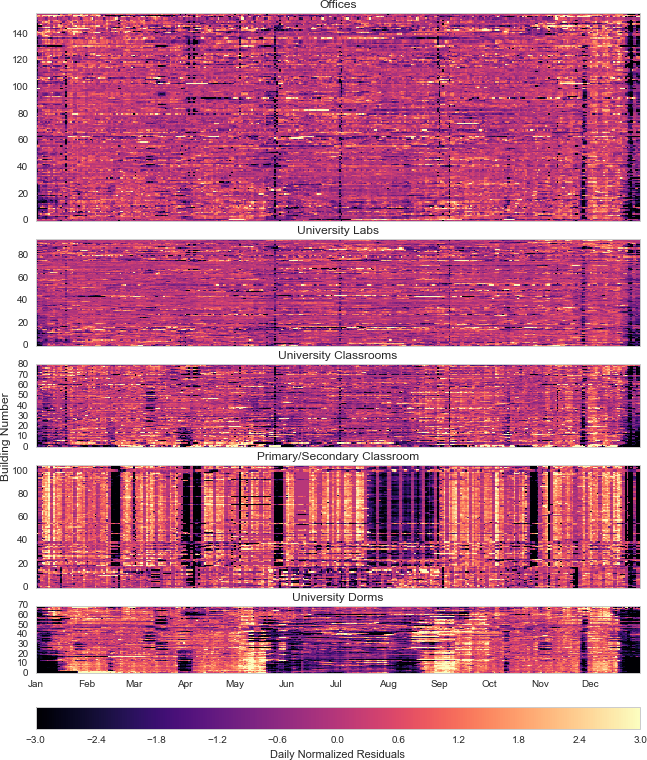
\includegraphics[width=1\columnwidth]{figures/loadshape_heatmap/loadshape_heatmap}
\caption{Heatmap of normalized daily residuals for all case study building
\label{fig:loadshape_all}%
}
\end{center}
\end{figure}

Figures \ref{fig:cooling_heatmap} and \ref{fig:heating_heatmap} illustrate heating and cooling energy regression for all case study buildings. These figures have been normalized according to floor area. Each building's response to outdoor air temperature is indicative of the type of systems installed in addition to the efficiency of energy conversion of those systems. Approximately 15-20\% of offices, labs, and classrooms have a certain amount of cooling electrical consumption, while the rest have little to none. Many of those buildings are on district heating and cooling systems, therefore, weather dependent electrical consumption is likely due to air distribution systems or auxiliary pumps. Several of the labs have year-round cooling consumption, likely due to climate and the high internal loads that accompany laboratory environments.

\begin{figure}[ht!]
\begin{center}
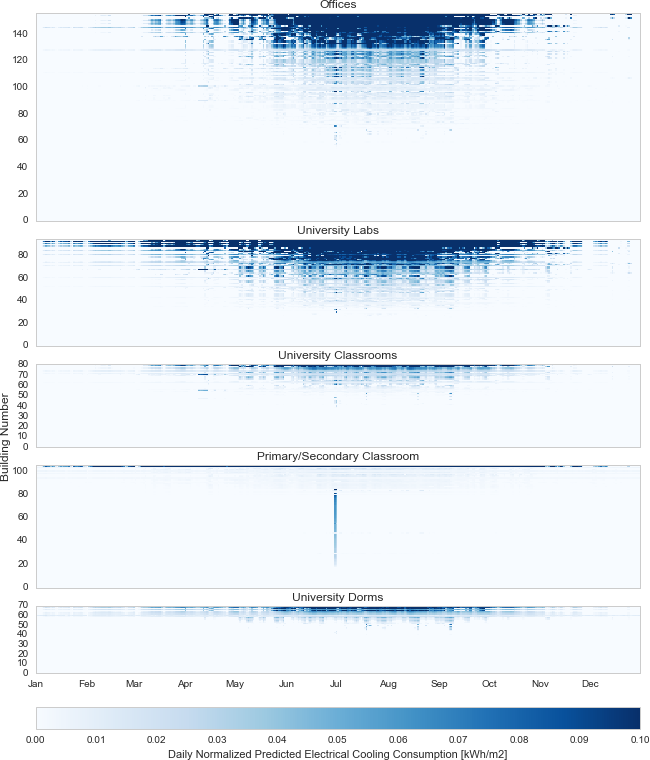
\includegraphics[width=1\columnwidth]{figures/cooling_heatmap/cooling_heatmap}
\caption{Heatmap of normalized predicted electrical cooling energy for all case study buildings
\label{fig:cooling_heatmap}%
}
\end{center}
\end{figure}

\begin{figure}[ht!]
\begin{center}
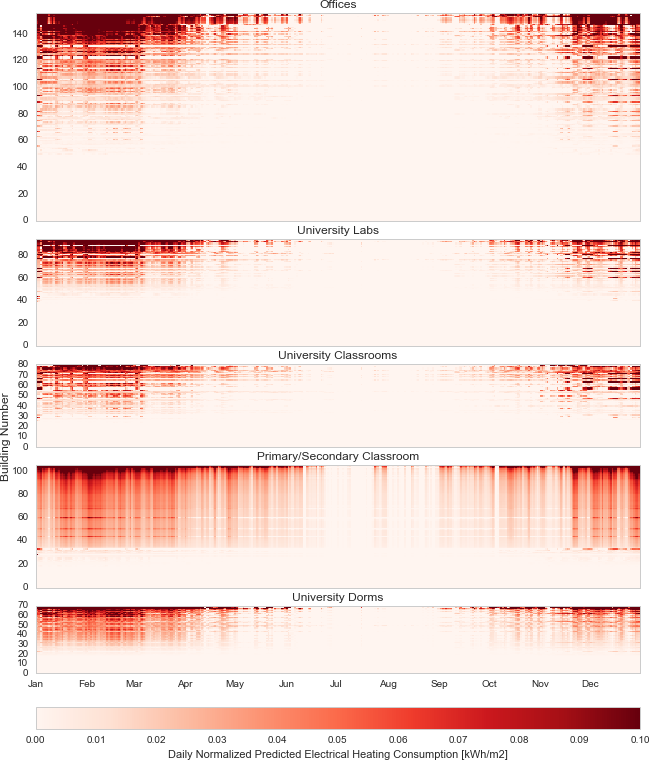
\includegraphics[width=1\columnwidth]{figures/heating_heatmap/heating_heatmap}
\caption{Heatmap of normalized predicted electrical heating energy for all case study buildings
\label{fig:heating_heatmap}%
}
\end{center}
\end{figure}


Figure \ref{fig:weeklypattern_heatmap} illustrates the weekly pattern decomposition for all of the case study buildings. For offices, most of the other cases also exhibit a typical Monday to Friday schedule, with a few exceptions that have various weekday differences and several that have higher values on Saturday. Tuesday seems to be the most consistent across the range of buildings on the peak day of consumption. University labs and classrooms appear to have the same amount of diversity and a similar schedule to offices, perhaps with slightly less use of Fridays. Primary/Secondary school classrooms appear to be the most consistent in their weekly Monday to Friday schedule and have an entirely consistent lack of Saturday and Sunday utilization. University dormitories are the most diverse in their weekly patterns with approximately half of the buildings having dominant weekday schedules and half having dominant weekend schedules.

\begin{figure}[ht!]
\begin{center}
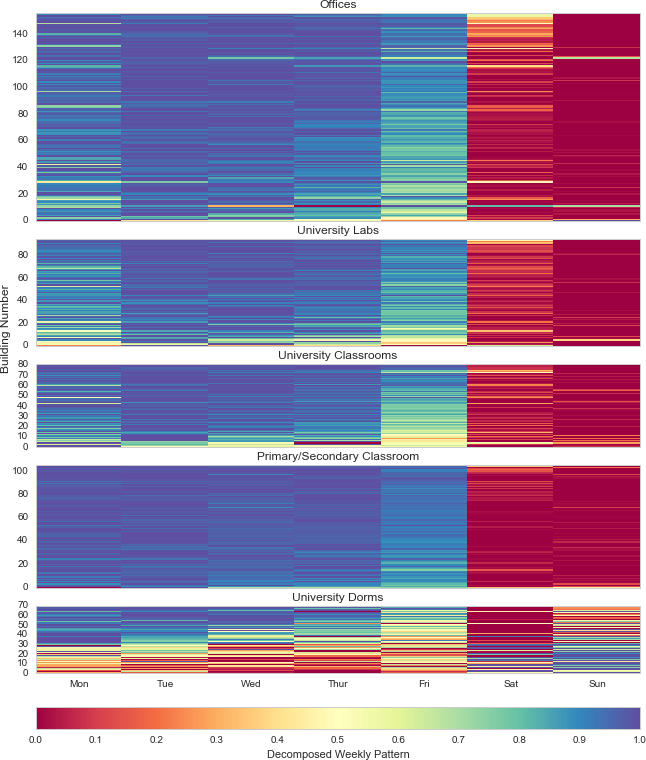
\includegraphics[width=1\columnwidth]{figures/stl_weathernorm_weeklypattern_heatmap/stl_weathernorm_weeklypattern_heatmap}
\caption{Heatmap of decomposed weekly patterns for all case study buildings
\label{fig:weeklypattern_heatmap}%
}
\end{center}
\end{figure}


Figure \ref{fig:trend_heatmap} illustrates the trend decomposition as applied to the entire case study set of buildings. Offices appear to have quite a bit of diversity over time, with a few observable systematic low spots in the spring and autumn periods at the bottom of the heat map. Laboratories reflect that behavior, while university visually has an opposite effect with lower than the average trend in the summer months. Primary/Secondary school classrooms have a very distinct delineation between when school is in session and out of session during the summer and various breaks. As many of these schools are in the UK, their out-of-session periods appear to line up naturally. University dormitories also have clear delineations between occupied and unoccupied periods and they seem also to match up quite well, despite the diversity of data sources of these buildings.

\begin{figure}[ht!]
\begin{center}
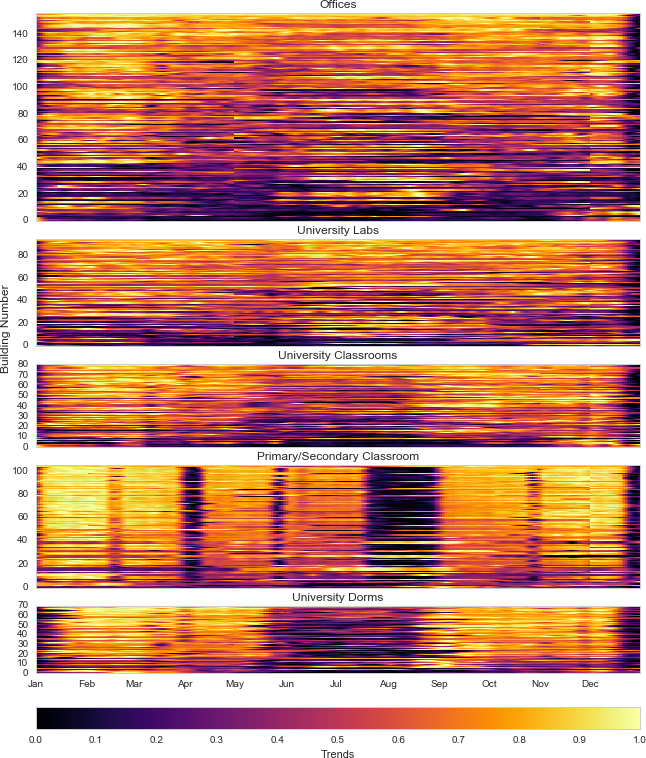
\includegraphics[width=1\columnwidth]{figures/stl_weathernorm_trend_heatmap/stl_weathernorm_trend_heatmap}
\caption{Heatmap of decomposed trend over time for all case study buildings
\label{fig:trend_heatmap}%
}
\end{center}
\end{figure}

Figure \ref{fig:residuals_heatmap} illustrates the residuals applied across all of the case study buildings. Some similarity between all of the university offices, labs, and classrooms are apparent regarding the holidays detected. The most consistent ones include the American memorial day in May, American Independence Day in July, Thanksgiving in November and Christmas Day in December. However, University Labs have a slightly less dramatic range of values. Primary/Secondary schools have appeared to have many more dramatic differences from the \emph{STL} model. 

\begin{figure}[ht!]
\begin{center}
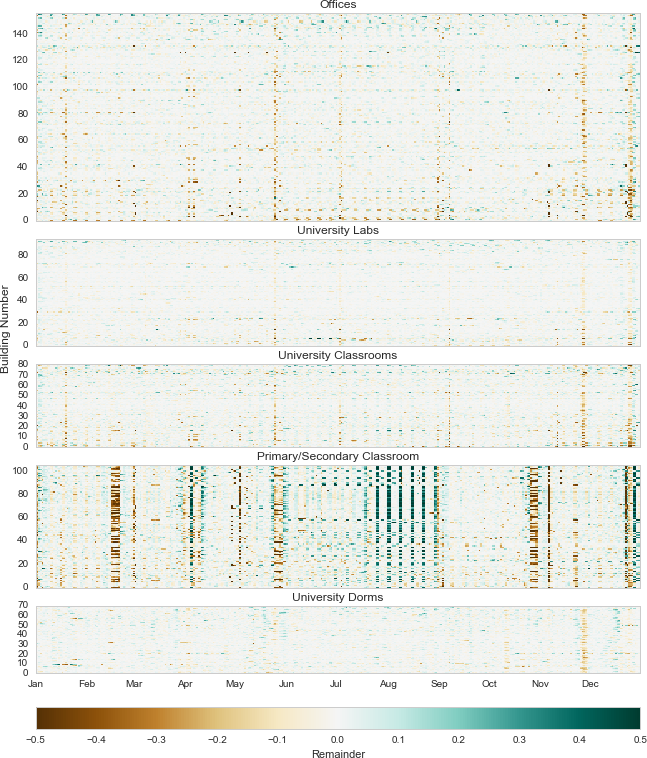
\includegraphics[width=1\columnwidth]{figures/stl_weathernorm_remainder_heatmap/stl_weathernorm_remainder_heatmap}
\caption{Heatmap of decomposed remainder residuals for all case study buildings
\label{fig:residuals_heatmap}%
}
\end{center}
\end{figure}

Overall, model-based temporal features are good at highlighting several different phenomena occurring in a building's behavior. The first, and most important, is essentially how \emph{predictable} a building is across an annual time range and what systematically anomalous days are occurring, such as holidays and break periods. Weather-related models are helpful in understanding what consumption is likely due to heating and cooling systems. This feature is different than the spearman coefficient from the statistic-based section in that it provides more information related to \emph{when} a building goes into climate control modes regarding outside air temperature.
\chapter{Pattern-based Features}
\label{sec:patternbasedfeatures}

Temporal data mining for performance monitoring focuses on the extraction of patterns and model building of time series data. These techniques are, in some ways, similar to many existing building performance analysis approaches; however, different concepts and terminology are used. Two key concepts to understand when applying data mining to buildings are that of \emph{motifs} and \emph{discords}. A motif is a common subsequence pattern that has the highest number of non-trivial matches \citep{patel_mining_2002}, thus, a pattern that is frequently found in the dataset. A discord, on the other hand, is defined as a subsequence of a time series that has the largest distance to its nearest non-self match \citep{keogh_hot_2005}. It is a subsequence of a univariate data stream that is least like all other non-overlapping subsequences and is, therefore, an unusual pattern that diverges from the rest of the dataset. These definitions are more general than that of a \emph{fault} and therefore more appropriate for the goal of higher level information extraction with less parameter setting. In short, the goal is to find \emph{interesting or infrequent} behavior efficiently and not create a detailed list of specific problems that could be occurring in individual systems.

\section{Theoretical Basis}
\label{sec:patternbasedtheory}

To work with standard temporal mining approaches, Symbolic Aggregate approXimation (SAX) representation of time-series data \citep{lin_symbolic_2003} is used. SAX allows discretization of time series data which facilitates the use of various motif and discord detection algorithms. The process breaks time series data into subsequences which are converted into an alphabetic symbol. These symbols are combined to form strings to represent the original time series enabling various mining and visualization techniques. Regarding application, an example of a process using SAX-based techniques is the VizTree tool that uses augmented suffix tree visualizations designed for usability by an analyst \citep{lin_visually_2004}. A particular application of VizTree is the analysis of collected sensor data from an impending spacecraft launch in which thousands of telemetry sensors are feeding data back to a command center where experts are required to interpret the data. Visualization and filtering tools are needed that allow a natural and intuitive transfer of mined knowledge to the monitoring task. Human perception of visualizations and the algorithms behind them must work in unison to achieve an understanding of significant amounts of original data streams. 

% SAX has been used on building performance data before in a few studies focused on data center chilled water plants and it was found useful in detecting the most efficient control strategies \citep{Patnaik:2009uk}. The same research was used to create a visual exploration tool for high-frequency time series data \citep{Hao:2012go}. Despite these efforts, our review of the literature found a lack of tools or processes similar to the VizTree tool for day-types that fit in our targeted context of bridging the performance gap. We will introduce a new process focused on combining temporal approximation, filtering, and visualization.

\subsection{Dirunal Pattern Extraction}
\label{sec:dayfilter}

Towards the development of diurnal motif and discord extraction, a new technique was developed as an application of temporal data mining to building performance data. It is a process called \emph{DayFilter} and it includes five steps designed to filter structure incrementally from daily raw measured performance data. These steps, as seen in Figure~\ref{fig:process}, are intended to bridge the gap between contemporary top-down and bottom-up techniques. The arrows in the diagram denote the execution sequence of the steps. Note that steps 3, 4, and 5 produce results applicable to the implementation of bottom-up techniques. Much of the graphics and explanation for this section are contained in a publication explaining DayFilter and its uses \citep{miller_automated_2015}.

The whole building and subsystem metrics are targeted for analysis to determine high-level insight. The process begins with a data preprocessing step which removes obvious point-based outliers and accommodates for gaps in a univariate data set of variable length. Next, the raw data is transformed into the SAX time-series representation for dimensionality reduction by creating groups of SAX words from daily windows. This step enables the quick detection of \emph{discords}, or regular patterns of performance that fall outside what is considered normal in the dataset according to the frequency of patterns. The discords are filtered out for future investigation while the remaining set of SAX words is clustered to create performance \emph{motifs} or the most common daily profiles. The additional clustering step beyond the SAX transformation and filtering adds the ability further to aggregate daily profiles beyond the SAX motif candidates. These clusters are useful in characterizing what can be considered \emph{standard} performance. Finally, these data are presented using visualization techniques as an aid to interpreting the questionable discords and the common clusters. In the following simplified example, each of these steps is detailed. The input parameter selections in this section are based on suggestions from other studies using SAX aggregation and clustering approaches. 
% Additional discussion of parameter selection is presented in Section \ref{sec:parameters}.

\begin{figure}[ht!]
\begin{center}
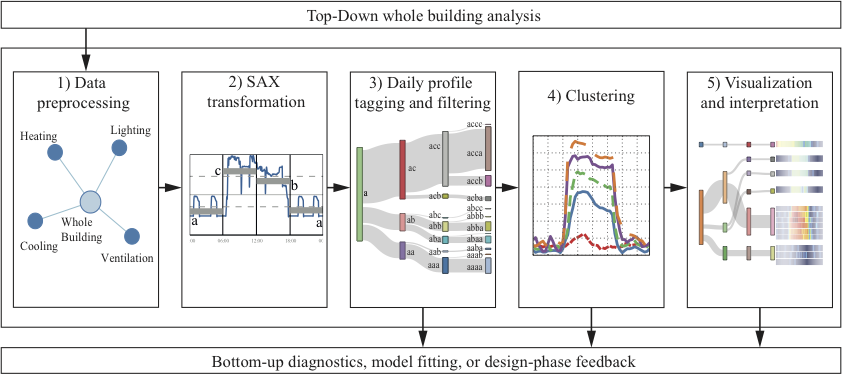
\includegraphics[width=1\columnwidth]{figures/ClusteringProcessDiagram_V4/ClusteringProcessDiagram_V4}
\caption{Diagram of the five steps in the \emph{DayFilter} (from \citep{miller_automated_2015})
\label{fig:process}%
}
\end{center}
\end{figure}

As in any data mining approach, data preprocessing is an important step to clean and standardize the data. In the proposed method, extreme point measurements are removed that fall outside of three standard deviations, 3$\sigma$, of the mean, $\mu$, of the selected univariate data stream $x(t)$. The data are then normalized to create a dataset, $Z(t)$ with an approximate 0 mean and a standard deviation of close to 1 \citep{goldin_similiarity_1995}:

\begin{equation}
Z(t)=\frac{x(t) -\mu}{\sigma}
\end{equation}
% ,i \in N$$

In the second step, $Z(t)$ is transformed into a symbolic representation using SAX. It is one of the many means of representing time-series data to enhance the speed and usability of various analysis techniques. SAX is a type of Piecewise Aggregate Approximation (PAA) representation developed by Keogh et. al and it has been used extensively in numerous applications \citep{lin_experiencing_2007}. 

In brief, the SAX transformation is as follows. The normalized time-series, $Z(t)$, is first broken down into $N$ individual non-overlapping subsequences. This step is known as \emph{chunking}, and the period length $N$ is based on a context-logical specific period \citep{lin_visualizing_2005}. In this situation, $N$ is chosen as 24 hours due to the focus on daily performance characterization.  Each chunk is then further divided into $W$ equal sized segments. The mean of the data across each of these segments is calculated and an alphabetic character is assigned according to where the mean lies within a set of vertical breakpoints, $B=\beta_1,...,\beta_{a-1}$. These breakpoints are calculated according to a chosen alphabet size, $A$, to create equiprobable regions based on a Gaussian distribution, as seen in Table~\ref{fig:SAXBreakpoints}.

\begin{figure}[ht!]
\begin{center}
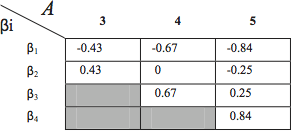
\includegraphics[width=0.42\columnwidth]{figures/SAXBreakpoints/SAXBreakpoints}
\caption{Example breakpoint lookup table from Keogh et. al \citep{keogh_hot_2005} for $A$ = 3, 4, 5 calculated from a Gaussian distribution \citep{miller_automated_2015}
\label{fig:SAXBreakpoints}%
}
\end{center}
\end{figure}

Based on a chosen value of $W$ segments and alphabet size $A$, each $N$ size window is transformed into a SAX \emph{word}. An example of this process is seen in Figure~\ref{fig:SAXWord}. This example shows two daily profiles which are converted to the SAX words, \emph{acba} and \emph{abba}. The SAX word is useful from an interpretation point of view in that each letter corresponds consistently to a subsequence of data from the daily profile. For example, the first letter explains the relative performance for the hours of midnight to 6:00 AM. Therefore if the size of $A$ is set to 3, a SAX word whose first letter is $a$ would have low, $b$ would indicate average, and $c$ would correspond to high consumption. Larger sizes of $A$ would create SAX words with a more diverse range of characters and would capture more resolution magnitude-wise.

\begin{figure}[ht!]
\begin{center}
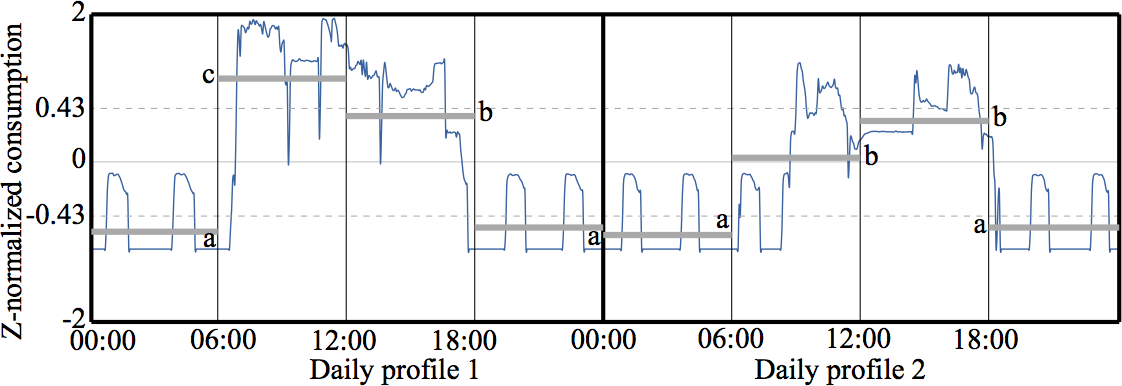
\includegraphics[width=0.7\columnwidth]{figures/SAXCreationV2/SAXCreationV2}
\caption{SAX word creation example (based on figure from Keogh et. al \citep{keogh_hot_2005}) of two days of 3 minute frequency data, parameters are $N$=480, $W$=4, and $A$ = 3 and the generated representative word for daily profile 1 is \emph{acba} and daily profile 2 is \emph{abba} (from \citep{miller_automated_2015})
\label{fig:SAXWord}%
}
\end{center}
\end{figure}

The individual subsequences, $N$, are not normalized independently. This particular decision is divergent from the generalized shape-based discord approaches and is because, at this level of analysis and the context of building performance data, there is interest in discovering interesting subsections based on both magnitude and shape. 
% used with permission from Keogh et. al \citep{Keogh:2005wd}.

The targeted benefits of using SAX in this scenario are that discretization uniformly reduces the dimensionality and creates sets of words from the daily data windows. This transformation allows the use of hashing, filtering, and clustering techniques that are commonly used to manipulate strings \citep{lin_experiencing_2007}. 

Once the SAX words are created, each pattern is visualized and tagged as either a motif or discord. The results of applying the SAX process to a two-week sample power dataset are shown in Figure~\ref{fig:saxcreation}. The diagram shows how each daily chunk of high-frequency data is transformed into a set of SAX characters. In this example, an alphabet size, $A$, of 3 and a subsequence period count, $W$, of 4 are used for each character aggregating the data from 6 hours of each profile. These parameters are the same as used in the more simplified two-day example from Figure~\ref{fig:SAXWord}

\begin{figure}[ht!]
\begin{center}
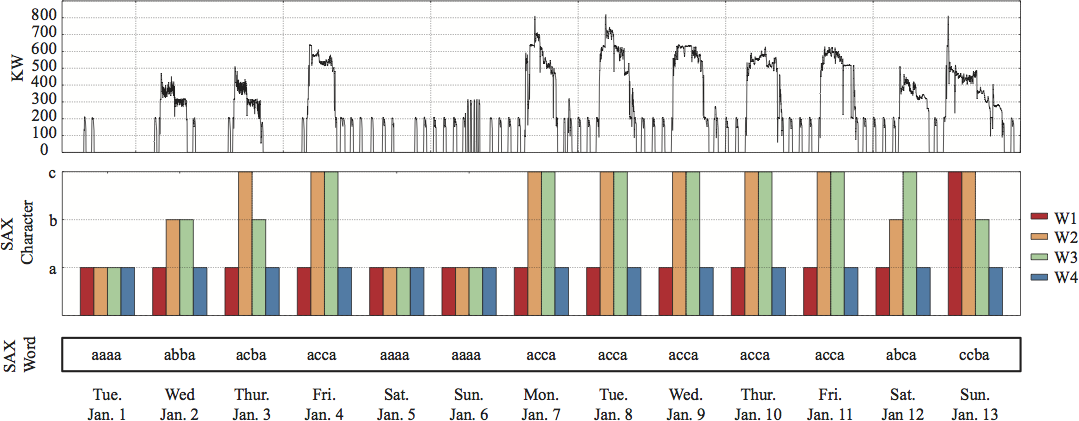
\includegraphics[width=1\columnwidth]{figures/SAXWordExample_BarLine/SAXWordExample_BarLine}
\caption{Creation of SAX words from daily non-overlapping windows: W1: 00:00-06:00, W2: 06:00-12:00, W3: 12:00-18:00, W4: 18:00-24:00. Time series data is transformed according to a SAX character creation and then as a string, or SAX word \citep{miller_automated_2015}
\label{fig:saxcreation}%
}
\end{center}
\end{figure}

Figure~\ref{fig:saxdiscordsankey} visualizes the frequency of the SAX strings and substrings in the form of an augmented suffix tree. Suffix trees have been an integral part of string manipulation and mining for decades \citep{weiner_linear_1973}. Augmented suffix trees enable a means of visualizing the substring patterns to show frequency at each level. This figure incorporates the use of a Sankey diagram to visualize the tree with each substring bar height representing the number of substring patterns existing through each window of the day-types. The more frequent patterns are categorized as \emph{motifs} or patterns which best describe the average behavior of the system. One can see the patterns with the lower frequencies and their indication as \emph{discords} or subsequences that are least common in the stream.  

Heuristically, a decision threshold is set to distinguish between motifs and discords. This threshold can be based on the word frequency count for each pattern as a percentage of the number of all observations. This threshold can be tuned to result in a manageable number of discord candidates to be further analyzed. More details about setting this limit will be discussed the applied case studies.

% The extracted SAX words are grouped according to frequency and a threshold is chosen to differentiate the profiles to consider as motif candidates or as low-frequency day types to tag for further investigation.

In the two-week example, this process yields two patterns which have a frequency greater than one and thus are the motif candidates. A manual review of the data confirms that those patterns match with an expected profile for a typical weekday ($acca$) and weekend ($aaaa$). The less frequent patterns are tagged as discords and can be analyzed in more detail. In this case, it can be determined that the patterns $abba$, $abca$, and $acba$, despite being infrequent, are not abnormal due to the occupancy schedule for those particular days. Pattern $ccba$, however, is not explainable within the scheduling and is due to a fault causing excessive consumption in the early morning hours.

This step leads into the next phase of the process focused on further aggregating the motif candidates of the dataset. The size and number of potential motif filtered in this step will give an indication of the number of clusters that will likely pick up the exact structure from the dataset.

\begin{figure}[ht!]
\begin{center}
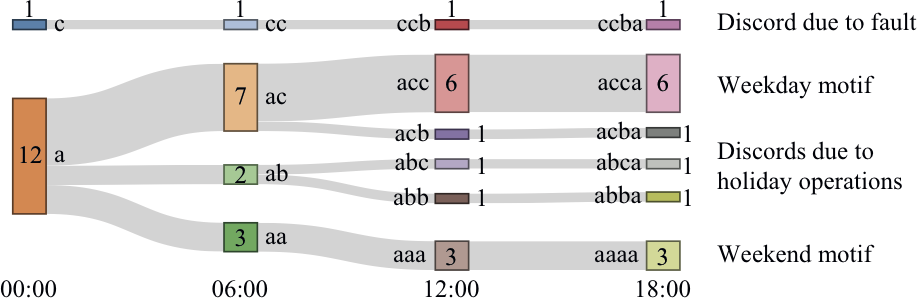
\includegraphics[width=0.84\columnwidth]{figures/DiscordSankeyExample/DiscordSankeyExample}
\caption{Augmented suffix tree of SAX words. Each level from left to right represents the $W1-W4$, the substrings are noted adjacent to each bar, and the bar thickness is proportional to the number of days within each pattern type. The pattern frequency in number of days is noted in this graphic within or just adjacent to each bar. (from \citep{miller_automated_2015})
\label{fig:saxdiscordsankey}%
}
\end{center}
\end{figure}

As the final step, interpretation and visualization are critical for \emph{DayFilter} for a human analyst to visually extract knowledge from the results, and to make decisions regarding further analysis. The \emph{Overview, zoom and filter, details-on-demand} approach \citep{shneiderman_eyes_1996} and the previously mentioned VizTree tool \citep{lin_visually_2004} are used for insight into this process. The hidden structures of building performance data are revealed through the SAX process, and visualization is used to communicate this structure to an analyst. The method uses a modified Sankey diagram to visualize the augmented suffix tree in a way which the count frequency of each SAX word can be distinguished.  Figure~\ref{fig:saxdiscordsankeyheatmap} shows how this visualization is combined with a heat map of the daily profiles associated with each of the SAX words using the same two-week example data from Figures \ref{fig:saxcreation} and \ref{fig:saxdiscordsankey}. The Sankey diagram is rearranged according to the frequency threshold set to distinguish between the motif and discord candidates.

In Figure~\ref{fig:saxdiscordsankeyheatmap}, the discords are shown as the top four days, Jan. 2, 3, 12, and 13 and the remaining days are shown as more frequent potential motifs below. Each daily profile is shown adjacent to the right of the Sankey diagram and is expressed as a color-based heatmap. Each horizontal bar of the heat map is an individual day, and they are grouped according to pattern with the associated legend informing the viewer the magnitude of energy consumption across the day. This visualization is designed to present quickly the patterns arranged according to a sort of hierarchy provided by the suffix tree. One can more easily distinguish seemingly \emph{normal} versus \emph{abnormal} behavior with this combination of visualizations. 

\begin{figure}[ht!]
\begin{center}
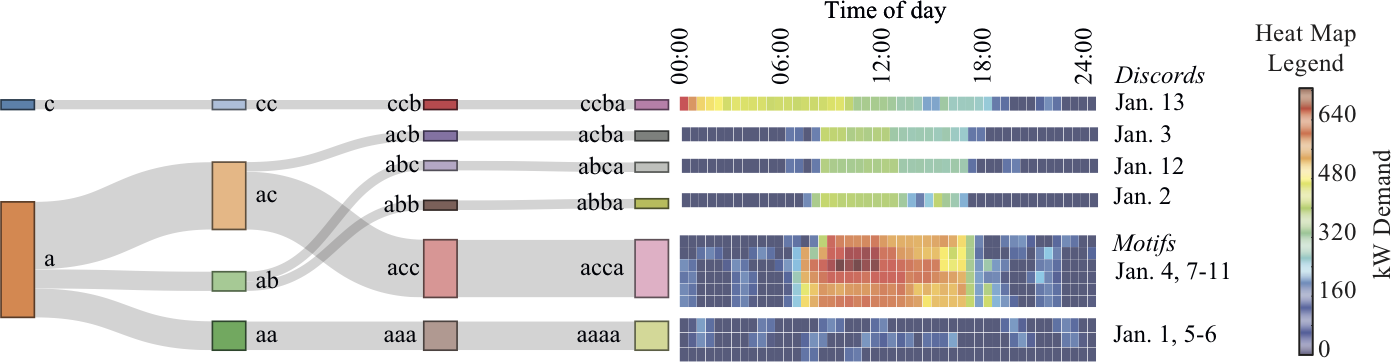
\includegraphics[width=1\columnwidth]{figures/DiscordSankeyExampleWithHeatmapV2/DiscordSankeyExampleWithHeatmapV2}
\caption{Example suffix tree with heatmap from the two week dataset. The sankey diagram illustrates the divisions according to pattern and the general categories of motif vs. discord candidates. Each horizontal line in the heatmap represents a single daily profile to illustrate consumption magnitude of each SAX word. \citep{miller_automated_2015}
\label{fig:saxdiscordsankeyheatmap}%
}
\end{center}
\end{figure}

\emph{DayFilter} is applied on a large energy performance datasets to demonstrate the usability and results in real-life scenarios. The process is applied to a 70,000 square meter international school campus in the humid, tropical climate of Singapore. It was built in 2010 and includes a building management system (BMS) with over 4,000 measured data points taken at 5-minute intervals from the years of 2011-2013 - resulting in close to 800 million records of raw data. This collection includes 120 power meters and 100 water meters in the energy and water management system. The data from this study are a seed dataset in an open repository of detailed commercial building datasets \citep{miller_seed_2014}. 

The chilled water plant electricity consumption is targeted in this case due to its importance in this climate and the potential savings opportunities available through chilled water plant optimization. Measured kilowatt-hour (kWh) and kilowatt (kW) readings were taken from July 12, 2012, to October 29, 2013, with 474 total daily profiles analyzed. Figure~\ref{fig:sankeyheatmap1} illustrates a Sankey diagram with a heat map of the output of the \emph{DayFilter} process with parameters set to $A$=3 and $W$=4. The discord and motif candidates are separated in this case according to a decision threshold which quantifies a discord as a day-type with a frequency count less than 2\% of total days available. This distinction results in 39 days with patterns tagged as discord candidates, which is 8.2\% of the total days in the dataset. 

\begin{figure}[ht!]
\begin{center}
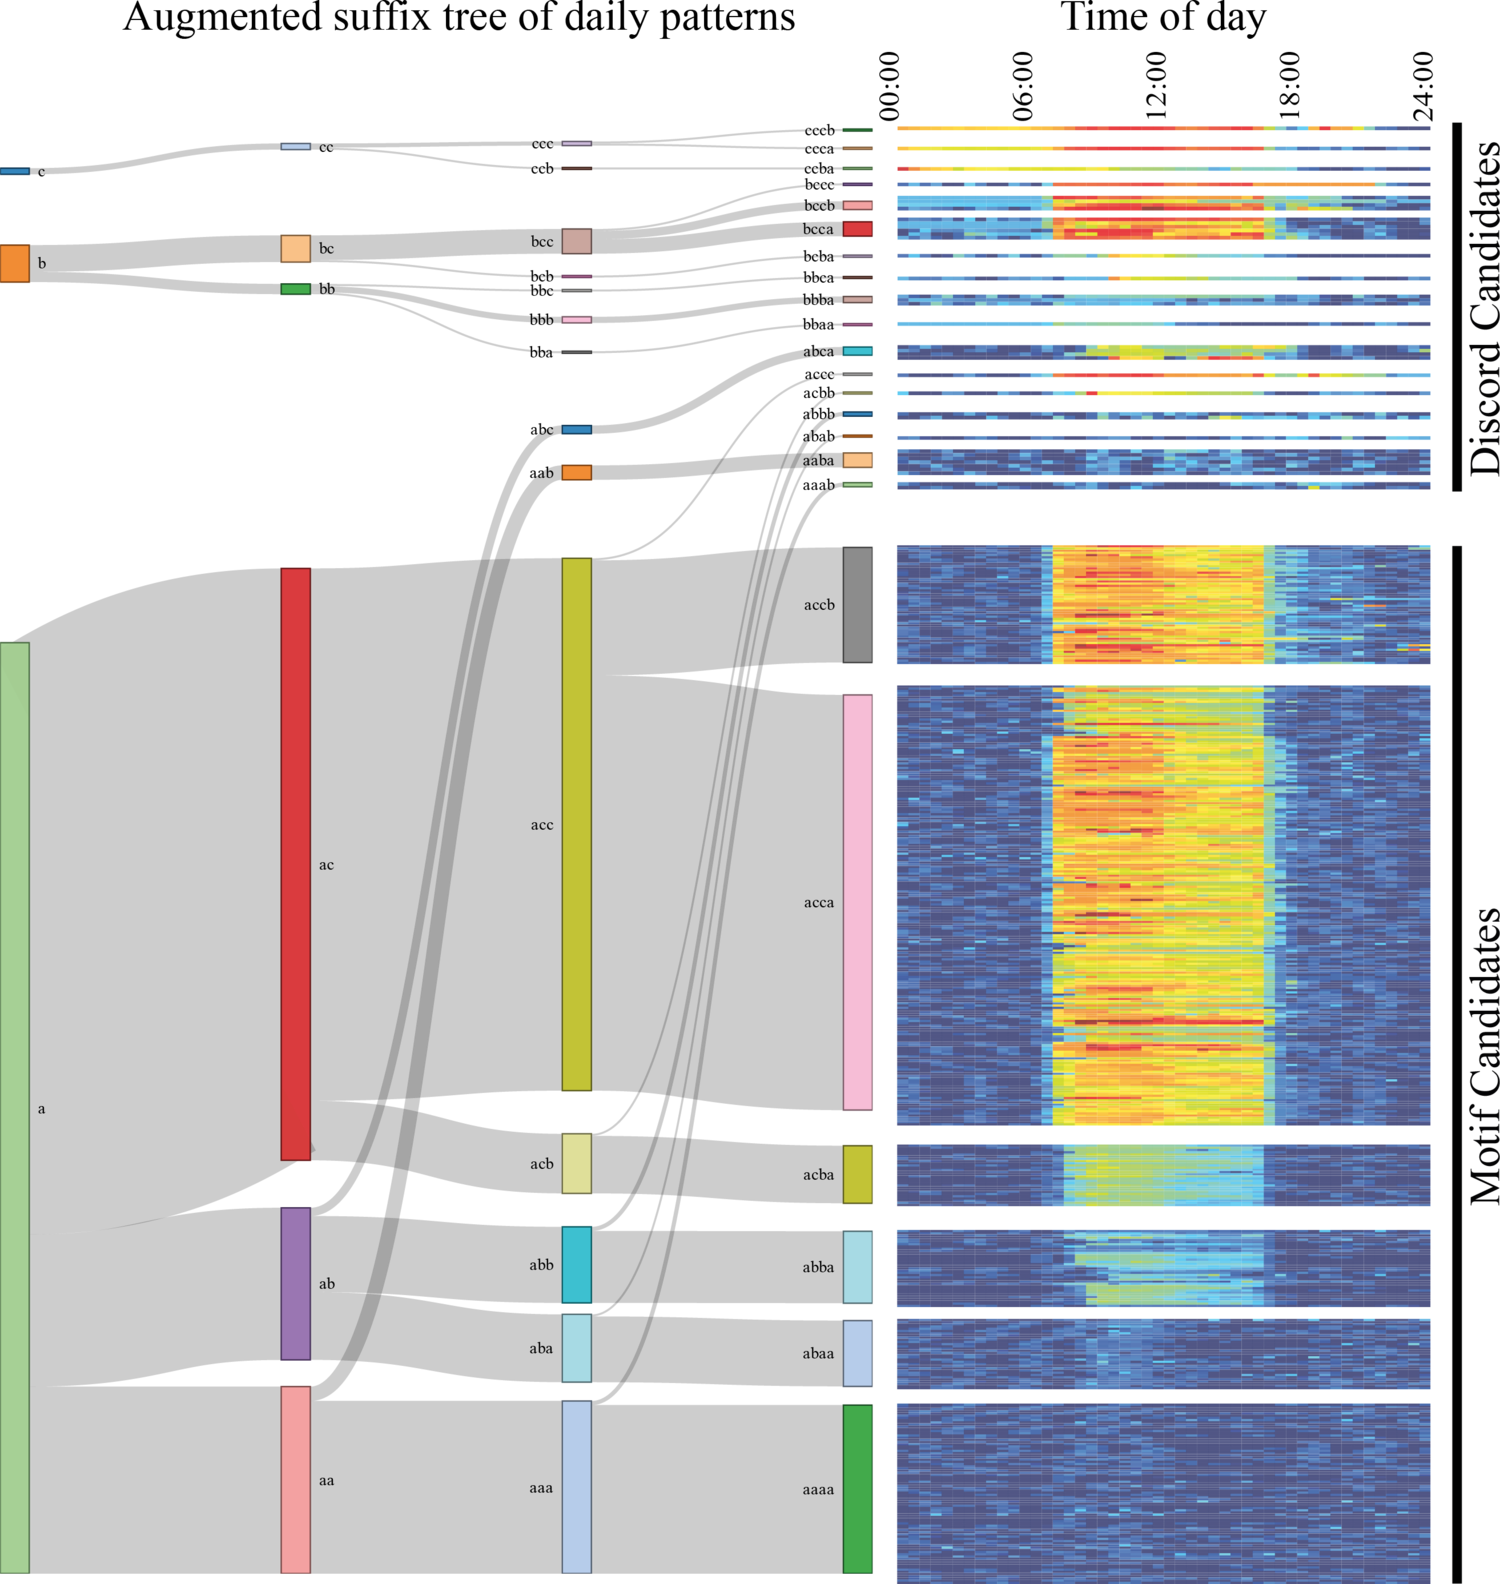
\includegraphics[width=1\columnwidth]{figures/UWC_Chiller_SankeyHeatmapV2/UWC_Chiller_SankeyHeatmapV2}
\caption{Cooling electricity consumption representation of the day-types from the DayFilter process \citep{miller_automated_2015}
\label{fig:sankeyheatmap1}%
}
\end{center}
\end{figure}

In general, there are six primary motif candidates with two candidates appearing to be typical weekday types, two holiday or half-capacity types, and two-weekend unoccupied types. Pattern $aaaa$ and $abaa$ are predominantly flat profiles common to non-occupied cooling consumption. Patterns $abba$ and $acba$ are representative of days in which school is out of session, but staff still occupies the office spaces. Pattern $acca$ represents a regular full-occupied school day, and it is by far the most common with 202 days tagged out of 474. Pattern $accb$ is similar to $acca$ with slightly more use in the late afternoon and early evening. This phenomenon is due to extracurricular activities planned outside the normal operating schedule of the facility.

For characterization, a metric is developed from the \emph{DayFilter} process that approximates the presence of motifs and discords. This metric is a daily frequency calculation of each day's pattern count versus the total number of days. An example of this metric is seen in Figure \ref{fig:dayfilter_single}.

\begin{figure}[ht!]
\begin{center}
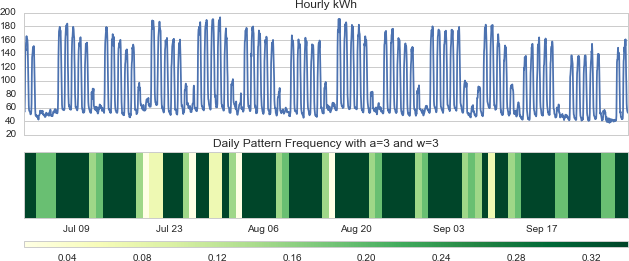
\includegraphics[width=1\columnwidth]{figures/dayfilter_example1/dayfilter_example1}
\caption{Single building example of daily pattern frequency using \emph{DayFilter}, a=3 and w=3
\label{fig:dayfilter_single}%
}
\end{center}
\end{figure}

\subsection{Pattern Specificity}
\label{sec:patternspec}

Another way to leverage SAX to characterize the case study data is to use it to extract which patterns are most indicative of a particular building use type. This information is obtained using the SAX-VSM process pioneered by Senin and Malinchik that uses SAX and Vector Space Model technique from the text mining field \citep{Senin_2013}. Conventionally this method is utilized as a classification model to predict which class a certain time-series belongs. A by-product of the process is that the subsequences of each data stream are assigned a metric indicating their specificity. Pattern specificity is a concept that quantifies how well a meter \emph{fits within its class}. This technique is used to determine whether a building is operating similar to other supposed peer buildings of the same type.

The SAX-VSM process begins with the SAX word creation, similar to \emph{DayFilter} as shown in Figure \ref{fig:saxcreation}. However, the key difference is that the conventional SAX process extracts word patterns from overlapping windows as opposed to simply \emph{chunking} each daily profile. Each data stream within a particular class of a training data set is converted to SAX words using the same input variables of alphabet size, $A$, and subsequence period count, $W$. In addition, a $P$ variable is chosen to indicate the size of the sliding window. With SAX-VSM, all of the SAX words for a certain use type class, such as Offices, are then combined into a large Bag of Words (BOG) representation called a corpus, and then used to build a term frequency matrix. This model is then used to calculate a $tf*idf$ weight coefficient, which is the product of the term frequency ($tf$) and the inverse document frequency ($idf$). The term frequency is a logarithmically scaled metric based on the incidence of a pattern in the BOG. The inverse document frequency is computed as the log of the ratio of the number of classes to the number of bags where each pattern occurs \citep{Manning}. Once this matrix of weight vectors is computed, the cosine similarity of an individual data stream can be calculated to determine how similar to each class it is. 

\begin{figure}[ht!]
\begin{center}
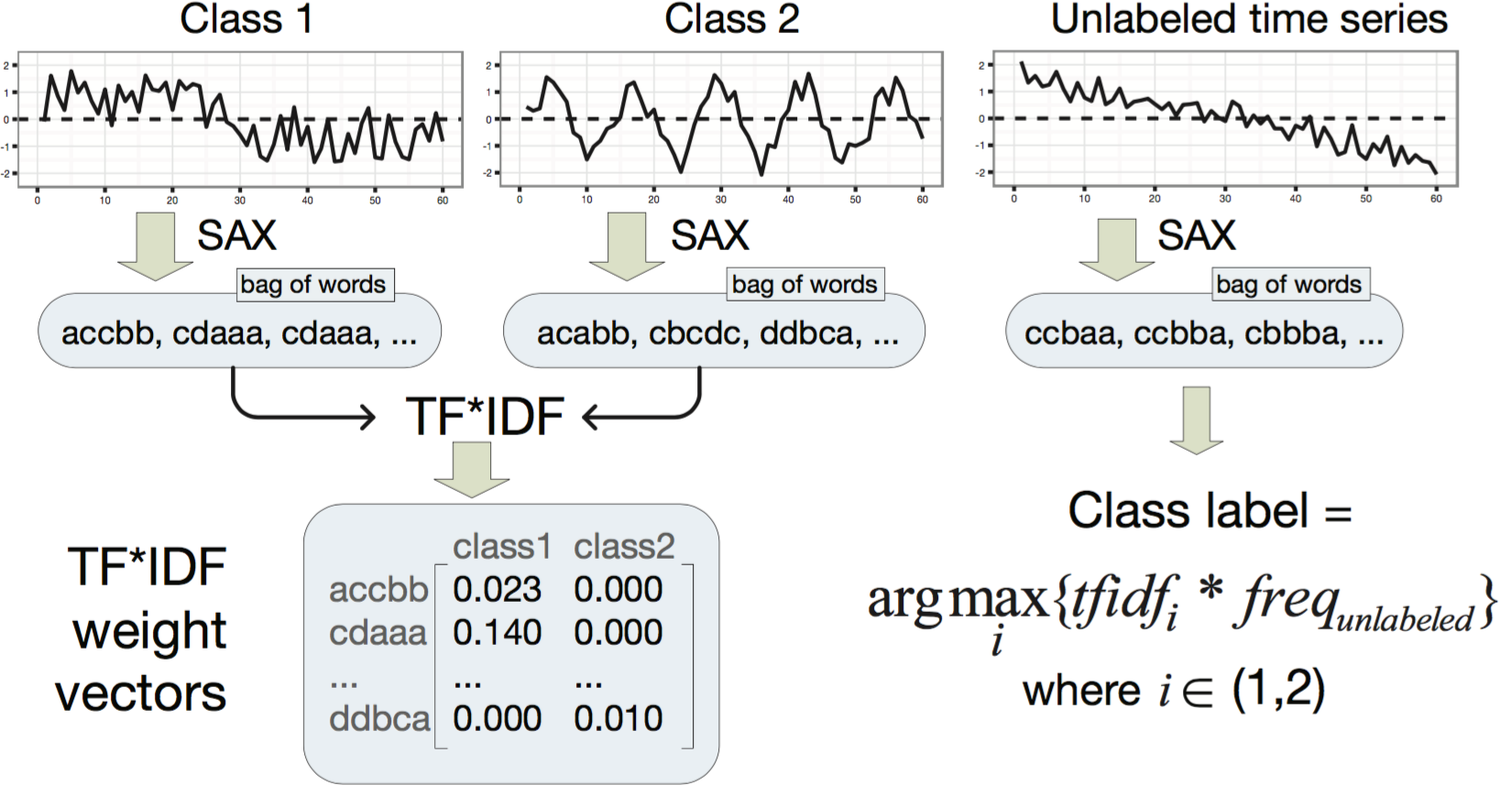
\includegraphics[width=0.98\columnwidth]{figures/jmotif/jmotif}
\caption{Overview of SAX-VSM algorithm: first, labeled time series are converted into bags of words using SAX; secondly, $tf*idf$ statistics is computed resulting in a single weight vector per training class. For classification, an unlabeled time series is converted into a term frequency vector and assigned a label of a weight vector which yields a maximal cosine similarity value (figure and caption used with permission from \citep{senin_sax-vsm:_2013}).
\label{fig:saxvsm_overview}%
}
\end{center}
\end{figure}

In this study, the goal is not to use SAX-VSM to classify each data stream, but to extract instead temporal features that can be used to characterize them. Thus, the in-class cosine similarity is calculated for each building's data set as compared to the class it was assigned. This process is not conventional from the classification sense as it is considered over-fitting due to all samples being included in the training set. This situation is tolerated in this analysis as it is desired to quantify only how much the patterns of use for a building compare to those of its labeled \emph{peers}.

The specificity metric for each data stream is calculated for each sliding window by subtracting all other $tf*idf$ weights for each pattern from the in-class weighting. An example of this weighting

\begin{figure}[ht!]
\begin{center}
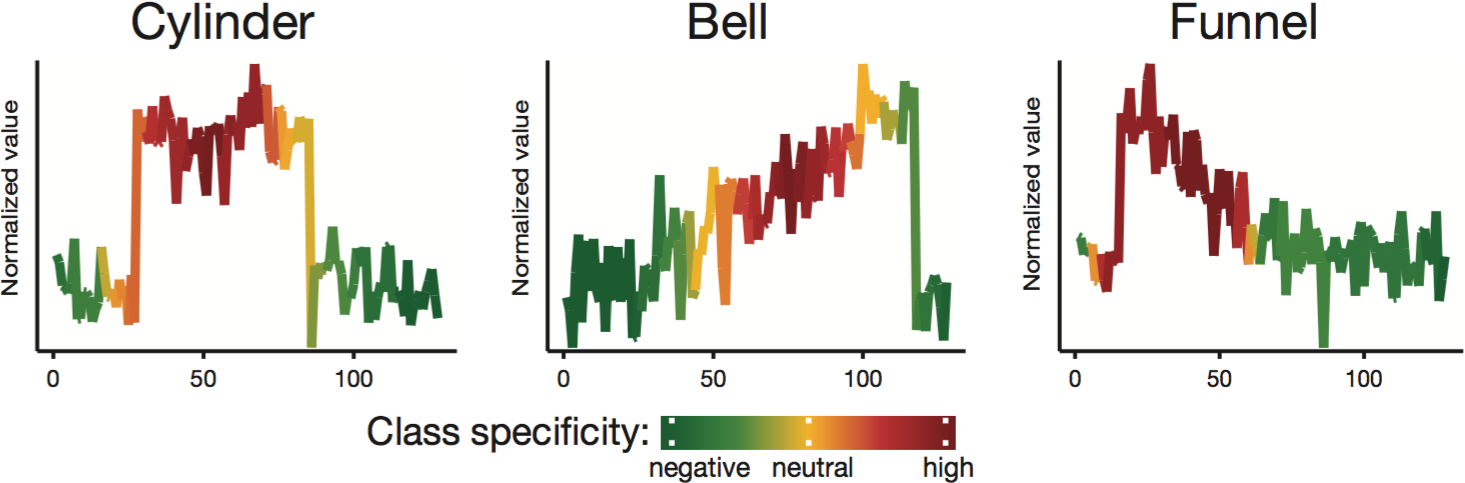
\includegraphics[width=1\columnwidth]{figures/jmotif_tfidfspec/jmotif_tfidfspec}
\caption{An example of the heat map-like visualization of subsequence \emph{importance} to a class identification. Color value of each point was obtained by combining $tf*idf$ weights of all patterns which cover the point. The highlighted class specificity corresponds to a sudden rise, a plateau, and a sudden drop in Cylinder; to a gradual increase in Bell; and to a sudden rise followed by a gradual decline in Funnel (figure and caption used with permission from \citep{senin_sax-vsm:_2013})
\label{fig:specificity_example}%
}
\end{center}
\end{figure}

The specificity calculation process is implemented on each of the building test data sets. A single building example of this process is seen in Figure \ref{fig:dailyspecificity_single}. This building is within the \emph{Office} use-type classification; thus the color spectrum indicates how precise each subsequence is to this building's behavior as an office as compared to the entire training data set. This example is using the input metrics of $a=8$, $p=8$, and $w=24$ to capture the specificity of daily patterns. These parameters settings include the use of a 24-hour sliding window that is divided into eight segments of three hours length, and the normalized magnitude assigns a symbol from a range of eight letters, $a,b,c,d,e,f,g,h$.

\begin{figure}[ht!]
\begin{center}
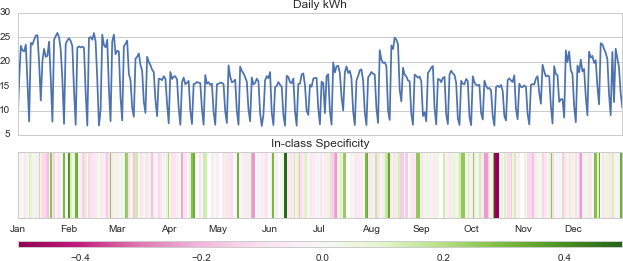
\includegraphics[width=1\columnwidth]{figures/jmotif_alldatatrained_dailyspecificity_example_24_8_8/jmotif_alldatatrained_dailyspecificity_example_24_8_8}
\caption{Single building example of daily in-class specificity, a=8, p=8, and w=24 for an office building. Positive specificity indicates behavior that is characteristic of a certain class, while negative values indicates behavior of a different class.
\label{fig:dailyspecificity_single}%
}
\end{center}
\end{figure}

The specificity calculation process also implemented using input parameters designed to capture patterns of weekly behavior. In this situation, the input metrics of $a=6$, $p=14$, and $w=168$ are chosen to capture this behavior. These parameters settings model a 168-hour sliding window (one week) that is divided into 14 segments of 12 hours length, and the normalized magnitude assigns a symbol from a range of six letters, $a,b,c,d,e,f$. A single building example is seen in Figure \ref{fig:weeklyspecificity_single}. This building is also within the \emph{Office} use-type classification; thus the color spectrum indicates how precise each weekly subsequence is to this building's behavior as an office as compared to the entire training data set.

\begin{figure}[ht!]
\begin{center}
\includegraphics[width=1\columnwidth]{figures/jmotif_alldatatrained_dailyspecificity_example_168_6_14/jmotif_alldatatrained_dailyspecificity_example_168_6_14}
\caption{Single building example of weekly in-class specificity, a=x, w=X, and p=X
\label{fig:weeklyspecificity_single}%
}
\end{center}
\end{figure}

\subsection{Long-term Pattern Consistency}
\label{sec:patternconsistency}

Breakout detection screening is a process in which each data stream is analyzed according to the tendency to shift from one performance state to another with a transition period in between. This metric is used in this context to quantify long-term pattern consistency, and much of the explanation and graphics in this section are from a previous study \citep{miller_forensically_2015}. Breakout detection is a type of change point detection that determines whether a change has taken place in a time series dataset. Change detection enables the segmentation of the data set to understand the nonstationarities caused by the underlying processes and is used in multiple disciplines involving time-series data such as quality control, navigation system monitoring, and linguistics \citep{basseville_detection_1993}. Breakout detection is applied to temporal performance data to understand general, continuous areas of performance that are similar and the transition periods between them.

In this process, an R programming package, \emph{BreakoutDetection}, is utilized, which is also developed by Twitter to process time-series data related to social media postings\footnote{https://github.com/twitter/BreakoutDetection}. This package uses statistical techniques which calculate a divergence in mean and uses robust metrics to estimate the significance of a breakout through a permutation test. The specific technical details of the breakout detection implementation can be found in a study by James et al. \citep{james2014leveraging}. \emph{BreakoutDetection} uses the E-Divisive with Medians (EDM) algorithm, which is robust amongst anomalies and can detect multiple breakouts per time series. It can identify the two types of breakouts, mean shift and ramp up. Mean shift is a sudden jump in the average of a data stream, and ramp up is a gradual change of the value of a metric from one steady state to another. The algorithm has parameter settings for the minimum number of samples between breakout events that allows the user to modulate the amount of temporal detail.

The goal in using breakout detection for building performance data is to find directly when macro changes occur in sensor data stream. This discovery is particularly exciting in weather-insensitive data to understand when modifications are made to the underlying system in which performance is being measured. Figure \ref{fig:breakout_single} data from a single building data stream. Each color represents a group of continuous, steady-state operation and each change in color is, thus, a breakout. These breakouts could be the result of schedule or control sequence modifications, systematic behavior changes, space use type changes, etc. Creation of diversity factor schedules should target data streams which have few breakouts and the data between breakouts is the most applicable for model input. One parameter setting for breakout detection is the minimum breakout size threshold. This parameter prevents breakouts from being detected to close together, thus capturing potentially noisy behavior for the particular data set.

\begin{figure}[ht!]
\begin{center}
\includegraphics[width=1\columnwidth]{figures/breakout_example/breakout_example}
\caption{Single building example of breakout detection to test for long-term volatility in an university dormitory building. A minimum threshold of 30 days is chosen in this case, which explains the lack of threshold shift in April, a break that may be attributed to spring break for this building
\label{fig:breakout_single}%
}
\end{center}
\end{figure}

\section{Implementation and Discussion}
\label{sec:patternbaseddiscussion}

Figure \ref{fig:dayfilter_all} shows this pattern frequency metric as applied to all the case study buildings. One will notice that there is a range of pattern frequencies occurring across each of the building use types. Offices and Primary/Secondary Classrooms seem to have larger regions of darker, more consistent behaviour. Labs and Classrooms seem to be more volatile across the time ranges.

\begin{figure}[ht!]
\begin{center}
\includegraphics[width=1\columnwidth]{figures/dayfilter_heatmap/dayfilter_heatmap}
\caption{Heatmap of daily pattern frequencies using \emph{DayFilter} with a=3 and w=3
\label{fig:dayfilter_all}%
}
\end{center}
\end{figure}

Figure \ref{fig:dailyspecificity_all} illustrates this process applied to all 507 case studies as divided amongst the use types. Clear differences in patterns across the time ranges are visible for each of the building use types. Offices, university laboratories, and university classrooms all seem to have similar phases of specificity at similar times of the year, while dorms and primary/secondary schools are often differentiated by their breaks.

\begin{figure}[ht!]
\begin{center}
\includegraphics[width=1\columnwidth]{figures/jmotif_inclassspec_allbuildings_heatmap_24_8_8/jmotif_inclassspec_allbuildings_heatmap_24_8_8}
\caption{Heatmap of in-class specificity with p=24, a=8, w=8
\label{fig:dailyspecificity_all}%
}
\end{center}
\end{figure}

Figure \ref{fig:weeklyspecificity_all} illustrates weekly specificity as applied to all the buildings. The transition between specific and non-specific patterns is smoother in this case due to the weekly time range. It is also apparent that the most distinct behavior patterns for each building use type are correlated to when that particular building has behavior related to lower occupancy such as summer breaks or holiday periods. These phenomena need to be somewhat consistent across all the buildings within a classification for it to indicate specificity.  

\begin{figure}[ht!]
\begin{center}
\includegraphics[width=1\columnwidth]{figures/jmotif_inclassspec_allbuildings_heatmap_168_6_14/jmotif_inclassspec_allbuildings_heatmap_168_6_14}
\caption{Heatmap of in-class specificity with p=168, a=6, w=14
\label{fig:weeklyspecificity_all}%
}
\end{center}
\end{figure}


Figure \ref{fig:breakout_heatmap} illustrates breakout detection across the building use types in this study. This implementation uses the same input parameter of a 30 day minimum between breakouts. One notices somewhat of consistency amongst offices, labs, and classrooms regarding the distribution of breakout numbers, while university dormitories and primary/secondary classrooms have a noticeably higher number of breakouts across the range of behavior.

\begin{figure}[ht!]
\begin{center}
\includegraphics[width=1\columnwidth]{figures/breakouts_heatmap/breakouts_heatmap}
\caption{Heatmap of breakout detection on all case studies
\label{fig:breakout_heatmap}%
}
\end{center}
\end{figure}


\chapter{Characterization of Building Use, Performance, and Operations}
\label{sec:characterization}

Visualization of temporal features on their own is a means of understanding the range of values of the various phenomenon across a time range. This situation gives an analyst the basis to begin understanding what discriminates a building based on different objectives. The next step is to utilize the features to predict whether a building falls into a particular category and test the importance of various elements in making that prediction. Understanding which features are most characteristic to a particular objective is the fundamental tenet of this study. In this section, three classification objectives are tested: 

\begin{enumerate}
\item Principle Building Use - The primary use of the building is designated for the principal activity conducted by percentage of space designated for that activity. It is rare for a building to be devoted specifically to a single task, and mixed-use buildings pose a specific challenge to prediction.
\item Performance Class - Each building is assigned to a particular performance class according to whether its area-normalized consumption in the bottom, middle, or top 33\% percentiles within its principle building use-type class.
\item General Operation Strategy - Buildings that are controlled by the same entity, such as those on a University campus, often have similar schedules, operating parameters, and use patterns. This objective tests to understand how distinct these differences are between different campuses.
\end{enumerate}

\section{Principal Building Use}
\label{sec:buildinguse}

The first scenario investigated is the characterization of primary building use type. The goal of this effort is to quantify what temporal behavior \emph{is most characteristic in a building being used for a certain purpose}. For example, what makes the electrical consumption patterns of an office building unique as compared to other purposes such as a convenience store, airport, or laboratory. This objective is necessary to understand who are the \emph{peers} of a building. Whatever category a building is assigned determines what benchmark is used to determine the performance level of a building. The EnergyStar Portfolio Manager is the most common benchmarking platform in the United States and the first step in its evaluation is identifying the property type. There are 80 \emph{property types} in portfolio manager and each one is devoted to a particular primary building use type. Twenty-one of those property types are available for submission to achieve a 1-100 ENERGYSTAR score in the United States. These property types are seen in Figure \ref{fig:energystarbuildings}.

\begin{figure}[ht!]
\begin{center}
\includegraphics[width=0.7\columnwidth]{figures/enegystar_buildingtypes/enegystar_buildingtypes}
\caption{{EnergyStar building use-types available for 1-100 rating (from \url{https://www.energystar.gov/})
\label{fig:energystarbuildings}%
}}
\end{center}
\end{figure}

Allocation of the primary use type of a building is often considered a trivial activity when analyzed from a smaller set of buildings. As the number of building being analyzed grows, so does the complexity of space use evaluation. The use of buildings changes over time and these changes are not always documented. In several of the case studies, this topic was discussed and highlighted as an issue concerning benchmarking a building.\\
\\
Discriminatory features have already been visualized extensively in Sections \ref{sec:statisticsfeatures}-\ref{sec:patternbasedfeatures} and the differences between the primary use types are apparent in the overview heat maps of each feature. In this and the following sections, a quantification of the impact of each feature will be evaluated using a random forest model and its associated variable importance methods. Figure \ref{fig:use_classification} is the first such example of the output results of the classification model in predicting the building's primary use type using the temporal features created in this study. This visualization is a kind of error matrix, or confusion matrix, that illustrates the performance of a supervised classification algorithm. The \emph{y-axis} represents the correct label of each classification input and the \emph{x-axis} is the predicted label. An accurate classification would fall on the left-to-right diagonal of the grid. This grid is normalized according to the percentage of buildings within each class. The model was built using the scikit-learn Python library\footnote{http://scikit-learn.org/} with the number of estimators set to 100 and the minimum samples per leaf set to 2. The overall general accuracy of the model is 67.8\% as compared to a baseline model of 22.2\%. The baseline model using a stratified strategy in which categories are chosen randomly based on the percentage of each class occurring in the training set. Based on the analysis, university dormitories and primary/secondary classrooms are the best-characterized use types overall with precisions of 92\% and 96\% respectively and accuracies of 74\% and 75\%. The office category is easy confused with university classrooms and laboratories. This situation is not surprising as many of these facilities are quite similar and uses within these categories often overlap. 

\begin{figure}[ht!]
\begin{center}
\includegraphics[width=1\columnwidth]{figures/ConfusionMatrixBuildingUseType/ConfusionMatrixBuildingUseType}
\caption{{Classification error matrix for prediction of building use type using a random forest model
\label{fig:use_classification}%
}}
\end{center}
\end{figure}

The most important features contributing to the accuracy of the classification model are found in Figure \ref{sec:featureimportance_usetype}. These features are ranked according to their importance in designating the difference between all of the building types. Three of the top fifteen most important features are from the \emph{stl} decomposition process. This fact shows the importance that normalized weekly patterns play in differentiation, in particular for dormitories. Eight of the fifteen are statistical metrics, either ratios or consumption statistics. The second highest variable importance is related to the correlation output from the loadshape model. And the remaining three variables pertain to the number of long-term breakouts, and thus, volatility.

\begin{figure}[ht!]
\begin{center}
\includegraphics[width=1\columnwidth]{figures/FeatureImportanceBuildingUseType1/FeatureImportanceBuildingUseType1}
\caption{{Importance of features in prediction of building use type
\label{sec:featureimportance_usetype}%
}}
\end{center}
\end{figure}

\subsection{University Dormitory and Laboratory Comparison}
\label{sec:dormvslab}

The random forest classification model and variable importance metrics provide an indication of how the features characterize a building's use. A deeper investigation of the features with a comparison between two use types is useful to understand the characterization potential of various subsets of features. For this example, two building type classifications are compared that showed sharp distinction from each other in the random forest model: university laboratories and dormitories. For this comparison, the highly comparative time-series analysis (hctsa) code repository is used as a toolkit for analysis of the generated temporal features in this study \cite{Fulcher_2013}. This toolkit has various visualization tools that enable analysis of the predictive capabilities of temporal features. Figure \ref{fig:featurecluserting_dormvslabs} shows the top forty features in differentiating university laboratories and dormitories using a simple linear classifier model. These features are clustered according to their absolute correlation coefficients to understand how many unique sets of informative features are present. Groups of features in the same cluster are essentially giving the same type of information about the differences between a certain set of tested classes. In the case of laboratories and dormitories, there are eight sets of clusters giving information about this distinction. The first, fourth and fifth clusters contain a couple of breakout metrics representing volatility. The second and third clusters represent magnitudes of cooling energy and consumption statistics. The sixth cluster represents seasonal metrics. The seventh cluster is a collection of fourteen features that are highly correlated, with most being related to daily ratios and consumption-related metrics. The eighth and last cluster include fifteen features, several representing consumption metrics and ratios, but also several related to daily pattern frequencies.

% This toolkit includes a library of temporal features, however at this point in the analysis, only the features developed in this study are used.

%The first cluster (starting in the upper left corner of the confusion matrix) is a pair of breakout detection features measuring volatility over the long term. The next three clusters consist of a single feature; two of them describing hour-of-day metrics and one a daily pattern feature. The fifth cluster is a large group of eighteen features that are correlated with each other and all giving similar information regarding distinction. The most prominently distinctive features amongst this set are the ratio of mean and the 95th percentile. Most of the other features in this group are also daily statistics or consumption-focused metrics. The sixth cluster encompasses features related to the residuals \emph{stl} and \emph{eemeter} models. The seventh and eighth clusters are similar to the fifth cluster in having a large number of features related to daily ratios and patterns. The conclusion to be drawn from this analysis is that these two classifications are quite distinct mostly due to consumption magnitudes and the various daily load ratios in addition to several weekly and daily pattern-based features.

\begin{figure}[ht!]
\begin{center}
\includegraphics[width=1\columnwidth]{figures/Output_UnivDormVsClass_Top40/Output_UnivDormVsLab_Top40}
\caption{{Clustering of dominant features in the comparison of university dormitories and laboratories
\label{fig:featurecluserting_dormvslabs}%
}}
\end{center}
\end{figure}

Figure \ref{fig:topfivefeatures_dormvslab} illustrates the probability distributions of the top five differentiating features for distinguishing laboratories from dormitories. The probability density of each of the features is relatively similar in shape and distribution. This situation is because most of the features are from clusters seven and eight which are highly correlated within the cluster and between the clusters as well.

\begin{figure}[ht!]
\begin{center}
\includegraphics[width=0.7\columnwidth]{figures/Output_UnivDormVsLab_Features_1-5/Output_UnivDormVsLab_Features_1-5}
\caption{{Probability density distribution of top five features in characterizing the difference between university dormitories and laboratories
\label{fig:topfivefeatures_dormvslab}%
}}
\end{center}
\end{figure}

Figure \ref{sec:labsvsdorms_nullhypth} shows a distribution of the library of features on the data set compared to a benchmark of nulls generated by randomly selecting the class. This visualization indicates that there is a clear statistical difference in discriminating these two categories for a significant number of the input features. The real mean is approximately 62\%, while the null mean is slightly above 50\%. The ability to distinguish between these two classes is relatively high.

\begin{figure}[ht!]
\begin{center}
\includegraphics[width=0.7\columnwidth]{figures/Output_UnivDormVsLab_Dist/Output_UnivDormVsLab_Dist}
\caption{{Ability of temporal features to distinguish between dormitories and laboratories as compared to the null hypothesis
\label{sec:labsvsdorms_nullhypth}%
}}
\end{center}
\end{figure}

\subsection{Discussion with Campus Case Study Subjects}
\label{sec:buildinguseclassificationdiscussion}

Previously, an example of how to characterize building use type was illustrated using a random forest model and various feature importance techniques. In this subsection, a discussion is presented of how this sort of characterization can be useful in a practical setting. In the case study interviews, the topic of benchmarking of buildings was discussed. One of the issues presented to the operations teams was the concept of not having a complete understanding of the way the buildings on their campus were being used. For example, several of the campuses have a spreadsheet outlines various metadata about the facilities on campus. This worksheet, in many cases, includes the \emph{primary use type} of the building. It was found that this primary use type designation is often loosely based on information from when the building was constructed or through informal site survey. In other situations, the building has an accurate breakdown of all the sub-spaces in the building and approximately what the spaces are being used for. In these discussions, the idea was presented that building use type characterization could be used to determine automatically whether the labels within these spreadsheets aligned with the patterns of use characterization using the temporal feature extraction. This proposal was met some positive feedback, albeit there was a hesitation to confirm fully that this process would be entirely necessary if labor were directed to do the same task.\\
\\
Many of the case study subjects then were shown a series of graphics designed to tell the story of building use type characterization in an automated way. Figure \ref{fig:buildingusebreakdownforcasestudies} is the first graphic shown to the subjects. This figure illustrates several of the most easily understood temporal features and how they break down across the various building use types. This graphic was created using the data for a particular case study; therefore more separation between the classes exist than in the prediction of classes found in the previous section. Discussions using this graphic first centered around the first feature: \emph{Daily Magnitude per Area}. It was intuitive to most participants that a university laboratory has more and primary/secondary schools have less consumption per area than the other use types. It is more surprising, however, that certain building use types are characterized well by other features, such as a number of breakouts with primary/secondary schools and daily and weekly specificity with university dormitories.

% Grouping of characteristically similar buildings visualize and explore the \emph{phenotypes} of buildings. The objective of this section is focused on the identification of the primary modes in which in building use-type manifests itself and the identification of \emph{misfit} buildings or those that don't seem to act like they're supposed to.

\begin{figure}[ht!]
\begin{center}
\includegraphics[width=0.98\columnwidth]{figures/buildingusecharacterization/buildingusecharacterization}
\caption{{Simplified breakdowns of general features according to building use type that were presented to case study subjects
\label{fig:buildingusebreakdownforcasestudies}%
}}
\end{center}
\end{figure}

After a discussion of how different use types of buildings are characterized using temporal features, the concept of misclassified buildings was introduced. Misclassification of buildings pertains to when the primary use type of the building doesn't match the temporal features of the electrical consumption, particularly the daily and weekly patterns of use. Figure \ref{fig:specificity_high} was designed to illustrate this concept. This figure contains a subset of the case study buildings within the office, university classroom, and university laboratory categories. The pattern specificity for offices, classrooms and laboratories were calculated for each building as shown in the first three columns of the graphic. They are clustered according to their similarity with red indicating low values and blue indicating high values. The column on the far right indicates the use type classification for each building. The laboratories are yellow, classrooms are blue, and offices are green. It can be seen that there are distinct clusters of building types and a few regions in which there is a mix of building use types in the final column. 

\begin{figure}[ht!]
\begin{center}
\includegraphics[width=1\columnwidth]{figures/clustering_weekly/clustering_weekly}
\caption{{Hierarchical clustering of buildings according to laboratory (yellow), office (green), and classroom (blue) specificity
\label{fig:specificity_high}%
}}
\end{center}
\end{figure}

Figure \ref{fig:decisiontree} shows the same diagram zoomed in on a certain subsection of a cluster that contains mostly buildings that identify as \emph{classrooms}. Interspersed amongst these classrooms are several buildings labeled as \emph{offices}. These offices can be potentially thought of as \emph{misfits} in that they are not members of more consistently homogeneous clusters. Discussions with members of the case study groups revealed that this information is \emph{interesting}, but immediately there wasn't a clear understanding of how this information would influence decision-making. It was suggested that this information could be used to supplement the results of the benchmarking process by giving more insight into potentially \emph{why} a building is not performing well within its class. The situation may actually be that the building is more a member of a different class and therefore may not be comparable to those particular \emph{peers}.

\begin{figure}[ht!]
\begin{center}
\includegraphics[width=1\columnwidth]{figures/clusteringweekly_zoom/clusteringweekly_zoom}
\caption{{Hierarchical clustering of buildings according to laboratory, office, and classroom specificity zoomed in on a cluster with illustrates \emph{misfits}
\label{fig:specificity_misfit}%
}}
\end{center}
\end{figure}

\section{Characterization of Building Performance Class}
\label{sec:results_benchmarking}

The second objective targeted in this study is the ability for temporal features to characterize whether a building performs well or not within it use-type class. Consumption is the metric being measured; therefore it's not the goal of this analysis to predict the performance of a building, its to determine which temporal characteristics are correlated with good or poor performance. This effort is related to the process of benchmarking buildings. Using the insight gained through characterization of building use type, it is possible to inform whether a building's behavior matches its peers. Once a building is part of a peer group, its necessary to understand how well that building performs within that group. In this section, the case study buildings are divided according to which percentile each fits within in its in-class performance. The buildings are divided according to percentiles, with those in the lowest 33\% are classified as "Low", the 33 to 66\% percentile are "Intermediate", and the top 33\% are classified as "High". As in the previous section, these classifications and a subset of temporal features are implemented into a random forest model to understand how well the features are at characterizing the different classes. Since this objective is related to consumption, all input features with known correlations to consumption were removed from the training set. These include the obvious features of consumption per area, but also include many of the statistical metrics such as maximum and minimum values. Most of the daily ratio input features remain in the analysis as they are not directly correlated with total consumption. Figure \ref{fig:performance_classification} illustrates the results of the model in an error matrix. It can be seen that \emph{high} and \emph{low} consuming buildings are well characterized. The \emph{intermediate} buildings have higher error rates and are often misclassified with the other two classes. The overall accuracy of the model for classification is 62.3\% as compared to a baseline of 38\%.

% The status quo of building performance benchmarking in the United States is the EnergyStar Rating system. This system relies on the Commerical Building Energy Consumption Survey that is completed every three years by the United States Department of Energy. In the United Kingdom, there is a mandatory building performance rating system requiring building owners to have Display Energy Certificates (DEC).

\begin{figure}[ht!]
\begin{center}
\includegraphics[width=1\columnwidth]{figures/ConfusionMatrixPerformanceLevelClass/ConfusionMatrixPerformanceLevelClass}
\caption{{Classification error matrix for prediction of performance class using a random forest model
\label{fig:performance_classification}%
}}
\end{center}
\end{figure}

Figure \ref{sec:featureimportance_performclass} shows the variable importance calculation as it relates to classification for all three classes. The top features for this model are a mix of statistical features and model-based features. Within the statistical features category, the seasonal range for both winter and summer are top features in addition to several daily ratios. For model-based features, the loadshape model errors, the \emph{stl} model residuals, and the eemeter residuals are all present.

\begin{figure}[ht!]
\begin{center}
\includegraphics[width=1\columnwidth]{figures/FeatureImportancePerformanceLevelClass/FeatureImportancePerformanceLevelClass}
\caption{{Importance of features according to random forest model in prediction of building performance class
\label{sec:featureimportance_performclass}%
}}
\end{center}
\end{figure}

\subsection{High versus Low Consumption Comparison}
\label{sec:highvslow}

The two classifications chosen for this objective are intuitively the \emph{high} and \emph{low} consuming buildings. This part of the analysis gives a more in-depth perspective of exactly which features are most important in the differentiation between these two types of buildings. This understanding provides insight on potentially what behavior in a building results in good or poor performing buildings. Once again, the highly comparative time-series analysis (hctsa) code repository is used for this process. Figure \ref{fig:featurecluserting_performanceclass} is a correlation matrix showing the top forty features as determined by hctsa according to the in-sample linear classification performance. Eight clusters of features are detected on discriminating between high and low consumption. The first set of correlated features seen in the upper left corner of the figure contains a mix of statistical and daily pattern-based features. The second cluster includes a set of four features related to daily ratios. The third and largest group is mostly statistical and daily ratio-based features. The fourth, sixth, seventh, and eighth clusters all contain mostly in-class similarity and temporal features created using \emph{jmotif}. These features are an indicator of how well a building's patterns fit within its own class. An interesting aspect of these features is their lack of correlation with the rest of the larger set. This situation indicates that they are capturing unique behavior, not picked up by others in the set. These clusters are also relatively small with only one to four members. The sixth cluster contains a set of features that are mostly generated by the \emph{stl} decomposition models.

\begin{figure}[ht!]
\begin{center}
\includegraphics[width=1\columnwidth]{figures/Output_HighvsLow_Top40/Output_HighvsLow_Top40}
\caption{{Clustering of dominant features in the comparison of high and low consumption performance classes
\label{fig:featurecluserting_performanceclass}%
}}
\end{center}
\end{figure}

Figure \ref{fig:topfivefeatures_highvslow} shows the probability distributions of the top five performing features in predicting high versus low consumption. The number one top feature for differentiating between these classes is the daily in-class similarity feature that is generated by the \emph{jmotif} process. This feature informs us that buildings from all classes that have the highest average daily pattern similarity to their peers are often also amongst the highest consuming buildings in their class. Buildings that are on average less similar in their daily patterns to their class are often in a lower percentile of consumption. This fact suggests that many buildings that are misclassified are lower consumers of electricity. The second and fourth features are daily statistical ratios. Buildings with higher consumption tend to have more \emph{flat} profiles, likely due to a higher base load during unoccupied periods. The third top classifier is also created using the \emph{jmotif} library and it suggests that a building that whose minimum daily pattern specificity across the year is an indicator of higher than average consumption. 

\begin{figure}[ht!]
\begin{center}
\includegraphics[width=0.7\columnwidth]{figures/Output_HighvsLow_Features_1-5/Output_HighvsLow_Features_1-5}
\caption{{Probability density distribution of top five features in characterizing the difference between high and low consumption
\label{fig:topfivefeatures_highvslow}%
}}
\end{center}
\end{figure}

Figure \ref{sec:highvslow_nullhypth} shows the probability distribution of the features in their ability to distinguish between high and low consumption as compared to a baseline. The mean of the created features is approximately 58\%, while the null mean is 51\%. This situation indicates that the generated temporal features have a significant impact on the prediction and evaluation of whether a building performs well or not.

\begin{figure}[ht!]
\begin{center}
\includegraphics[width=0.7\columnwidth]{figures/Output_HighvsLow_Dist/Output_HighvsLow_Dist}
\caption{{Ability of temporal features to distinguish between high and low consumers as compared to the null hypothesis
\label{sec:highvslow_nullhypth}%
}}
\end{center}
\end{figure}

\subsection{Discussion with Campus Case Study Subjects}
\label{sec:performanceclass_oncasestudy}

In a situation similar to the discussion about building use type, participants in the case studies were guided through the process of analysis using a subset of features from buildings on their campus. Figure \ref{fig:breakdown_performanceclass} illustrates a graphic that was shown to the groups. In this case, the buildings are divided into two classes: \emph{Good} and \emph{Bad}. These categories are based on whether the building falls in the upper or lower 50\% within its class. The first observation by the case study participants is that the load diversity, or the daily maximum versus minimum, is a strong indicator of the performance class. This fact is not surprising as this metric indicates the magnitude of the base load consumption as compared to the peak. Other relatively strong differentiators, in this case, are cooling energy, seasonal changes, and weekly specificity. The discussions related to this graphic centered around the potential for the temporal features to inform \emph{why} a building is performing well or not. The results of Section \ref{sec:highvslow} also include such clues on why a building may be in a high or low performing state. 

\begin{figure}[ht!]
\begin{center}
\includegraphics[width=0.98\columnwidth]{figures/consumptionbreakdown/consumptionbreakdown}
\caption{{Simplified breakdowns of general features according to performance level that were presented to case study subjects
\label{fig:breakdown_performanceclass}%
}}
\end{center}
\end{figure}

Figure \ref{fig:campusperformance} illustrates another graphic related to building consumption classes that were discussed with case study participants. This graphic is an overview of the distributions of the simplified set of features for a certain campus as compared to the entire set of case study buildings. This graphic shows where the buildings on this campus stand as compared to their peers. In this case, the buildings are on the higher end of the normalized consumption, which could likely be because they're also almost all in the highest 20\% of buildings for heating energy consumption. The buildings also have a relatively high load diversity, thus the base loads for this campus are likely higher than average and interventions could be designed to reduce this unoccupied load. Many of the case study participants saw this insight as useful as it \emph{supplements} the information from benchmarking.

\begin{figure}[ht!]
\begin{center}
\includegraphics[width=0.98\columnwidth]{figures/benchmarkingbuildings/benchmarkingbuildings}
\caption{{Feature distributions of a single campus as compare to all other case study buildings
\label{fig:campusperformance}%
}}
\end{center}
\end{figure}

\section{Characterization of Operations Strategies}
\label{sec:operations_strategies}

The final characterization objective for the case studies is the ability for the temporal features to classify buildings from the same campus, and thus buildings that are being operated in similar ways. This characterization takes to into account the similarity in occupancy schedules, patterns of use, and other factors related to how a building operates. Like the performance classes, this type of classification is more important in understanding the features that contribute to the differentiation, rather than the classification itself. Seven campuses were selected from the 507 buildings to create seven \emph{groups} of buildings to characterize the difference between their operating behavior. Features were removed for this objective that are indicators of weather sensitivity as these would be related to the location of the buildings, and thus, the campus that they're located. Figure \ref{fig:operations_classification} illustrates the results from the random forest model trained on these data. The accuracy of this model is 80.5\% as compared to a baseline of 16.9\%. The model is excellent at predicting some of the groups, such as groups 1-4, which more deficient in others, such as 5-7. The high accuracy of this prediction is surprising and lends itself to the ability of the temporal features and the random forest model to predict the operational normalities of these buildings.

\begin{figure}[ht!]
\begin{center}
\includegraphics[width=1\columnwidth]{figures/ConfusionMatrixOperationsClass/ConfusionMatrixOperationsClass}
\caption{{Classification error matrix for prediction of operations group type using a random forest model
\label{fig:operations_classification}%
}}
\end{center}
\end{figure}

Figure \ref{sec:featureimportance_operations} illustrates the temporal features identified by the random forest model as the most important in class differentiation. One can observe several daily pattern-based features in addition to statistical and daily ratio-based features. This finding lends weight to the assumption that similarity in daily scheduling is a key discriminator between the operations of various campuses.

\begin{figure}[ht!]
\begin{center}
\includegraphics[width=1\columnwidth]{figures/FeatureImportanceOperationsClass/FeatureImportanceOperationsClass}
\caption{{Importance of features in prediction of operations type
\label{sec:featureimportance_operations}%
}}
\end{center}
\end{figure}

\subsection{Group 1 versus Group 2 Comparison}
\label{sec:group1vsgroup2}

Groups 1 and 2 were selected to undertake a deeper analysis using the highly comparative time-series analysis library. Figure \ref{fig:featurecluserting_operationsgroups} shows the top forty features and their correlated clusters. The first and largest cluster of features, in this case, are from the breakout detection process, a calculation of long-term volatility. This insight suggests that breakouts are a key discriminatory aspect of seasonal patterns that would exist for buildings being operated in the same way. The third cluster includes a diverse set of features including a few from the loadshape library and several statistics-based metrics. The fourth cluster contains features from the jmotif library, including both in-class similarity and specificity metrics. The remaining clusters are all quite small, only containing one or two features, and are made up of both pattern and motif-based features.

\begin{figure}[ht!]
\begin{center}
\includegraphics[width=1\columnwidth]{figures/Output_Group1vsGroup2_Top40/Output_Group1vsGroup2_Top40}
\caption{{Clustering of dominant features in the comparison of operations group 1 and 2
\label{fig:featurecluserting_operationsgroups}%
}}
\end{center}
\end{figure}

Figure \ref{fig:topfivefeatures_operationsclass} illustrates the top five features in the comparison of Group 1 and 2. The first three features are variations of in-class similarity. This indication shows that the buildings from these two particular groups are differentiated by how much the buildings fit within their designated class. The fourth and fifth dominant features are associated with the number of breakouts and long-term volatility.

\begin{figure}[ht!]
\begin{center}
\includegraphics[width=0.7\columnwidth]{figures/Output_Group1vsGroup2_Features_1-5/Output_Group1vsGroup2_Features_1-5}
\caption{{Probability density distribution of top five features in characterizing the difference between Group 1 and 2 operations classes
\label{fig:topfivefeatures_operationsclass}%
}}
\end{center}
\end{figure}

Figure \ref{sec:operationstypes_nullhypth} illustrates how well all of the features can discriminate the difference between these two groups of buildings. The separation for a majority of the features is not much greater than the null mean, but the top differentiators are quite prominent.

\begin{figure}[ht!]
\begin{center}
\includegraphics[width=0.7\columnwidth]{figures/Output_Group1vsGroup2_Dist/Output_Group1vsGroup2_Dist}
\caption{{Ability of temporal features to distinguish between group 1 and 2 operations types as compared to the null hypothesis
\label{sec:operationstypes_nullhypth}%
}}
\end{center}
\end{figure}

% \section{Overview of Temporal Features Influence on Objectives}
% \label{sec:overviewuroftemporalfeat}

% This final subsection aggregates the variable importance from all three random forest models from Sections \ref{sec:buildinguse}-\ref{sec:operations_strategies} and discusses the overlap and complementary nature. 

% The development of the features in this study was completed with the intent of capturing much of the common building performance characterization techniques commonly found in the research literature. Additionally, several novel pattern-based techniques were implemented and tested. It is of interest to test this features set against a benchmark set of temporal data mining techniques to understand how thorough the proposed set of metrics are at characterizing the data. This benchmark comparison is done using the \emph{highly comparative time-series analysis} feature library \cite{Fulcher_2013}. This library includes over 9000 temporal features covering a vast range of algorithm types.

% %data for the following table is from: http://rsif.royalsocietypublishing.org/content/royinterface/suppl/2013/04/03/rsif.2013.0048.DC1/rsif20130048supp2.pdf

% \begin{table} 
%     \begin{tabular}{ c c c }
%         \textbf{Feature Category} & \textbf{Brief Description} & \textbf{Number of Features} \\
%         Test & Test & Test \\ 
%         Test &  &  \\ 
%          &  &  \\ 
%          &  &  \\ 
%          &  &  \\ 
%          &  &  \\ 
%          &  &  \\ 
%          &  &  \\ 
%          &  &  \\ 
%          &  &  \\ 
%          &  &  \\ 
%     \end{tabular} 
% \end{table}

\chapter{Characterization of Energy-Savings Measure Implementation Success}
\label{sec:scalability}

In the previous sections, the process of temporal feature extraction and interpretation is implemented on a test set of 507 buildings. One of the key pieces of feedback from the case study interviews was that conventional analysis and meta-data collection for a set of buildings at this level is reasonable if the resources are allocated. This assumption quickly becomes untenable when discussing the analysis of the millions of buildings with smart meter data. These data are also known as Advanced Metering Infrastucture (AMI) data.  In this section, execution of a subset of the temporal feature extraction process is applied to a data set of close to 10,000 buildings that have been aggregated by the Vermont Energy Investment Corporation (VEIC) on behalf of electrical utilities. The utilization goal of these data is to supplement a process of targeting buildings for energy savings implementation measures. Utilization of temporal features is discussed in the context of assisting to label the approximate building use type and predicting measure success implementation through a combination of smart meter data and past project experience meta-data. These objectives are common in situations with large amounts of AMI data as often the only meta-data available for these buildings is related to the location and demographic characteristics of a building. 

% Out of the 40,000 buildings, only around 9,600 have a significant amount of known meta-data. This situation leaves over 30,400 accounts as essentially unlabeled and thus, very difficult to use in analysis.

% The other challenge is that VEIC has a rich repository of data from thousands of past implementation projects in a system known as KITT. There is a huge potential in using information from past projects to predict the success of future implementations. There are 3,000 AMI accounts with data overlapping with the KITT database between January 2013 and June 2015. Manual analysis of this data overlap is time consuming to predict measure success is not trivial.


\section{Predicting General Industry Membership}
\label{sec:predictinsiccode}

The first task that the features are used for is to characterize the general industry for which a building is being used. This task is a first step in using temporal features to predict necessary conventional features that can be used for more conventional targeting processes. As a proof-of-concept about this task, temporal data is used to build a classification model to predict the most common meta-data attribute of a building: its general use type. In this case, the label for use type is the Standard Industrial Class (SIC) one digit classification is used. The breakdown of the number of buildings within each of the SIC code categories is found in Figure \ref{fig:buildingtypeclass}.

% Or if a KITT record doesn't exist for the account, one can be self-populated using the most probable attributes from the prediction process. 



% The goal of this effort is to enhance the process of data integration between the raw temporal data and the characteristic meta-data.

\begin{figure}[ht!]
\begin{center}
\includegraphics[width=0.84\columnwidth]{figures/measures/measures}
\caption{{Building Type Classification of the Labeled AMI Accounts
\label{fig:buildingtypeclass}%
}}
\end{center}
\end{figure}

Four classification models are then created to predict the general SIC Category of each account:
\begin{itemize}
\item Baseline model - using the distributions of the input samples to guess the category
\item Non-Temporal Features Model -- using the old non-temporal features containing monthly data and zip code/location information
\item Temporal Features -- using the new features generated from the AMI data
\item Combined Features -- using all the features, temporal and non-temporal
\end{itemize}

Once again a random forest model was implemented using Python's Scikit-Learn library. The models were executed an out-of-bag error to calculate mean model accuracy of a multi-label classification. Figure \ref{fig:modelimprovement_ami} illustrates the results of the models with respect to percent mean accuracy improvement over the baseline.


\begin{figure}[ht!]
\begin{center}
\includegraphics[width=0.84\columnwidth]{figures/classificationimprovement_AMI/classificationimprovement_AMI}
\caption{{Mean Model Accuracy Improvement from Baseline
\label{fig:modelimprovement_ami}%
}}
\end{center}
\end{figure}

The baseline model correctly predicts the labels with a 18.1\% accuracy, while the features influenced models were 38.5\% for Non-Temporal, 45.3\% for the Temporal and 45.7\% for the combined model.  The baseline model represents common practice in which a class is chosen based on the probability distribution of that class occurring in the labeled dataset. The combined feature set more than doubles the probability of predicting this piece of meta-data.

Mean accuracy of multi-label classification models as done in this analysis is a harsh metric as it forces the model to make a single choice for labeling each sample. In practice, it is not desired for a model that completely makes this decision; but instead to simply want the model to inform what the probability that a sample fits within a class. For example, there could be 45\% chance an unlabeled account is an office, a 35\% chance it is a school and 20\% chance it is a grocery store. The reason to choose mean model accuracy in this report it to communicate a simplified message of the techniques and the progress made thus far. The fact that the overall classification model accuracy is around 40-60\% for a classification model with ten classes is not discouraging. It is the improvement in mean accuracy from baselines that is the focus and this has been demonstrated so far in the project. 
%Additionally, there are other classification metrics including precision, recall, and F-Score that we have left out from this report that can be used to determine model usefulness. 

It can also be seen in detail how the model predicts the classes for each by creating and analyzing a classification confusion matrix. Figure \ref{fig:industry_classification} illustrates this matrix for the combined model. It is observed that two of the largest classes, Retail and Finance, have the highest accuracy rates at over 55-60\% with several other categories being misclassified within them.  This issue is common with imbalanced classification models and further feature development would improve the model by better characterizing the difference between each class.


\begin{figure}[ht!]
\begin{center}
\includegraphics[width=1\columnwidth]{figures/classificationconfusionmatrix/classificationconfusionmatrix}
\caption{{Classification error matrix for prediction of standard industry class (SIC) using a random forest model
\label{fig:industry_classification}%
}}
\end{center}
\end{figure}

\section{Energy Efficiency Measure Implementation Success Prediction}
\label{sec:measuresuccess}

The next example of using the temporal features is predicting the success of future measure implementation events using the past data. For this proof-of-concept, Pre and Post-measure implementation data are utilized from close to 1,600 buildings that had one or more measures implemented. The difference in mean daily consumption before an after the measure implementation is calculated to achieve a rough indication of measure success. The measures into three classifications is divided according to where the difference in daily consumption for each account fits in the range of values. In this analysis, the accounts in the lowest 33\% were considered "Poor", while the 66\% percentile were "Average" and the top 33\% are considered "Good". Simple difference in mean daily consumption is not a perfect metric for success, as it is not normalized for weather or occupancy changes; although it is adequate for this step as we are already arbitrarily choosing the thresholds for class difference anyway and are looking for a simple metric at this point. 

% We recognize that improvement of this success metric is an obvious improvement in the methodology that can be pursued going forward.

Figure \ref{fig:measurecatbreakdown} illustrates a breakdown of the measure categories within the tested dataset. 
%This data is from the KITT platform and these are the accounts that have had only one month of measure implementation from each category implemented in the targeted time range.

\begin{figure}[ht!]
\begin{center}
\includegraphics[width=0.7\columnwidth]{figures/measures_ami/measures_ami}
\caption{{Breakdown of Measure Categories included in the Dataset
\label{fig:measurecatbreakdown}%
}}
\end{center}
\end{figure}

A Random Forest algorithm was implemented to use the temporal features to predict the class of potential measure success (Good, Average or Poor). Figure \ref{fig:measurimp_classification} illustrates the classification error matrix for this model. 

\begin{figure}[ht!]
\begin{center}
\includegraphics[width=0.7\columnwidth]{figures/measurespredictionmatrix/measurespredictionmatrix}
\caption{{Classification error matrix for prediction of measure implementation success using a random forest model
\label{fig:measurimp_classification}%
}}
\end{center}
\end{figure}

The baseline model with this data is able to predict the success within this set of classification at 32.8\% accuracy, while the model based on temporal features achieved 51.1\% accuracy. The more important aspect to pay attention to is that the misclassification rate between "Good" and "Poor" is less than 20\% -- a promising fact that motivates further investigation using the existing temporal data-set.

\section{Discussion}
\label{sec:scalabilitydiscussion}

This section discusses the creation of additional information about smart meter by extracting characteristics from the high-frequency time-series measurements. Based on a classification test using almost 9,600 labeled smart meter accounts, the accuracy of predicting building type is improved (based on SIC 1-Digit category) by over 27\% over a conventional baseline. 

Data about energy efficiency measures implementation and classified almost 1,600 accounts was aggregated into Good, Average, and Poor performing classes according to pre and post-measure consumption. A classification model is developed that improves the ability to predict measure implementation class success by 18\% over a baseline. Additionally, there was only a 20\% error rate in differentiating between Good and Poor performing measures.

The biggest opportunity ahead is to characterize missing meta-data and predict measure implementation success for future projects. Much work is also yet to be done to improve the models and input information to bring the overall prediction accuracies higher in absolute terms. Model prediction can also be improved incrementally as the AMI and measures implementation data are better integrated. 
\chapter{Conclusion and Outlook}
\label{sec:conclusion}

This dissertation was undertaken with objectives related to the characterization of building behavior using temporal feature extraction and variable importance screening. The primary goal of the effort is to automate the process of predicting various types of meta-data. This process was implemented on two sets of case study buildings and the key quantitative conclusions include: 

\begin{itemize}
\item The framework can characterize primary building use type with a general accuracy of 67.8\% as compared to a baseline model of 22.2\% based on five use type classes. Temporal features enable a three-fold increase in building use prediction. Pattern-based features are the most common category in the top ten in the characterization of use-type, thus are important differentiators as compared to more traditional features.
\item Building performance class overall accuracy of the model for classification is 62.3\% as compared to a baseline of 38\%. The top indicator of high versus low building in-class performance was temporal features pattern specificity. Once again, pattern-based temporal features were found to be significant in distinguishing between different types of behavior.
\item For operations class, the accuracy of this model is 80.5\% as compared to a baseline of 16.9\%, a four-fold increase in accuracy. Daily scheduling of buildings was captured using the \emph{DayFilter} features, accounting for half of the entire input features.
\item The ability to assist in the targeting of buildings based on how well they respond to energy savings measures is enhanced significantly using this process. An experiment was conducted in which prediction of whether a building fits within three classes of energy savings success. In the baseline model, there was only an 18.1\% accuracy in predicting whether a building will be good or bad with regards to an energy-saving measure implementation. The temporal features developed and implemented were able to predict a 45.3\% accuracy of prediction, more than double the performance.
\end{itemize}

It should be noted that the quantitative analysis portion of this study seeks to illustrate the accuracy of characterization. This success metric is as compared to the quantity of energy saved, the percentage of savings due to implementation, and other building performance metrics. This shift in focus is deliberate as the framework is designed as a step between raw data and other techniques that target the decision-making process. 

Several insights were gathered from the qualitative research approaches on the case study interviews. This insight can be found in Section \ref{sec:characterization}. The first key issue was that the two-step framework was seen as \emph{interesting and insightful} regarding the results. Participants were generally engaged with the content and results, but little concrete decision-making power was extracted from them. Guidelines for further work in the utilization of the framework for practical applications was discussed.
% \begin{itemize}
% \item Feedback on the ability to use the high-frequency data to 
% \end{itemize}


\section{Outlook}
\label{sec:futuresteps}
A major future effort to build upon this work is expansion and enhancement of both the building data library and the applied techniques. The more meta-data collected for each building, the more detailed understanding of what temporal behavior is correlated with those data. Thus, a more detailed characterization of each building and correlations between the meta-data can occur. Additionally, increasing the number and scope of the buildings in the data set enhances the ability to generalize the results across the wider building stock. This repository could grow into something of a \emph{Building Data Genome} that enables researchers to download, make generalizations and infer information from the data set in addition to comparing it to buildings from their portfolios. This idea draws inspiration from the field of bioinformatics and the study of genomes in the biological world. These genomes were sequenced from raw data (DNA) and are used to find patterns or correlations related to certain meta-data about a specific organism. The release of the data and code generated to create this framework is announced in Section \ref{sec:reproducibleresearch}.

The first major area of influence that the framework outlined in this dissertation is within the domain of building performance benchmarking. This focus was discussed in Section \ref{sec:buildinguse} in the ability for the framework to predict what the primary use type of a building based on its temporal data. With the increased availability of high-frequency data, soon building owners will have the ability to submit their fifteen-minute frequency performance data directly from their utility or energy management systems. Extracting information about how well each building performs as compared to its peers can be enhanced through the use of this high-frequency data. This dissertation has illustrated the use of temporal features for the purpose of building use and performance class prediction; both concepts that are very relevant to this application. The next steps in this effort include fine-tuning the algorithms such that meta-data about a potential input building is checked against the temporal features generated from the raw data. 

Another promising field of research is in the automated targeting of buildings amongst vast portfolios for various objectives such as retrofit opportunities. This field is emerging as large numbers of AMI data sets become available. As discussed in the introduction, there is an under-supply of qualified data analytics experts to extract patterns and information from these data to make decisions on which buildings to prioritize on various objectives. The framework outlined identifies an initial step in the direction of characterizing energy savings measures. Further work is necessary to develop these models into a tool that automatically determines the applicability of various energy savings measures based on temporal data from past projects and training data from potential targeted buildings. These types of tools could act as screening process in how well a building fits within the category its being benchmarked against. This process could also provide feedback as to \emph{why} a building did or didn't perform well within its class based on where its individual features fall as compared to other buildings in the same class. 

The effort in this dissertation also works to reduce the ambiguity of algorithm applicability in commercial building research. This phenomenon is observed in the wider data mining community as a whole \citep{keogh_need_2003}. In this study, Keogh et al. describe a scenario in which ``Literally hundreds of papers have introduced new algorithms to index, classify, cluster, and segment time series.'' They go on to state, ``Much of this work has very little utility because the contribution made (speed in the case of indexing, accuracy in the case of classification and clustering, model accuracy in the case of segmentation) offer an amount of improvement that would have been completely dwarfed by the variance that would have been observed by testing on many real world datasets, or the variance that would have been observed by changing minor (unstated) implementation details.'' They make the case that time series benchmarking data sets should be used to evaluate whether a new proposed algorithm is more beneficial as compared to previous work. The use of benchmark data sets reduces the impact of implementation bias, the disparity in the quality of implementation of a proposed approach versus its competitors, and data bias, the use of a particular set of testing data to confirm the desired finding. These biases were proven common amongst popular data mining publications, and it is suspected that they may be prevalent in the papers in this review. Benchmarking data sets for building performance analysis could be developed and promoted for use in papers similar to what was used in the \emph{Great Building Energy Predictor Shootout} competition that was held in the mid-1990's \citep{kreider_predicting_1994}. In this competition, standardized training and testing data sets were provided to numerous participants to determine who could create the most accurate model to predict future consumption. A modern-day \emph{energy predictor shootout} could be held to incorporate the numerous advances made in machine learning since then. In addition to the ability to compare accuracy of algorithms, publications should also include more detailed explanations of the effort required to implement the proposed techniques such that a third-party could evaluate whether the effort-to-accuracy balance is right for their application.

Regarding outlook, the techniques outlined in this study are also applicable to other domains with temporal data and daily, weekly and seasonal patterns from fields such as transportation or finance. For example, finding the specificity or long-term volatility of the driving habits of cars on the road could be an application of the pattern-based temporal features.

\section{Reproducible Research Outputs}
\label{sec:reproducibleresearch}
A primary goal of this dissertation was the creation of a repository of building performance data and techniques that can be implemented by other researchers and professionals. The 507 building case study data set and much of the data analysis behind the temporal feature extraction and classification has been combined into a GitHub repository that is open and accessible online (https://github.com/architecture-building-systems/the-building-data-genome). The release of specific data sets for data science publications could become the norm, thus facilitating the ability for a third-party to recreate the results.  The repository includes a set of Jupyter notebooks that can be downloaded and used to replicate the results of those studies easily. The Jupyter notebook website states that it is "an open source, web application-based document that combines live code, equations, visualizations, and explanatory text."\footnote{https://jupyter.org/} The use of these types of formats is an opportunity to enhance the interdisciplinary communication further through the sharing and utilization of publication data. 



% \subsection{Research Questions}
% The primary question addressed through this research is:
% \begin{itemize}
% \item How much information about a building can be predicted solely through the analysis of raw hourly or sub-hourly, whole building electrical meter data with a scarcity of conventional characteristic data? 
% \end{itemize}
% This question is dissected into several more specific parts:
% \begin{itemize}
% \item Which temporal features are most accurate in classifying the primary use-types of a building?
% \item Can temporal features be used to better benchmark buildings by signifying how \emph{well a building fits within its designated use-type class}?
% \item Can temporal features be used to forecast whether an energy savings intervention measure will be successful or not?
% \item What are the most appropriate parameter settings for various generalized temporal feature extraction techniques as applied to this context?
% \item Is it effective or possible to implement such features across data from tens of thousands of buildings?
% \end{itemize}


% \section{Reproducible Research}
% \label{sec:reproducibleresearch}

% The goal of this dissertation is to develop and test various temporal features for the purpose of characterizing buildings. A strong secondary goal is to start a framework by which other buildings and features can be added for the purpose of analysis. Thus, a repository has been created to facilitate this goal.



% \section{Future Research}
% \label{sec:futureresearch}

% \begin{enumerate}
% \item Characterization of many other types of "meta-data" -- building systems installed, age of building, zones, individual use types, etc. These are meta-data that could be extracted from building information models (BIM). 
% \item Fine-tuned targeting of subsequences of performance data
% \end{enumerate}

\appendix
\chapter{Complete List of Generated Temporal Features}
\label{sec:temporalfeaturelist}

This appendix section outlines a library of temporal features developed or utilized in this dissertation. The last three columns indicate whether the feature was used as an input in each of the sections of Chapter \ref{sec:characterization}: Use Type (U), Consumption Type (C), and Operations Type (O).

{\scriptsize
{\scriptsize

\begin{longtable}[l]{ | p{4cm} | p{4cm} | p{1cm} | p{2cm} | p{0.3cm} | p{0.3cm} | p{0.3cm} |}
\hline
	Feature Code & Description & Category & Type & U & C & O \\ \hline
	 consumpstats dailykwminvar & Daily minimum variance & Stats. & Cons. Stats & X & X & \  \\ \hline
	 consumpstats dailykwvar & Daily variance & Stats. & Cons. Stats & X & X & \  \\ \hline
	 consumpstats kw90 & Ninety percentile & Stats. & Cons. Stats & X & X & \  \\ \hline
	 consumpstats kwmean & Mean & Stats. & Cons. Stats & X & X & \  \\ \hline
	 consumpstats kwmeanannual & Annual mean & Stats. & Cons. Stats & X & X & \  \\ \hline
	 consumpstats kwmeansummer & Annual summer & Stats. & Cons. Stats & X & X & \  \\ \hline
	 consumpstats kwmeanwinter & Annual winter & Stats. & Cons. Stats & X & X & \  \\ \hline
	 consumpstats kwtotal & Total & Stats. & Cons. Stats & X & X & \  \\ \hline
	 consumpstats kwvar & Variance & Stats. & Cons. Stats & X & X & \  \\ \hline
	 consumpstats max & Max & Stats. & Cons. Stats & X & X & \  \\ \hline
	 consumpstats max97 & Max percentile & Stats. & Cons. Stats & X & X & \  \\ \hline
	 consumpstats maxMA & Max MA & Stats. & Cons. Stats & X & X & \  \\ \hline
	 consumpstats maxdaydate & Day of max use & Stats. & Cons. Stats & X & X & \  \\ \hline
	 consumpstats maxdaypct & Day of max as a pct. & Stats. & Cons. Stats & X & X & \  \\ \hline
	 consumpstats maxdaytout & Day of max output & Stats. & Cons. Stats & X & X & \  \\ \hline
	 consumpstats maxhrkw & Max hour & Stats. & Cons. Stats & X & X & \  \\ \hline
	 consumpstats maxhrtout & Outdoor air temp on max day & Stats. & Cons. Stats & X & X & \  \\ \hline
	 consumpstats mean & Mean & Stats. & Cons. Stats & X & X & \  \\ \hline
	 consumpstats min & Minimum & Stats. & Cons. Stats & X & X & \  \\ \hline
	 consumpstats min3 & Minimum percentile & Stats. & Cons. Stats & X & X & \  \\ \hline
	 consumpstats range & Range & Stats. & Cons. Stats & X & X & \  \\ \hline
	 consumpstats t10kw & Most common hour in top ten percent & Stats. & Cons. Stats & X & X & \  \\ \hline
	 consumpstatsdaykw & Total on max day & Stats. & Cons. Stats & X & X & \  \\ \hline
	 consumpstatsdaytout & Outdoor air temp & Stats. & Cons. Stats & X & X & \  \\ \hline
	 consumpstatsmaxdaykw & Day with max cons. & Stats. & Cons. Stats & X & X & \  \\ \hline
	 consumpstatst 90kw & Max percentile & Stats. & Cons. Stats & X & X & \  \\ \hline
	 normalizedcons max & Area normalized stats & Stats. & Cons. Stats & X & X & \  \\ \hline
	 normalizedcons mean & Area normalized stats & Stats. & Cons. Stats & X & X & \  \\ \hline
	 normalizedcons min & Area normalized stats & Stats. & Cons. Stats & X & X & \  \\ \hline
	 normalizedcons std & Area normalized stats & Stats. & Cons. Stats & X & X & \  \\ \hline
	 consumpstats Aug max & Aug stats & Stats. & Cons. Stats & X & \  & \  \\ \hline
	 consumpstats Aug mean & Aug stats & Stats. & Cons. Stats & X & \  & \  \\ \hline
	 consumpstats Aug min & Aug stats & Stats. & Cons. Stats & X & \  & \  \\ \hline
	 consumpstats Aug mn2mx & Aug stats & Stats. & Cons. Stats & X & \  & \  \\ \hline
	 consumpstats Jan max & Jan stats & Stats. & Cons. Stats & X & \  & \  \\ \hline
	 consumpstats Jan mean & Jan stats & Stats. & Cons. Stats & X & \  & \  \\ \hline
	 consumpstats Jan min & Jan stats & Stats. & Cons. Stats & X & \  & \  \\ \hline
	 consumpstats dailykwmaxvar & Daily max variance & Stats. & Cons. Stats & X & \  & \  \\ \hline
	 consumpstats kwtotalApr & Monthly totals & Stats. & Cons. Stats & X & \  & \  \\ \hline
	 consumpstats kwtotalAug & Monthly totals & Stats. & Cons. Stats & X & \  & \  \\ \hline
	 consumpstats kwtotalDec & Monthly totals & Stats. & Cons. Stats & X & \  & \  \\ \hline
	 consumpstats kwtotalFeb & Monthly totals & Stats. & Cons. Stats & X & \  & \  \\ \hline
	 consumpstats kwtotalJan & Monthly totals & Stats. & Cons. Stats & X & \  & \  \\ \hline
	 consumpstats kwtotalJul & Monthly totals & Stats. & Cons. Stats & X & \  & \  \\ \hline
	 consumpstats kwtotalJun & Monthly totals & Stats. & Cons. Stats & X & \  & \  \\ \hline
	 consumpstats kwtotalMar & Monthly totals & Stats. & Cons. Stats & X & \  & \  \\ \hline
	 consumpstats kwtotalMay & Monthly totals & Stats. & Cons. Stats & X & \  & \  \\ \hline
	 consumpstats kwtotalNov & Monthly totals & Stats. & Cons. Stats & X & \  & \  \\ \hline
	 consumpstats kwtotalOct & Monthly totals & Stats. & Cons. Stats & X & \  & \  \\ \hline
	 consumpstats kwtotalSep & Monthly totals & Stats. & Cons. Stats & X & \  & \  \\ \hline
	 consumpstats kwvarsummer & Summer variance & Stats. & Cons. Stats & X & \  & \  \\ \hline
	 consumpstats kwvarwinter & Winter variance & Stats. & Cons. Stats & X & \  & \  \\ \hline
	 consumpstats maxhrdate & Timestamp of max cons. & Stats. & Cons. Stats & X & \  & \  \\ \hline
	 consumpstats t10t & Temp at percentile & Stats. & Cons. Stats & X & \  & \  \\ \hline
	 consumpstats t90t & Temp at percentil & Stats. & Cons. Stats & X & \  & \  \\ \hline
	 all meanvs95 max & Ratio of daily  & Stats. & Daily Ratios & X & X & X \\ \hline
	 all meanvs95 mean & Ratio of daily  & Stats. & Daily Ratios & X & X & X \\ \hline
	 all meanvs95 min & Ratio of daily  & Stats. & Daily Ratios & X & X & X \\ \hline
	 all meanvs95 std & Ratio of daily  & Stats. & Daily Ratios & X & X & X \\ \hline
	 all meanvsmax max & Ratio of daily  & Stats. & Daily Ratios & X & X & X \\ \hline
	 all meanvsmax mean & Ratio of daily  & Stats. & Daily Ratios & X & X & X \\ \hline
	 all meanvsmax min & Ratio of daily  & Stats. & Daily Ratios & X & X & X \\ \hline
	 all meanvsmax std & Ratio of daily  & Stats. & Daily Ratios & X & X & X \\ \hline
	 all minvs95 max & Ratio of daily  & Stats. & Daily Ratios & X & X & X \\ \hline
	 all minvs95 mean & Ratio of daily  & Stats. & Daily Ratios & X & X & X \\ \hline
	 all minvs95 min & Ratio of daily  & Stats. & Daily Ratios & X & X & X \\ \hline
	 all minvs95 std & Ratio of daily  & Stats. & Daily Ratios & X & X & X \\ \hline
	 all minvsmax max & Ratio of daily  & Stats. & Daily Ratios & X & X & X \\ \hline
	 all minvsmax mean & Ratio of daily  & Stats. & Daily Ratios & X & X & X \\ \hline
	 all minvsmax min & Ratio of daily  & Stats. & Daily Ratios & X & X & X \\ \hline
	 all minvsmax std & Ratio of daily  & Stats. & Daily Ratios & X & X & X \\ \hline
	 weekdays meanvs95 max & Ratio of weekday  & Stats. & Daily Ratios & X & X & X \\ \hline
	 weekdays meanvs95 mean & Ratio of weekday  & Stats. & Daily Ratios & X & X & X \\ \hline
	 weekdays meanvs95 min & Ratio of weekday  & Stats. & Daily Ratios & X & X & X \\ \hline
	 weekdays meanvs95 std & Ratio of weekday  & Stats. & Daily Ratios & X & X & X \\ \hline
	 weekdays meanvsmax max & Ratio of weekday  & Stats. & Daily Ratios & X & X & X \\ \hline
	 weekdays meanvsmax mean & Ratio of weekday  & Stats. & Daily Ratios & X & X & X \\ \hline
	 weekdays meanvsmax min & Ratio of weekday  & Stats. & Daily Ratios & X & X & X \\ \hline
	 weekdays meanvsmax std & Ratio of weekday  & Stats. & Daily Ratios & X & X & X \\ \hline
	 weekdays minvs95 max & Ratio of weekday  & Stats. & Daily Ratios & X & X & X \\ \hline
	 weekdays minvs95 mean & Ratio of weekday  & Stats. & Daily Ratios & X & X & X \\ \hline
	 weekdays minvs95 min & Ratio of weekday  & Stats. & Daily Ratios & X & X & X \\ \hline
	 weekdays minvs95 std & Ratio of weekday  & Stats. & Daily Ratios & X & X & X \\ \hline
	 weekdays minvsmax max & Ratio of weekday  & Stats. & Daily Ratios & X & X & X \\ \hline
	 weekdays minvsmax mean & Ratio of weekday  & Stats. & Daily Ratios & X & X & X \\ \hline
	 weekdays minvsmax min & Ratio of weekday  & Stats. & Daily Ratios & X & X & X \\ \hline
	 weekdays minvsmax std & Ratio of weekday  & Stats. & Daily Ratios & X & X & X \\ \hline
	 weekend meanvs95 max & Ratio of weekend  & Stats. & Daily Ratios & X & X & X \\ \hline
	 weekend meanvs95 mean & Ratio of weekend  & Stats. & Daily Ratios & X & X & X \\ \hline
	 weekend meanvs95 min & Ratio of weekend  & Stats. & Daily Ratios & X & X & X \\ \hline
	 weekend meanvs95 std & Ratio of weekend  & Stats. & Daily Ratios & X & X & X \\ \hline
	 weekend meanvsmax max & Ratio of weekend  & Stats. & Daily Ratios & X & X & X \\ \hline
	 weekend meanvsmax mean & Ratio of weekend  & Stats. & Daily Ratios & X & X & X \\ \hline
	 weekend meanvsmax min & Ratio of weekend  & Stats. & Daily Ratios & X & X & X \\ \hline
	 weekend meanvsmax std & Ratio of weekend  & Stats. & Daily Ratios & X & X & X \\ \hline
	 weekend minvs95 max & Ratio of weekend  & Stats. & Daily Ratios & X & X & X \\ \hline
	 weekend minvs95 mean & Ratio of weekend  & Stats. & Daily Ratios & X & X & X \\ \hline
	 weekend minvs95 min & Ratio of weekend  & Stats. & Daily Ratios & X & X & X \\ \hline
	 weekend minvs95 std & Ratio of weekend  & Stats. & Daily Ratios & X & X & X \\ \hline
	 weekend minvsmax max & Ratio of weekend  & Stats. & Daily Ratios & X & X & X \\ \hline
	 weekend minvsmax mean & Ratio of weekend  & Stats. & Daily Ratios & X & X & X \\ \hline
	 weekend minvsmax min & Ratio of weekend  & Stats. & Daily Ratios & X & X & X \\ \hline
	 weekend minvsmax std & Ratio of weekend  & Stats. & Daily Ratios & X & X & X \\ \hline
	 hourlystats maxHOD & Hour of day stat & Stats. & Hourly Stats. & X & X & X \\ \hline
	 hourlystats HODmean1 & Hour of day stat & Stats. & Hourly Stats. & X & X & \  \\ \hline
	 hourlystats HODmean10 & Hour of day stat & Stats. & Hourly Stats. & X & X & \  \\ \hline
	 hourlystats HODmean11 & Hour of day stat & Stats. & Hourly Stats. & X & X & \  \\ \hline
	 hourlystats HODmean12 & Hour of day stat & Stats. & Hourly Stats. & X & X & \  \\ \hline
	 hourlystats HODmean13 & Hour of day stat & Stats. & Hourly Stats. & X & X & \  \\ \hline
	 hourlystats HODmean14 & Hour of day stat & Stats. & Hourly Stats. & X & X & \  \\ \hline
	 hourlystats HODmean15 & Hour of day stat & Stats. & Hourly Stats. & X & X & \  \\ \hline
	 hourlystats HODmean16 & Hour of day stat & Stats. & Hourly Stats. & X & X & \  \\ \hline
	 hourlystats HODmean17 & Hour of day stat & Stats. & Hourly Stats. & X & X & \  \\ \hline
	 hourlystats HODmean18 & Hour of day stat & Stats. & Hourly Stats. & X & X & \  \\ \hline
	 hourlystats HODmean19 & Hour of day stat & Stats. & Hourly Stats. & X & X & \  \\ \hline
	 hourlystats HODmean2 & Hour of day stat & Stats. & Hourly Stats. & X & X & \  \\ \hline
	 hourlystats HODmean20 & Hour of day stat & Stats. & Hourly Stats. & X & X & \  \\ \hline
	 hourlystats HODmean21 & Hour of day stat & Stats. & Hourly Stats. & X & X & \  \\ \hline
	 hourlystats HODmean22 & Hour of day stat & Stats. & Hourly Stats. & X & X & \  \\ \hline
	 hourlystats HODmean23 & Hour of day stat & Stats. & Hourly Stats. & X & X & \  \\ \hline
	 hourlystats HODmean24 & Hour of day stat & Stats. & Hourly Stats. & X & X & \  \\ \hline
	 hourlystats HODmean3 & Hour of day stat & Stats. & Hourly Stats. & X & X & \  \\ \hline
	 hourlystats HODmean4 & Hour of day stat & Stats. & Hourly Stats. & X & X & \  \\ \hline
	 hourlystats HODmean5 & Hour of day stat & Stats. & Hourly Stats. & X & X & \  \\ \hline
	 hourlystats HODmean6 & Hour of day stat & Stats. & Hourly Stats. & X & X & \  \\ \hline
	 hourlystats HODmean7 & Hour of day stat & Stats. & Hourly Stats. & X & X & \  \\ \hline
	 hourlystats HODmean8 & Hour of day stat & Stats. & Hourly Stats. & X & X & \  \\ \hline
	 hourlystats HODmean9 & Hour of day stat & Stats. & Hourly Stats. & X & X & \  \\ \hline
	 seasonal Aug dur & Seasonal stats & Stats. & Simple Stats. & X & X & X \\ \hline
	 seasonal Aug n2d & Seasonal stats & Stats. & Simple Stats. & X & X & X \\ \hline
	 seasonal Aug range & Seasonal stats & Stats. & Simple Stats. & X & X & X \\ \hline
	 seasonal Jan dur & Seasonal stats & Stats. & Simple Stats. & X & X & X \\ \hline
	 seasonal Jan mn2mx & Seasonal stats & Stats. & Simple Stats. & X & X & X \\ \hline
	 seasonal Jan n2d & Seasonal stats & Stats. & Simple Stats. & X & X & X \\ \hline
	 seasonal Jan range & Seasonal stats & Stats. & Simple Stats. & X & X & X \\ \hline
	 stats dur & Duration & Stats. & Simple Stats. & X & X & X \\ \hline
	 stats kwtoutcor & Temp and cons. Correlation & Stats. & Simple Stats. & X & X & X \\ \hline
	 stats mindaydate & Minimum cons day  & Stats. & Simple Stats. & X & X & X \\ \hline
	 stats mindaypct & Min day percentage & Stats. & Simple Stats. & X & X & X \\ \hline
	 stats minhrkw & Min hour  & Stats. & Simple Stats. & X & X & X \\ \hline
	 stats minhrtout & Temp at min. hour & Stats. & Simple Stats. & X & X & X \\ \hline
\end{longtable}

\begin{longtable}[l]{ | p{4cm} | p{4cm} | p{1cm} | p{2cm} | p{0.3cm} | p{0.3cm} | p{0.3cm} |}
\hline
	Feature Code & Description & Category & Type & U & C &  \\ \hline
	 eemeter coolbalpt & Cooling balance point & Model & EEMeter Model & X & X & X \\ \hline
	 eemeter cvrmse & Model fit coefficient & Model & EEMeter Model & X & X & X \\ \hline
	 eemeter heatbalpt & Heating balance point & Model & EEMeter Model & X & X & X \\ \hline
	 eemeter baseload & Baseload & Model & EEMeter Model & X & X & \  \\ \hline
	 eemeter cooling max & Maximum cooling cons. & Model & EEMeter Model & X & X & \  \\ \hline
	 eemeter cooling mean & Mean cooling cons. & Model & EEMeter Model & X & X & \  \\ \hline
	 eemeter cooling min & Min cooling cons. & Model & EEMeter Model & X & X & \  \\ \hline
	 eemeter cooling std & Std. Dev. Cooling cons. & Model & EEMeter Model & X & X & \  \\ \hline
	 eemeter coolslope & Slope of cooling linear regression & Model & EEMeter Model & X & X & \  \\ \hline
	 eemeter heating max & Maximum heating cons. & Model & EEMeter Model & X & X & \  \\ \hline
	 eemeter heating mean & Mean heating cons. & Model & EEMeter Model & X & X & \  \\ \hline
	 eemeter heating min & Min. heating cons. & Model & EEMeter Model & X & X & \  \\ \hline
	 eemeter heating std & Std. Dev. Heaint cons. & Model & EEMeter Model & X & X & \  \\ \hline
	 eemeter heatslope & Slope of heatig linear regression & Model & EEMeter Model & X & X & \  \\ \hline
	 eemeter nmbe & Model fit coefficient & Model & EEMeter Model & X & X & \  \\ \hline
	 loadshape corr interval & Model fit coefficient & Model & Loadshape Model & X & X & X \\ \hline
	 loadshape corr interval daytime & Model fit coefficient & Model & Loadshape Model & X & X & X \\ \hline
	 loadshape mape interval & Model fit coefficient & Model & Loadshape Model & X & X & X \\ \hline
	 loadshape mape interval daytime & Model fit coefficient & Model & Loadshape Model & X & X & X \\ \hline
	 loadshape rmse interval & Model fit coefficient & Model & Loadshape Model & X & X & X \\ \hline
	 loadshape rmse interval daytime & Model fit coefficient & Model & Loadshape Model & X & X & X \\ \hline
	 stlreminder apr mean & Model fit remainder & Model & STL Model & X & X & X \\ \hline
	 stlreminder aug mean & Model fit remainder & Model & STL Model & X & X & X \\ \hline
	 stlreminder dec mean & Model fit remainder & Model & STL Model & X & X & X \\ \hline
	 stlreminder feb mean & Model fit remainder & Model & STL Model & X & X & X \\ \hline
	 stlreminder jan mean & Model fit remainder & Model & STL Model & X & X & X \\ \hline
	 stlreminder jul mean & Model fit remainder & Model & STL Model & X & X & X \\ \hline
	 stlreminder jun mean & Model fit remainder & Model & STL Model & X & X & X \\ \hline
	 stlreminder mar mean & Model fit remainder & Model & STL Model & X & X & X \\ \hline
	 stlreminder may mean & Model fit remainder & Model & STL Model & X & X & X \\ \hline
	 stlreminder nov mean & Model fit remainder & Model & STL Model & X & X & X \\ \hline
	 stlreminder oct mean & Model fit remainder & Model & STL Model & X & X & X \\ \hline
	 stlreminder sep mean & Model fit remainder & Model & STL Model & X & X & X \\ \hline
	 stltrend apr mean & Model trend mean & Model & STL Model & X & X & X \\ \hline
	 stltrend aug mean & Model trend mean & Model & STL Model & X & X & X \\ \hline
	 stltrend dec mean & Model trend mean & Model & STL Model & X & X & X \\ \hline
	 stltrend feb mean & Model trend mean & Model & STL Model & X & X & X \\ \hline
	 stltrend jan mean & Model trend mean & Model & STL Model & X & X & X \\ \hline
	 stltrend jul mean & Model trend mean & Model & STL Model & X & X & X \\ \hline
	 stltrend jun mean & Model trend mean & Model & STL Model & X & X & X \\ \hline
	 stltrend mar mean & Model trend mean & Model & STL Model & X & X & X \\ \hline
	 stltrend may mean & Model trend mean & Model & STL Model & X & X & X \\ \hline
	 stltrend nov mean & Model trend mean & Model & STL Model & X & X & X \\ \hline
	 stltrend oct mean & Model trend mean & Model & STL Model & X & X & X \\ \hline
	 stltrend sep mean & Model trend mean & Model & STL Model & X & X & X \\ \hline
	 stlweeklypattern fri mean & Model trend mean & Model & STL Model & X & X & X \\ \hline
	 stlweeklypattern mon mean & Model trend mean & Model & STL Model & X & X & X \\ \hline
	 stlweeklypattern sat mean & Model trend mean & Model & STL Model & X & X & X \\ \hline
	 stlweeklypattern sun mean & Model trend mean & Model & STL Model & X & X & X \\ \hline
	 stlweeklypattern thur mean & Model trend mean & Model & STL Model & X & X & X \\ \hline
	 stlweeklypattern tue mean & Model trend mean & Model & STL Model & X & X & X \\ \hline
	 stlweeklypattern wed mean & Model trend mean & Model & STL Model & X & X & X \\ \hline
\end{longtable}
	
\begin{longtable}[l]{ | p{4cm} | p{4cm} | p{1cm} | p{2cm} | p{0.3cm} | p{0.3cm} | p{0.3cm} |}
\hline
	Feature Code & Description & Category & Type & U & C &  \\ \hline
	\hline
	 breakouts max 10 1 2 & Number of breakouts (various inputs) & Pattern & Breakout & X & X & X \\ \hline
	 breakouts max 10 1 3 & Number of breakouts (various inputs) & Pattern & Breakout & X & X & X \\ \hline
	 breakouts max 10 1 5 & Number of breakouts (various inputs) & Pattern & Breakout & X & X & X \\ \hline
	 breakouts max 10 2 2 & Number of breakouts (various inputs) & Pattern & Breakout & X & X & X \\ \hline
	 breakouts max 10 2 3 & Number of breakouts (various inputs) & Pattern & Breakout & X & X & X \\ \hline
	 breakouts max 10 2 5 & Number of breakouts (various inputs) & Pattern & Breakout & X & X & X \\ \hline
	 breakouts max 10 5 2 & Number of breakouts (various inputs) & Pattern & Breakout & X & X & X \\ \hline
	 breakouts max 10 5 3 & Number of breakouts (various inputs) & Pattern & Breakout & X & X & X \\ \hline
	 breakouts max 10 5 5 & Number of breakouts (various inputs) & Pattern & Breakout & X & X & X \\ \hline
	 breakouts max 30 1 2 & Number of breakouts (various inputs) & Pattern & Breakout & X & X & X \\ \hline
	 breakouts max 30 1 3 & Number of breakouts (various inputs) & Pattern & Breakout & X & X & X \\ \hline
	 breakouts max 30 1 5 & Number of breakouts (various inputs) & Pattern & Breakout & X & X & X \\ \hline
	 breakouts max 30 2 2 & Number of breakouts (various inputs) & Pattern & Breakout & X & X & X \\ \hline
	 breakouts max 30 2 3 & Number of breakouts (various inputs) & Pattern & Breakout & X & X & X \\ \hline
	 breakouts max 30 2 5 & Number of breakouts (various inputs) & Pattern & Breakout & X & X & X \\ \hline
	 breakouts max 30 5 2 & Number of breakouts (various inputs) & Pattern & Breakout & X & X & X \\ \hline
	 breakouts max 30 5 3 & Number of breakouts (various inputs) & Pattern & Breakout & X & X & X \\ \hline
	 breakouts max 30 5 5 & Number of breakouts (various inputs) & Pattern & Breakout & X & X & X \\ \hline
	 breakouts max 60 1 2 & Number of breakouts (various inputs) & Pattern & Breakout & X & X & X \\ \hline
	 breakouts max 60 1 3 & Number of breakouts (various inputs) & Pattern & Breakout & X & X & X \\ \hline
	 breakouts max 60 1 5 & Number of breakouts (various inputs) & Pattern & Breakout & X & X & X \\ \hline
	 breakouts max 60 2 2 & Number of breakouts (various inputs) & Pattern & Breakout & X & X & X \\ \hline
	 breakouts max 60 2 3 & Number of breakouts (various inputs) & Pattern & Breakout & X & X & X \\ \hline
	 breakouts max 60 2 5 & Number of breakouts (various inputs) & Pattern & Breakout & X & X & X \\ \hline
	 breakouts max 60 5 2 & Number of breakouts (various inputs) & Pattern & Breakout & X & X & X \\ \hline
	 breakouts max 60 5 3 & Number of breakouts (various inputs) & Pattern & Breakout & X & X & X \\ \hline
	 breakouts max 60 5 5 & Number of breakouts (various inputs) & Pattern & Breakout & X & X & X \\ \hline
	 dayfilterfreq 3 2h max & Daily freq. (various inputs) & Pattern & DayFilter Freq. & X & X & X \\ \hline
	 dayfilterfreq 3 2h mean & Daily freq. (various inputs) & Pattern & DayFilter Freq. & X & X & X \\ \hline
	 dayfilterfreq 3 2h min & Daily freq. (various inputs) & Pattern & DayFilter Freq. & X & X & X \\ \hline
	 dayfilterfreq 3 2h std & Daily freq. (various inputs) & Pattern & DayFilter Freq. & X & X & X \\ \hline
	 dayfilterfreq 3 4h max & Daily freq. (various inputs) & Pattern & DayFilter Freq. & X & X & X \\ \hline
	 dayfilterfreq 3 4h mean & Daily freq. (various inputs) & Pattern & DayFilter Freq. & X & X & X \\ \hline
	 dayfilterfreq 3 4h min & Daily freq. (various inputs) & Pattern & DayFilter Freq. & X & X & X \\ \hline
	 dayfilterfreq 3 4h std & Daily freq. (various inputs) & Pattern & DayFilter Freq. & X & X & X \\ \hline
	 dayfilterfreq 3 6h max & Daily freq. (various inputs) & Pattern & DayFilter Freq. & X & X & X \\ \hline
	 dayfilterfreq 3 6h mean & Daily freq. (various inputs) & Pattern & DayFilter Freq. & X & X & X \\ \hline
	 dayfilterfreq 3 6h min & Daily freq. (various inputs) & Pattern & DayFilter Freq. & X & X & X \\ \hline
	 dayfilterfreq 3 6h std & Daily freq. (various inputs) & Pattern & DayFilter Freq. & X & X & X \\ \hline
	 dayfilterfreq 3 8h max & Daily freq. (various inputs) & Pattern & DayFilter Freq. & X & X & X \\ \hline
	 dayfilterfreq 3 8h mean & Daily freq. (various inputs) & Pattern & DayFilter Freq. & X & X & X \\ \hline
	 dayfilterfreq 3 8h min & Daily freq. (various inputs) & Pattern & DayFilter Freq. & X & X & X \\ \hline
	 dayfilterfreq 3 8h std & Daily freq. (various inputs) & Pattern & DayFilter Freq. & X & X & X \\ \hline
	 dayfilterfreq 5 2h max & Daily freq. (various inputs) & Pattern & DayFilter Freq. & X & X & X \\ \hline
	 dayfilterfreq 5 2h mean & Daily freq. (various inputs) & Pattern & DayFilter Freq. & X & X & X \\ \hline
	 dayfilterfreq 5 2h min & Daily freq. (various inputs) & Pattern & DayFilter Freq. & X & X & X \\ \hline
	 dayfilterfreq 5 2h std & Daily freq. (various inputs) & Pattern & DayFilter Freq. & X & X & X \\ \hline
	 dayfilterfreq 5 4h max & Daily freq. (various inputs) & Pattern & DayFilter Freq. & X & X & X \\ \hline
	 dayfilterfreq 5 4h mean & Daily freq. (various inputs) & Pattern & DayFilter Freq. & X & X & X \\ \hline
	 dayfilterfreq 5 4h min & Daily freq. (various inputs) & Pattern & DayFilter Freq. & X & X & X \\ \hline
	 dayfilterfreq 5 4h std & Daily freq. (various inputs) & Pattern & DayFilter Freq. & X & X & X \\ \hline
	 dayfilterfreq 5 6h max & Daily freq. (various inputs) & Pattern & DayFilter Freq. & X & X & X \\ \hline
	 dayfilterfreq 5 6h mean & Daily freq. (various inputs) & Pattern & DayFilter Freq. & X & X & X \\ \hline
	 dayfilterfreq 5 6h min & Daily freq. (various inputs) & Pattern & DayFilter Freq. & X & X & X \\ \hline
	 dayfilterfreq 5 6h std & Daily freq. (various inputs) & Pattern & DayFilter Freq. & X & X & X \\ \hline
	 dayfilterfreq 5 8h max & Daily freq. (various inputs) & Pattern & DayFilter Freq. & X & X & X \\ \hline
	 dayfilterfreq 5 8h mean & Daily freq. (various inputs) & Pattern & DayFilter Freq. & X & X & X \\ \hline
	 dayfilterfreq 5 8h min & Daily freq. (various inputs) & Pattern & DayFilter Freq. & X & X & X \\ \hline
	 dayfilterfreq 5 8h std & Daily freq. (various inputs) & Pattern & DayFilter Freq. & X & X & X \\ \hline
	 dayfilterfreq 7 2h max & Daily freq. (various inputs) & Pattern & DayFilter Freq. & X & X & X \\ \hline
	 dayfilterfreq 7 2h mean & Daily freq. (various inputs) & Pattern & DayFilter Freq. & X & X & X \\ \hline
	 dayfilterfreq 7 2h min & Daily freq. (various inputs) & Pattern & DayFilter Freq. & X & X & X \\ \hline
	 dayfilterfreq 7 2h std & Daily freq. (various inputs) & Pattern & DayFilter Freq. & X & X & X \\ \hline
	 dayfilterfreq 7 4h max & Daily freq. (various inputs) & Pattern & DayFilter Freq. & X & X & X \\ \hline
	 dayfilterfreq 7 4h mean & Daily freq. (various inputs) & Pattern & DayFilter Freq. & X & X & X \\ \hline
	 dayfilterfreq 7 4h min & Daily freq. (various inputs) & Pattern & DayFilter Freq. & X & X & X \\ \hline
	 dayfilterfreq 7 4h std & Daily freq. (various inputs) & Pattern & DayFilter Freq. & X & X & X \\ \hline
	 dayfilterfreq 7 6h max & Daily freq. (various inputs) & Pattern & DayFilter Freq. & X & X & X \\ \hline
	 dayfilterfreq 7 6h mean & Daily freq. (various inputs) & Pattern & DayFilter Freq. & X & X & X \\ \hline
	 dayfilterfreq 7 6h min & Daily freq. (various inputs) & Pattern & DayFilter Freq. & X & X & X \\ \hline
	 dayfilterfreq 7 6h std & Daily freq. (various inputs) & Pattern & DayFilter Freq. & X & X & X \\ \hline
	 dayfilterfreq 7 8h max & Daily freq. (various inputs) & Pattern & DayFilter Freq. & X & X & X \\ \hline
	 dayfilterfreq 7 8h mean & Daily freq. (various inputs) & Pattern & DayFilter Freq. & X & X & X \\ \hline
	 dayfilterfreq 7 8h min & Daily freq. (various inputs) & Pattern & DayFilter Freq. & X & X & X \\ \hline
	 dayfilterfreq 7 8h std & Daily freq. (various inputs) & Pattern & DayFilter Freq. & X & X & X \\ \hline
	 dayfilterfreq 9 2h max & Daily freq. (various inputs) & Pattern & DayFilter Freq. & X & X & X \\ \hline
	 dayfilterfreq 9 2h mean & Daily freq. (various inputs) & Pattern & DayFilter Freq. & X & X & X \\ \hline
	 dayfilterfreq 9 2h min & Daily freq. (various inputs) & Pattern & DayFilter Freq. & X & X & X \\ \hline
	 dayfilterfreq 9 2h std & Daily freq. (various inputs) & Pattern & DayFilter Freq. & X & X & X \\ \hline
	 dayfilterfreq 9 4h max & Daily freq. (various inputs) & Pattern & DayFilter Freq. & X & X & X \\ \hline
	 dayfilterfreq 9 4h mean & Daily freq. (various inputs) & Pattern & DayFilter Freq. & X & X & X \\ \hline
	 dayfilterfreq 9 4h min & Daily freq. (various inputs) & Pattern & DayFilter Freq. & X & X & X \\ \hline
	 dayfilterfreq 9 4h std & Daily freq. (various inputs) & Pattern & DayFilter Freq. & X & X & X \\ \hline
	 dayfilterfreq 9 6h max & Daily freq. (various inputs) & Pattern & DayFilter Freq. & X & X & X \\ \hline
	 dayfilterfreq 9 6h mean & Daily freq. (various inputs) & Pattern & DayFilter Freq. & X & X & X \\ \hline
	 dayfilterfreq 9 6h min & Daily freq. (various inputs) & Pattern & DayFilter Freq. & X & X & X \\ \hline
	 dayfilterfreq 9 6h std & Daily freq. (various inputs) & Pattern & DayFilter Freq. & X & X & X \\ \hline
	 dayfilterfreq 9 8h max & Daily freq. (various inputs) & Pattern & DayFilter Freq. & X & X & X \\ \hline
	 dayfilterfreq 9 8h mean & Daily freq. (various inputs) & Pattern & DayFilter Freq. & X & X & X \\ \hline
	 dayfilterfreq 9 8h min & Daily freq. (various inputs) & Pattern & DayFilter Freq. & X & X & X \\ \hline
	 dayfilterfreq 9 8h std & Daily freq. (various inputs) & Pattern & DayFilter Freq. & X & X & X \\ \hline
	 jmotif inclasssim 168 6 14 & jMotif In-class similiarity & Pattern & jMotif Pattern & X & X & \  \\ \hline
	 jmotif inclasssim 168 8 21 & jMotif In-class similiarity & Pattern & jMotif Pattern & X & X & \  \\ \hline
	 jmotif inclasssim 24 12 12 & jMotif In-class similiarity & Pattern & jMotif Pattern & X & X & \  \\ \hline
	 jmotif inclasssim 24 6 6 & jMotif In-class similiarity & Pattern & jMotif Pattern & X & X & \  \\ \hline
	 jmotif inclasssim 24 8 8 & jMotif In-class similiarity & Pattern & jMotif Pattern & X & X & \  \\ \hline
	 jmotiftemporal 168 6 14 max & jMotif temporal specificity  & Pattern & jMotif Pattern & X & X & \  \\ \hline
	 jmotiftemporal 168 6 14 mean & jMotif temporal specificity  & Pattern & jMotif Pattern & X & X & \  \\ \hline
	 jmotiftemporal 168 6 14 min & jMotif temporal specificity  & Pattern & jMotif Pattern & X & X & \  \\ \hline
	 jmotiftemporal 168 6 14 std & jMotif temporal specificity  & Pattern & jMotif Pattern & X & X & \  \\ \hline
	 jmotiftemporal 168 8 21 max & jMotif temporal specificity  & Pattern & jMotif Pattern & X & X & \  \\ \hline
	 jmotiftemporal 168 8 21 mean & jMotif temporal specificity  & Pattern & jMotif Pattern & X & X & \  \\ \hline
	 jmotiftemporal 168 8 21 min & jMotif temporal specificity  & Pattern & jMotif Pattern & X & X & \  \\ \hline
	 jmotiftemporal 168 8 21 std & jMotif temporal specificity  & Pattern & jMotif Pattern & X & X & \  \\ \hline
	 jmotiftemporal 24 12 12 max & jMotif temporal specificity  & Pattern & jMotif Pattern & X & X & \  \\ \hline
	 jmotiftemporal 24 12 12 mean & jMotif temporal specificity  & Pattern & jMotif Pattern & X & X & \  \\ \hline
	 jmotiftemporal 24 12 12 min & jMotif temporal specificity  & Pattern & jMotif Pattern & X & X & \  \\ \hline
	 jmotiftemporal 24 12 12 std & jMotif temporal specificity  & Pattern & jMotif Pattern & X & X & \  \\ \hline
	 jmotiftemporal 24 6 6 max & jMotif temporal specificity  & Pattern & jMotif Pattern & X & X & \  \\ \hline
	 jmotiftemporal 24 6 6 mean & jMotif temporal specificity  & Pattern & jMotif Pattern & X & X & \  \\ \hline
	 jmotiftemporal 24 6 6 min & jMotif temporal specificity  & Pattern & jMotif Pattern & X & X & \  \\ \hline
	 jmotiftemporal 24 6 6 std & jMotif temporal specificity  & Pattern & jMotif Pattern & X & X & \  \\ \hline
	 jmotiftemporal 24 8 8 max & jMotif temporal specificity  & Pattern & jMotif Pattern & X & X & \  \\ \hline
	 jmotiftemporal 24 8 8 mean & jMotif temporal specificity  & Pattern & jMotif Pattern & X & X & \  \\ \hline
	 jmotiftemporal 24 8 8 min & jMotif temporal specificity  & Pattern & jMotif Pattern & X & X & \  \\ \hline
	 jmotiftemporal 24 8 8 std & jMotif temporal specificity  & Pattern & jMotif Pattern & X & X & \  \\ \hline
\end{longtable}
}

% \nocite{*}                                      % use all bibliography entries
\bibliography{main}                             % read file main.bib (bibliography entries)
\end{document}
